\chapter{Cómputo bayesiano} \label{chap:Cap_MCMC}

De acuerdo con \textcite{Ross10}, los resultados más importantes y más conocidos de la teoría de probabilidad son los llamados teoremas límite, en particular aquellos conocidos como \textit{leyes de los grandes números}. La idea general podemos tomarla de Jakob Bernoulli, el primero en presentar un teorema de este tipo, y estriba en que todos los hombres saben ``por algún instinto de la naturaleza \textit{per se} y sin ninguna instrucción previa, que entre más observaciones hay, menor es el peligro de alejarse del blanco" \parencite{Pulskamp09}. Es decir, si tenemos suficientes realizaciones de un experimento, podemos estimar con mucha precisión aquello que buscamos.\\

Después de varios avances históricos que pueden consultarse en \textcite{Seneta13}, hoy contamos con las leyes débil y fuerte de los grandes números \parencite{Ross10}. Ambas nos dicen que, conforme el tamaño de una muestra aleatoria aumenta, los promedios empíricos convergen a los promedios teóricos. Una manera común de ejemplificar este fenómeno es mediante el lanzamiento sucesivo de monedas. En este caso los volados \textit{simulan} observaciones de una variable aleatoria de ensayos Bernoulli y, al tener una muestra suficientemente grande, se comienza a apreciar la convergencia hacia la probabilidad de éxito.\\ 

Gracias al avance tecnológico, hoy ya no tenemos necesariamente que lanzar volados físicamente sino que los simulamos desde una computadora, a partir de la generación de números pseudoaleatorios, diseñados de manera tal que satisfagan todas las propiedades básicas de números auténticamente aleatorios \parencite{Ross13}. Podemos pedirle a la computadora que simule una gran cantidad de volados \textit{justos} y registre la proporción empírica acumulada de los que cayeron águila. Conforme más aumenta el número de volados, más nos acercamos a 0.5, la proporción teórica. Esto se puede repetir para otras series de volados y el comportamiento es el mismo, como puede apreciarse en la \textbf{Figura \ref{fig:LGN}}. \\

\begin{figure}[h]
	\centering
	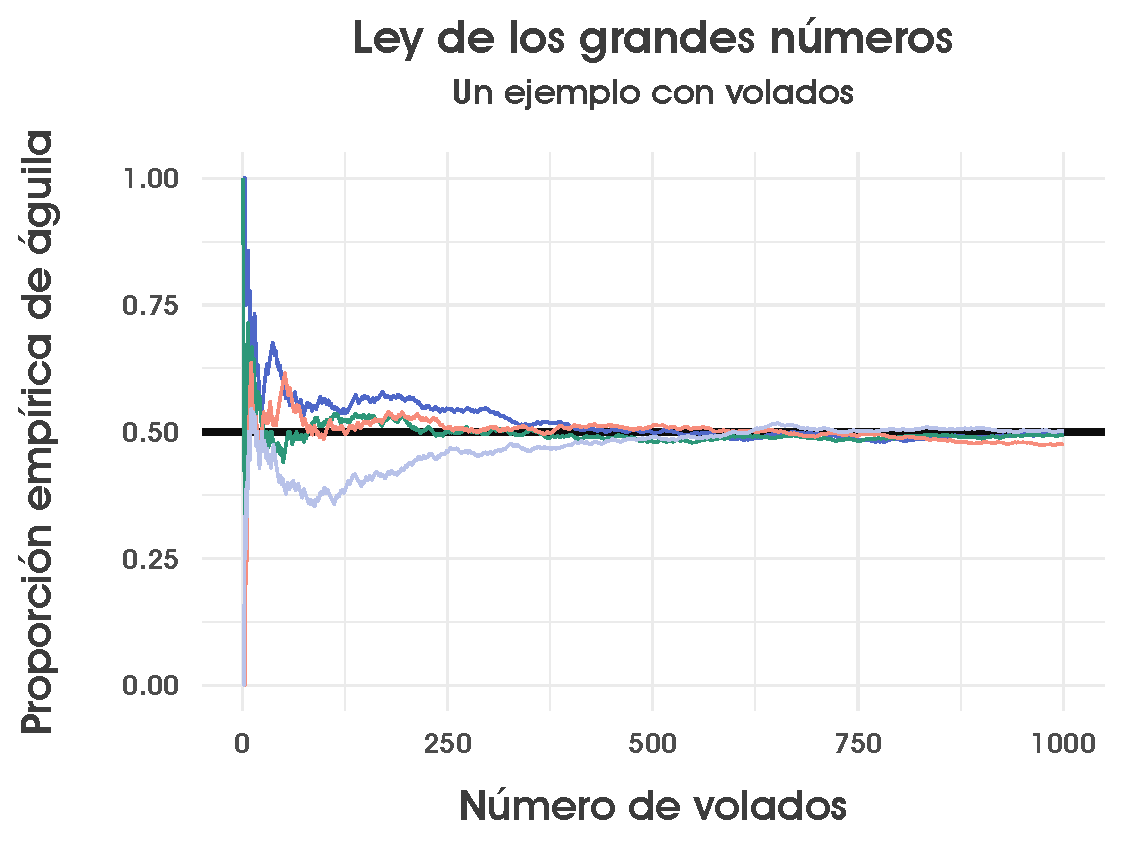
\includegraphics[scale=0.2]{Figs/Bayes/LGN}
	\caption{Ilustración de las leyes de los grandes números mediante volados simulados por computadora. Conforme el número de volados aumenta, la proporción empírica converge a la proporción teórica. Esto pasa para cada serie de volados. Fuente: elaboración propia.}
	\label{fig:LGN}	
\end{figure}

Es cierto que esta práctica de aprender de un sistema, simulando con muestreo aleatorio no surge con las computadoras \parencite{Owen13}. Ya desde 1812 Laplace había sugerido la posibilidad de estimar empíricamente el valor de $\pi$ mediante el llamado problema de la aguja de Buffon \parencite{Ragheb13}. Sin embargo, como el ejemplo de los volados muestra, sí han sido las computadoras las que han potenciado la utilidad de los métodos de simulación. ¿Cuánto hubiéramos tardado en lanzar los 4,000 volados que la computadora simuló al instante? Más aún, esta capacidad computacional consolidó la utilidad de la estadística bayesiana. ¡Y pensar que todo empezó con una guerra y un juego de solitario!, como explico a continuación.

\section{Monte Carlo} 

La simulación por computadora ha permitido el desarrollo de la estadística bayesiana, particularmente desde la década de los 90 del siglo pasado \parencite{RobertCasella11}. Sin embargo, la semilla de este desarrollo ya había sido plantada medio siglo antes desde el terreno de la física, desafortunadamente a causa de la Segunda Guerra Mundial, por los científicos del laboratorio de Los Alamos, encargados del proyecto Manhattan y el desarrollo de más armas de fisión nuclear.\\

Uno de esos científicos fue un matemático polaco-estadounidense llamado Stanislaw Ulam. En 1946, aburrido convaleciendo por una enfermedad, comenzó a preguntarse sobre la probabilidad de ganar en un juego de solitario. Después de mucho batallar con los cálculos de combinatoria se planteó si no sería más práctico estimarla simulando muchas partidas en una de las primeras computadoras electrónicas. Y ahí surgió el eureka: ¿por qué no hacer lo mismo para los problemas de física nuclear en los que estaban trabajando en Los Alamos? \parencite{Eckhardt87}. Al igual que las partidas de solitario, podrían simular muchas realizaciones de los procesos físicos bajo estudio y estimar los resultados más probables.\\ 

Stan compartió su idea con John von Neumann quien, sorprendido y emocionado, le envió una carta a Richard Richtmayer--- el líder del equipo en Los Alamos--- con todos los cálculos necesarios para llevar a cabo el proyecto \parencite{vonNeumann47}. El método fue rápidamente adoptado por todos en Los Alamos, tanto que otro físico, Nicholas Metropolis, sugirió llamarlo \textit{Monte Carlo}, bromeando sobre un tío apostador de Stan, que vivía pidiendo prestado dinero porque ``simplemente tenía que ir a Monte Carlo" \parencite{Metropolis87}. Después de un arduo trabajo, el método pareció funcionar--- gracias en buena medida al trabajo de programación de Klara von Neumann \parencite{Haigh14}--- y el propio Metropolis publicó, junto con Stan, un primer paper presentándolo a grandes rasgos \parencite{MetropolisUlam49}.\\

De manera concreta, el método es la conjunción de la simulación con la ley de los grandes números. Las cantidades que requerían calcular eran valores esperados de la siguiente forma: 
\begin{equation}
\label{eq:IntegralMC}
h^\star = \E{h(Z)}=\int\limits_\mathcal{Z} h(z)f(z)dz ,
\end{equation} 
donde $h$ es una función de interés y $f(z)$ es la distribución de probabilidad sobre las \textit{configuraciones} $z$ en las que podía encontrarse el sistema físico. El gran problema era--- y sigue siendo--- que estas integrales típicamente no pueden calcularse ni analíticamente ni por métodos numéricos tradicionales. Sin embargo, si se tiene una muestra aleatoria de valores de $Z$ provenientes de su distribución $f$, se puede aproximar $h^\star$ con el promedio empírico, que en este contexto se conoce como \textit{estimador de Monte Carlo}: 
\begin{equation*}
h^\star \approx \hat{h} = \sum\limits_{i=1}^N \dfrac{h(z_i)}{N}
\end{equation*}

Entonces, los científicos en Los Alamos se dedicaron a encontrar algoritmos eficientes para obtener una muestra aleatoria de variables provenientes de diferentes distribuciones $f$.\\ 

Lo importante para este trabajo es que este es exactamente el mismo problema que se tiene en la aplicación de la estadística bayesiana y que hizo que por décadas--- por no decir siglos--- fuera poco menos que imposible llevar a cabo análisis bayesianos no triviales, como ya anticipa en \ref{sec:Prob_Analitico}. Muchas de las integrales que surgen en la estadística bayesiana no pueden ser calculadas de manera analítica. El ejemplo más frecuente es la constante normalizadora del teorema de Bayes. ¿Cómo aplicar el teorema si el denominador no puede ser calculado?\\ 

No obstante, la forma de \eqref{eq:IntegralMC} permite llevar a cabo una gran variedad de \textit{resúmenes inferenciales} \parencite{GP97}. La posibilidad de realizar las correspondientes \textit{integraciones por Monte Carlo} hace que, en la práctica, exista una dualidad entre una distribución o densidad y una muestra proveniente de ella \parencite{SmithGelfand92}. La única receta de la inferencia bayesiana--- ver la página \pageref{receta_bayesiana}---, en la práctica se convierte en obtener una muestra aleatoria de la distribución posterior lo suficientemente grande para, con ella, estimar por Monte Carlo los resúmenes inferenciales requeridos.\\

Hay varios métodos de simulación de variables aleatorias que permiten obtener muestras aleatorias independientes y calcular un estimador de Monte Carlo. Entre los más mencionados podemos encontrar el método de inversión, el de aceptación y rechazo o el muestreo por importancia \parencites{Ross13,RobertCasella10}. Sin embargo, los físicos de Los Alamos pronto se dieron cuenta que, en lugar de buscar realizar directamente simulaciones independientes, era más práctico hacer simulaciones secuenciales que dependieran entre sí. 

\section{MCMC}

La forma de realizar simulaciones correlacionadas que logren simular de manera más eficiente que los métodos directos tradicionales de aceptación y rechazo o muestreo por importancia es utilizar \textit{cadenas de Markov}.

\dfn{\textbf{Cadena de Markov}\\
\label{def:Cadena_Markov}
Una \textit{cadena de Markov} $\left\lbrace Z^{(n)}, \, n = 0, 1, 2,\dots \right\rbrace$ es una secuencia de variables aleatorias tales que satisfacen la siguiente \textit{propiedad de Markov} para toda $n$
\begin{equation*}
Z^{(n+1)}| Z^{(n)}, \dots, Z^{(0)} \sim Z^{(n+1)}| Z^{(n)} \sim p(z^{(n+1)}|z^{(n)})
\end{equation*}
}
Si llamamos \textit{estados} a los eventos que suceden en la cadena en cada punto en el tiempo, podemos decir que la distribución condicional del estado futuro de una cadena de Markov dada toda su historia depende exclusivamente del estado presente y no de los estados anteriores. Dicho de otra forma, \textit{el futuro es independiente del pasado, dado el presente}. La distribución condicional se llama \textit{kernel de transición}, mismo que normalmente es también independiente del índice $n$ y depende exclusivamente del estado actual y el estado futuro. Esta propiedad se llama \textit{homogeneidad} en el tiempo y permite simplificar la notación a $p(\tilde{z}|z)$.\\ 

La teoría de cadenas de Markov determina las condiciones bajo las cuales existen teoremas límites al estilo de las leyes de los grandes números y que en este contexto se conocen como \textit{ergódicos}. Esta teoría escapa los objetivos particulares de la tesis pero, si es de interés para el lector, algunas referencias útiles son \textcites{Rincon12,Neal93,Ross96,TaylorKarlin84}. Baste decir por ahora que, bajo ciertas condiciones, sabemos que la distribución de $Z^{(n)}$ converge a una distribución límite conforme $n$ tiende a infinito. Más aún, los \textit{promedios ergódicos}--- es decir los promedios acumulados de la cadena--- también convergen al valor esperado de la distribución límite. Esto se puede expresar matemáticamente como sigue:
\begin{subequations}\label{eq:Teo_Erg}
\begin{align}
Z^{(N)} &\xrightarrow[N\rightarrow\infty]{\mathcal{D}} Z, \quad Z \sim f(z) \label{eq:Teo_Erg_Conv_D} \\
\dfrac{1}{N}\sum\limits_{n=1}^N h\left(z^{(n)}\right) &\xrightarrow[N\rightarrow\infty]{} \mathbb{E}_{f}[h(z)]
\label{eq:Teo_Erg_Conv_Prom}
\end{align}
\end{subequations}

Esto da lugar a los métodos de \textit{Markov Chain Monte Carlo} o MCMC en los que el objetivo es construir una cadena de Markov que satisfaga las condiciones necesarias y cuya distribución límite sea la distribución de la cual se quiere simular. Así, después de $N$ transiciones de la cadena, la simulación convergería a la distribución objetivo y se podría estimar la cantidad de interés $h^\star$ mediante el estimador de MCMC: 

\begin{equation*}
h^\star \approx \hat{h} = \sum\limits_{n=1}^N \dfrac{h\left(z^{(n)}\right)}{N}
\end{equation*}

\subsection{Metropolis Hastings}

 El primero de estos métodos MCMC fue propuesto por las parejas de esposos Arianna y Marshall Rosenbluth y Augusta y Edward Teller junto con el propio Nicholas Metropolis en el \textit{Journal of Chemical Physics} \parencite{Metropolis53}. Se conoce como el algoritmo de Metropolis, aunque hay quienes creen que en realidad el trabajo más fuerte lo hicieron el resto de los autores por lo que debería llamarse el algoritmo de Rosenbluth-Teller \parencite{Gubernatis05}. Casi 20 años después, el estadístico canadiense Wilfred Keith Hastings lo generalizó \parencite{Hastings70}, por lo que podemos hablar de algoritmos de Metropolis Hastings o MH.

\subsubsection*{Balance detallado, la clave de MH}
 
Las cadenas de Markov para MH requieren ser homogéneas en el tiempo y que sea posible llegar a cualquier estado en un número finito de transiciones, algo que se conoce como \textit{irreducibilidad}. Si además el kernel de transición satisface la siguiente \textit{ecuación de balance detallado} para alguna distribución $f$, se dice que es \textit{reversible} y podemos aplicar el teorema ergódico.
\begin{equation}
\label{eq:Balance_Detallado}
f(z)p(\tilde{z}|z)=f(\tilde{z})p(z|\tilde{z})
\end{equation}

El algoritmo de Metropolis Hastings busca construir cadenas de Markov homogéneas, irreducibles y reversibles que tengan como distribución límite a la distribución objetivo. ¿Cómo hacerlo? Para ello analicemos lo que la reversibilidad implica de manera intuitiva.\\

Siguiendo la argumentación de \textcite{ChibGreenberg95}, \eqref{eq:Balance_Detallado} refleja que hay un balance entre las probabilidades de la cadena de estar en diferentes estados, de ahí el nombre. Supongamos que no se cumpliera la reversibilidad para algún kernel $q(\tilde{z}|z)$. Entonces, sin pérdida de generalidad, para algunos estados pasaría que:
\begin{equation}
\label{eq:Inbalance_Detallado}
\dfrac{f(z)}{f(\tilde{z})}>\dfrac{q(z|\tilde{z})}{q(\tilde{z}|z)}
\end{equation}

De manera un poco informal, tenemos que el miembro izquierdo de la desigualdad refleja las probabilidades relativas ``necesarias'' entre estar en el estado $z$ y el estado $\tilde{z}$. El miembro derecho, por su parte, indica las probabilidades relativas de transitar a dichos estados bajo el kernel de transición de la cadena. La desigualdad indica que la cadena estaría transitando a $\tilde{z}$ más de lo necesario y, equivalentemente, transitaría a $z$ menos de lo necesario.\\ 

Para conseguir el balance requerido para aplicar el teorema ergódico, necesitamos hacer una \textit{corrección de Metropolis} al kernel de transición, reduciendo el número relativo de veces que la cadena transite de $z$ a $\tilde{z}$ y aumentando el número relativo de transiciones de $\tilde{z}$ a $z$. La forma de hacer la corrección es comenzar con un kernel, $q(\tilde{z}|z)$, que \textit{proponga} un estado y agregar una \textit{probabilidad de aceptación} $\alpha(\tilde{z};z)$. Si la propuesta es rechazada, la cadena permanece en el mismo estado, reduciendo a la vez el número de transiciones hacia estados sobremuestreados y aumentando el número relativo de veces que estamos en el estado originalmente submuestreado. Estos dos pasos constituyen un kernel de transición de Metropolis Hastings de la siguiente forma: 
\begin{align*}
p_{\scriptscriptstyle{MH}}(\tilde{z}|z) &= q(\tilde{z}|z)\alpha(\tilde{z};z) \quad z \neq \tilde{z} \\
p_{\scriptscriptstyle{MH}}(z|z) &= 1 - \int\limits_{\tilde{\mathcal{Z}}} p_{\scriptscriptstyle{MH}}(\tilde{z}|z)d\tilde{z}
\end{align*}

Queremos que el kernel $p_{\scriptscriptstyle{MH}}$ satisfaga \eqref{eq:Balance_Detallado}, esto es:
\begin{equation*}
f(z)p_{\scriptscriptstyle{MH}}(\tilde{z}|z)=f(\tilde{z})p_{\scriptscriptstyle{MH}}(z|\tilde{z}) \quad \Leftrightarrow \quad f(z)q(\tilde{z}|z)\alpha(\tilde{z};z)=f(\tilde{z})q(z|\tilde{z})\alpha(z;\tilde{z}) 
\end{equation*}

De acuerdo a nuestra desigualdad supuesta en \eqref{eq:Inbalance_Detallado}, las transiciones de $\tilde{z}$ a $z$ se dan demasiado poco, por lo que siempre deberíamos aceptar este tipo de transiciones a fin de corregir el submuestreo. Tomemos entonces $\alpha(z;\tilde{z}) = 1$ y observemos que $\alpha(\tilde{z};z)$ queda determinada de tal forma que logremos el balance necesario: 
\begin{equation*}
\alpha(\tilde{z};z)=\dfrac{f(\tilde{z})q(z|\tilde{z})}{f(z)q(\tilde{z}|z)}
\end{equation*}

Si la desigualdad \eqref{eq:Inbalance_Detallado} fuera en el sentido contrario, i.e. $f(\tilde{z})q(z|\tilde{z})>f(z)q(\tilde{z}|z)$, los roles de las probabilidades de aceptación se invertirían, por lo que de manera general tenemos que 
\begin{equation}
\label{eq:Proba_Aceptar_MH}
\alpha(\tilde{z};z)=min\left\lbrace\dfrac{f(\tilde{z})q(z|\tilde{z})}{f(z)q(\tilde{z}|z)},1\right\rbrace
\end{equation}

La utilidad de MH para la estadística bayesiana está en la forma de la probabilidad de aceptación en \eqref{eq:Proba_Aceptar_MH}. Como la distribución objetivo se encuentra tanto en el denominador como en el numerador, no se requiere completa sino basta con conocerla salvo por una constante de proporcionalidad que desaparezca al realizar el cociente. Esta situación es exactamente la que impera en la aplicación de la estadística bayesiana. Recordemos el resumen del aprendizaje bayesiano en \eqref{eq:Bayes_Prop}, \textit{la posterior es proporcional a la inicial por la verosimilitud}: 
\begin{equation*}
f(\theta|y) \propto L(\theta)f(\theta).
\end{equation*}

Por esto, para simular valores de una distribución posterior $f(\theta|y)$ mediante MH solo necesitamos la distribución inicial $f(\theta)$, la verosimilitud $L(\theta)=f(y|\theta)$ y un kernel de propuestas $q(\tilde{\theta}|\theta)$, siguiendo el \textbf{Algoritmo \ref{alg:MH}}. Hay una última consideración que debe tenerse en cuenta y es que la posterior sea propia; si se inició con una inicial impropia es posible que la posterior no pueda integrar a 1, lo que haría que el algoritmo fallara \parencite{RobertCasella10}.\\

\begin{algorithm}
\DontPrintSemicolon
Valor inicial arbitrario o simulado $\theta^{(0)}$\;
\For{$n \leftarrow 1$ \KwTo $N$}{
$\theta \leftarrow \theta^{(n-1)}$\;
$\tilde{\theta} \sim q(\tilde{\theta}|\theta)$\;
$\alpha(\tilde{\theta};\theta) \leftarrow min\left\lbrace\dfrac{f(y|\tilde{\theta})f(\tilde{\theta})q(\theta|\tilde{\theta})}{f(y|\theta)f(\theta)q(\tilde{\theta}|\theta)},1\right\rbrace$\;
$u \sim U[0,1]$ \;
\eIf{$u \leq \alpha(\tilde{\theta};\theta)$}{
	$\theta^{(n)} \leftarrow \tilde{\theta}$\;
	}{
	$\theta^{(n)} \leftarrow \theta $\;
	}
}

\caption{Metropolis Hastings para el aprendizaje bayesiano \label{alg:MH}}
\end{algorithm}

\subsubsection*{\textit{Random Walk Metropolis}}

Si la posterior es propia, entonces el mayor problema, claro está, es el de encontrar un kernel de propuestas conveniente. Una alternativa son aquellos que exploran progresivamente el espacio de estados de manera local. Estos se conocen como \textit{Random Walk Metropolis} o RWM \parencite{RobertCasella10}. De hecho, el algoritmo inicial de \textcite{Metropolis53} era de este tipo, usando una distribución uniforme en una vecindad del estado actual; pero también se pueden usar otras distribuciones, como una normal o una $t$ de Student centrada en dicho estado. \textcite{Robert15} hace la analogía con alguien que para ver una pintura en un cuarto oscuro tiene que ir alumbrando el cuadro con una antorcha, iluminando secuencialmente diferentes segmentos del lienzo.\\

Estos kérneles de caminata aleatoria resultan ser \textit{simétricos}--- esto es,  $q(\tilde{\theta}|\theta) = q(\theta |\tilde{\theta})$--- lo que simplifica los cálculos de probabilidades de aceptación:
\begin{equation*}
\alpha_{RWM}(\tilde{\theta};\theta)=min\left\lbrace\dfrac{f(\tilde{\theta}|y)q(\theta|\tilde{\theta})}{f(\theta|y)q(\tilde{\theta}|\theta)},1\right\rbrace = min\left\lbrace\dfrac{f(\tilde{\theta}|y)}{f(\theta|y)},1\right\rbrace
\end{equation*}

Un ejemplo trivial puede ayudar a visualizar cómo funcionan. Supongamos que quisiéramos simular de una posterior que, en realidad, es una normal bivariada cuyas marginales son normales estándar. Un posible kernel de transición sería una distribución uniforme en un rectángulo de $3$ de lado centrado en el estado actual de la cadena, por lo que tendríamos un kernel simétrico y un algoritmo de \textit{Random Walk Metropolis}.\\ 

Podemos ver cómo se va explorando el espacio de estados en la \textbf{Figura \ref{fig:RWM}}. Cuando una de las propuestas es rechazada, esta se marca como una tache. Empezando en un punto alejado del origen, la cadena comienza a acercarse a la región de mayor densidad. En el fondo--- como espero explicar más claro después--- encontrar esta \textit{región crítica} y explorarla lo suficientemente bien para poder calcular los resúmenes inferenciales de interés es el verdadero objetivo de un algoritmo de integración por MCMC \parencites{Neal93,Betancourt17}. Con tan solo 2,500 iteraciones la cadena ya la recorrió varias veces y los valores que alejarían a la cadena de la misma son normalmente rechazados. Podemos ver también cómo los promedios ergódicos van acercándose a $0$ para ambas variables.\\

Pero la pregunta permanece, ¿cómo determinar el kernel de propuestas? ¿Por qué usar $3$ como lado y no $0.5$? ¿Qué hubiera pasado en ese caso? Podemos observarlo en la \textbf{Figura \ref{fig:RWM2}}. El rectángulo de propuestas es más pequeño y eso tiene dos efectos: hay menos propuestas rechazadas pero la cadena avanza más lentamente. Vemos cómo aún después de las mismas 2,500 iteraciones la cadena no ha explorado por completo el área de mayor densidad y los promedios ergódicos apenas comienzan a converger.\\ 

\begin{figure}[h]
    \centering
    \begin{subfigure}{0.3\textwidth}
        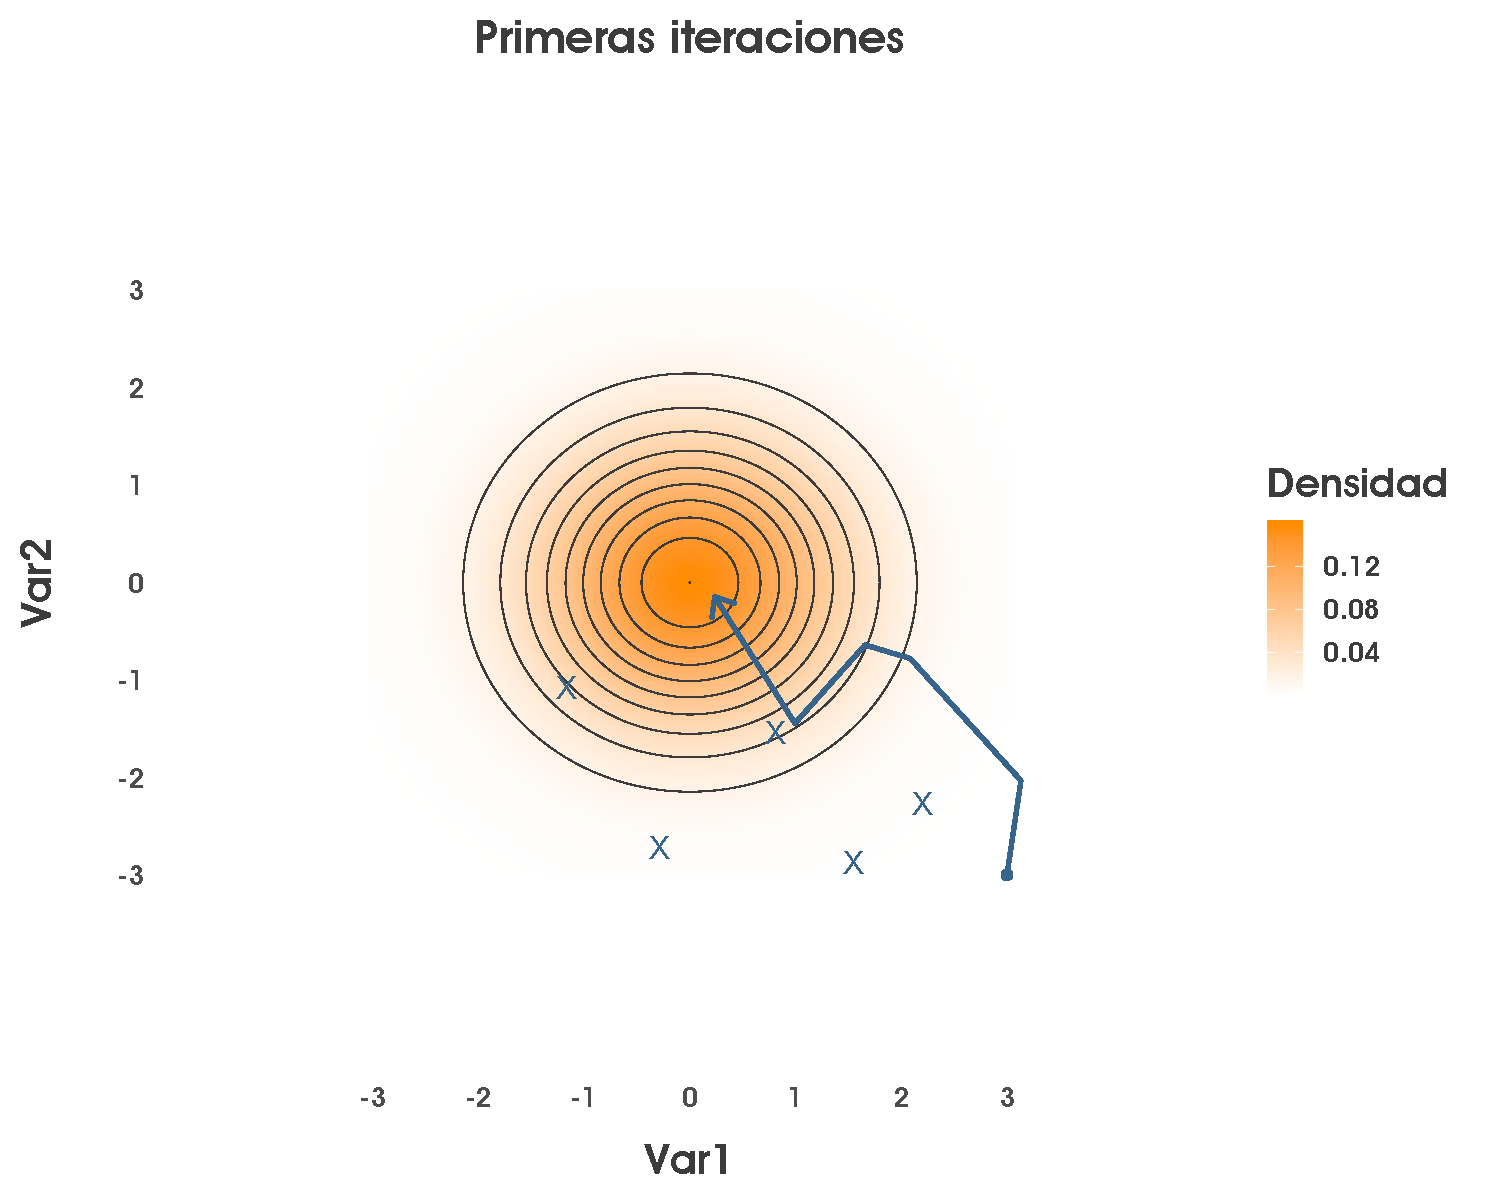
\includegraphics[width=\textwidth]{Figs/Bayes/Ejemplo_RWM_A}
        \caption{La cadena empieza lejos de las zonas de mayor densidad y se va acercando a ellas. Las taches representan propuestas rechazadas.}
    \end{subfigure}
    ~ 
    \begin{subfigure}{0.3\textwidth}
        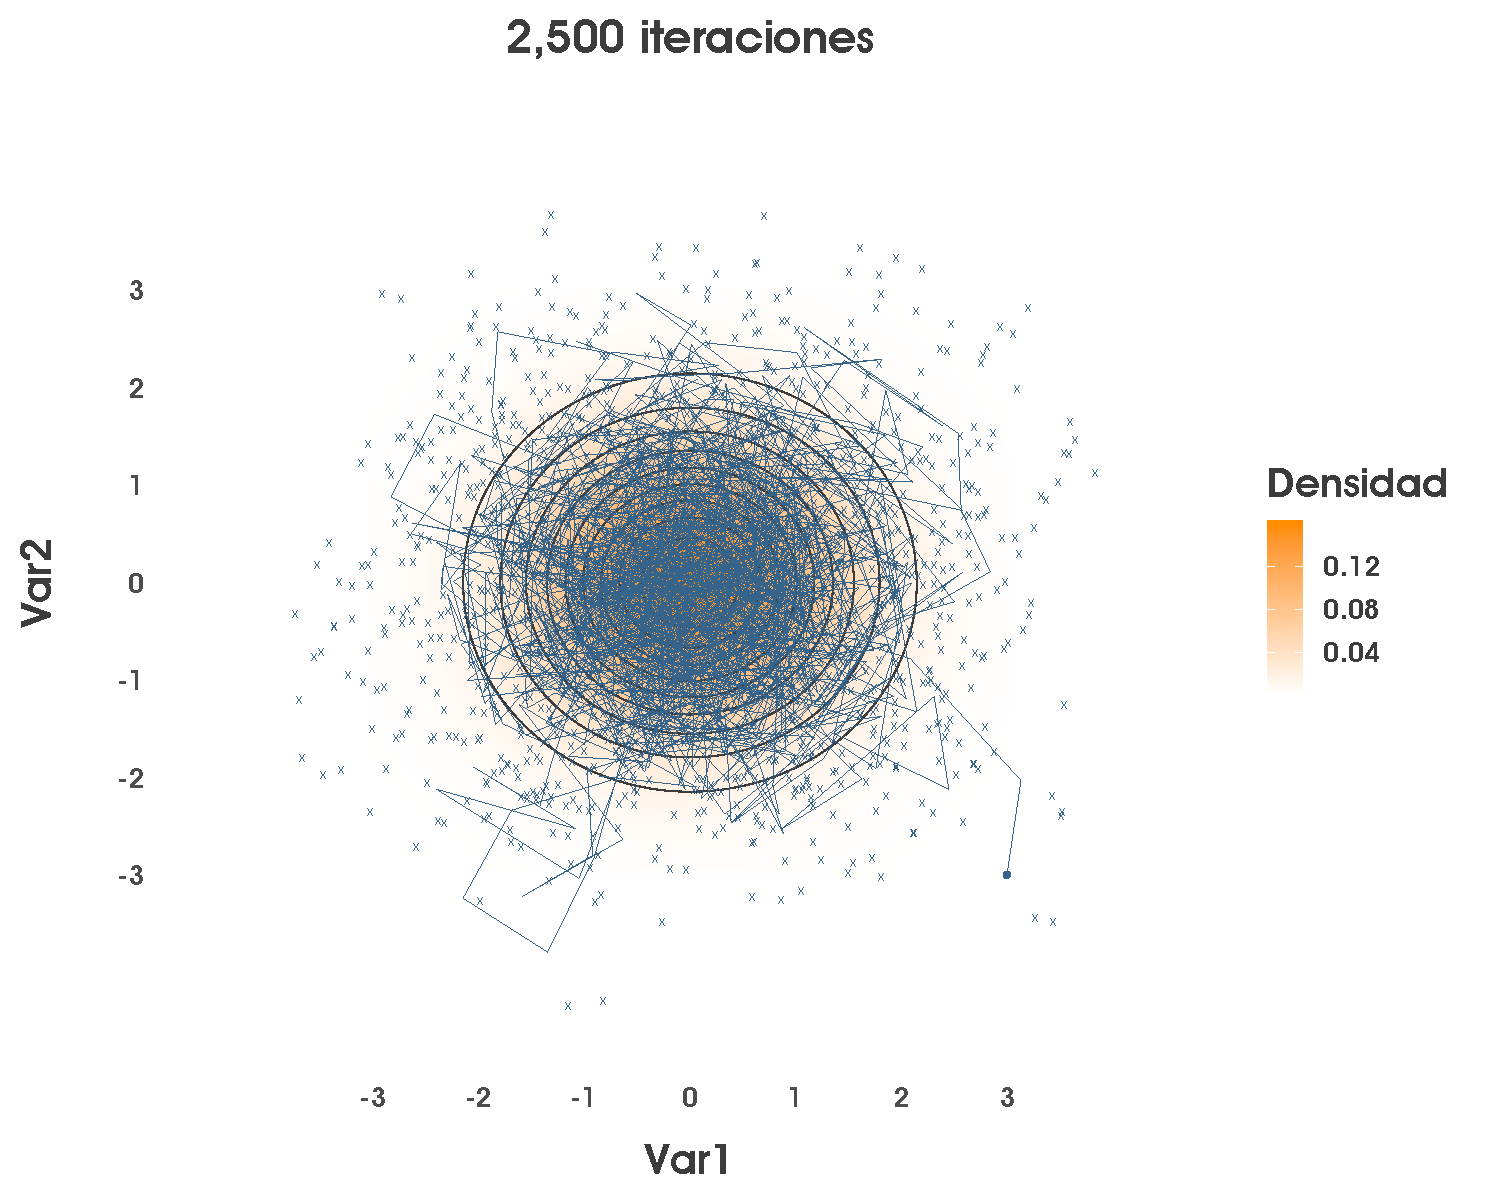
\includegraphics[width=\textwidth]{Figs/Bayes/Ejemplo_RWM_B}
        \caption{Después de 2,500 iteraciones, la cadena explora ya la región crítica. Los valores fuera de ella normalmente son rechazados.}
    \end{subfigure}
    ~
    \begin{subfigure}{0.3\textwidth}
        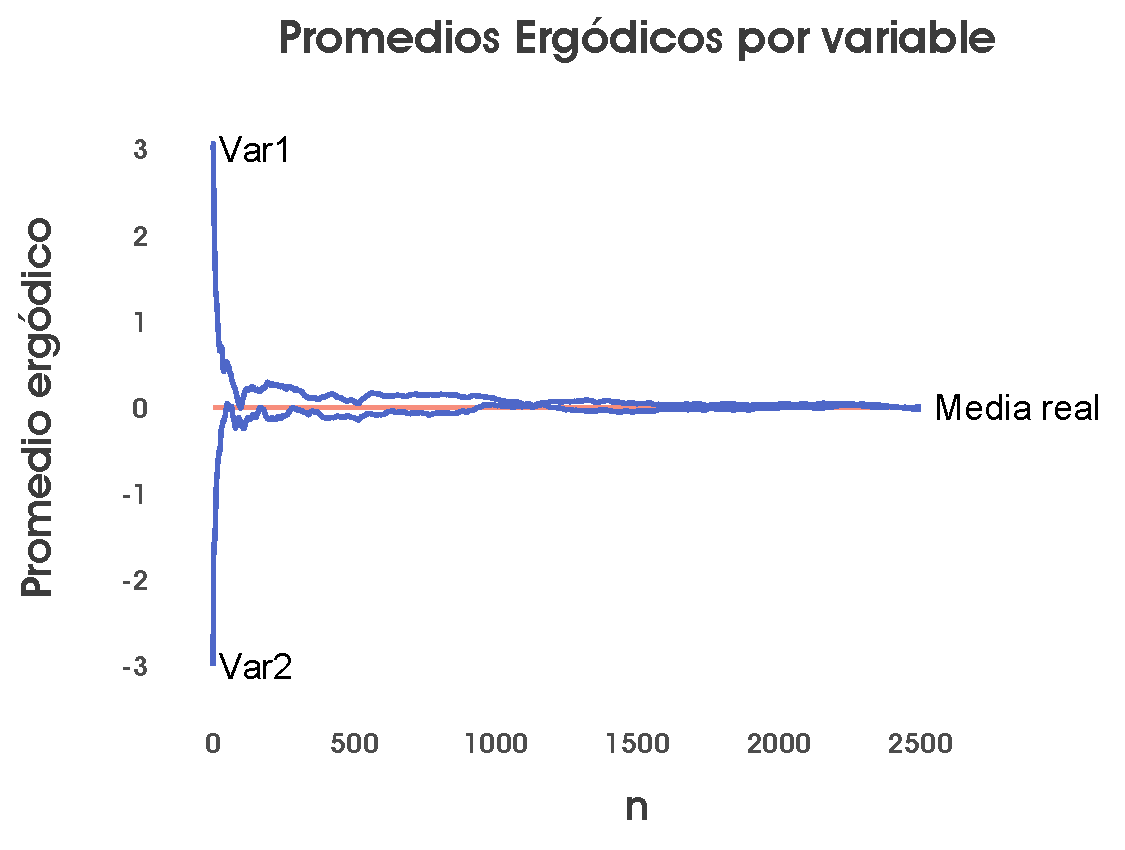
\includegraphics[width=\textwidth]{Figs/Bayes/Ejemplo_RWM_C}
        \caption{Los promedios ergódicos van convergiendo a las medias teóricas.}
    \end{subfigure}
    \caption{Ilustración de una cadena de Metropolis Hastings simulando de una normal bivariada sin correlación mediante una implementación de \textit{Random Walk Metropolis}. Fuente: elaboración propia.}\label{fig:RWM}
\end{figure}

\begin{figure}[h]
    \centering
    \begin{subfigure}{0.3\textwidth}
        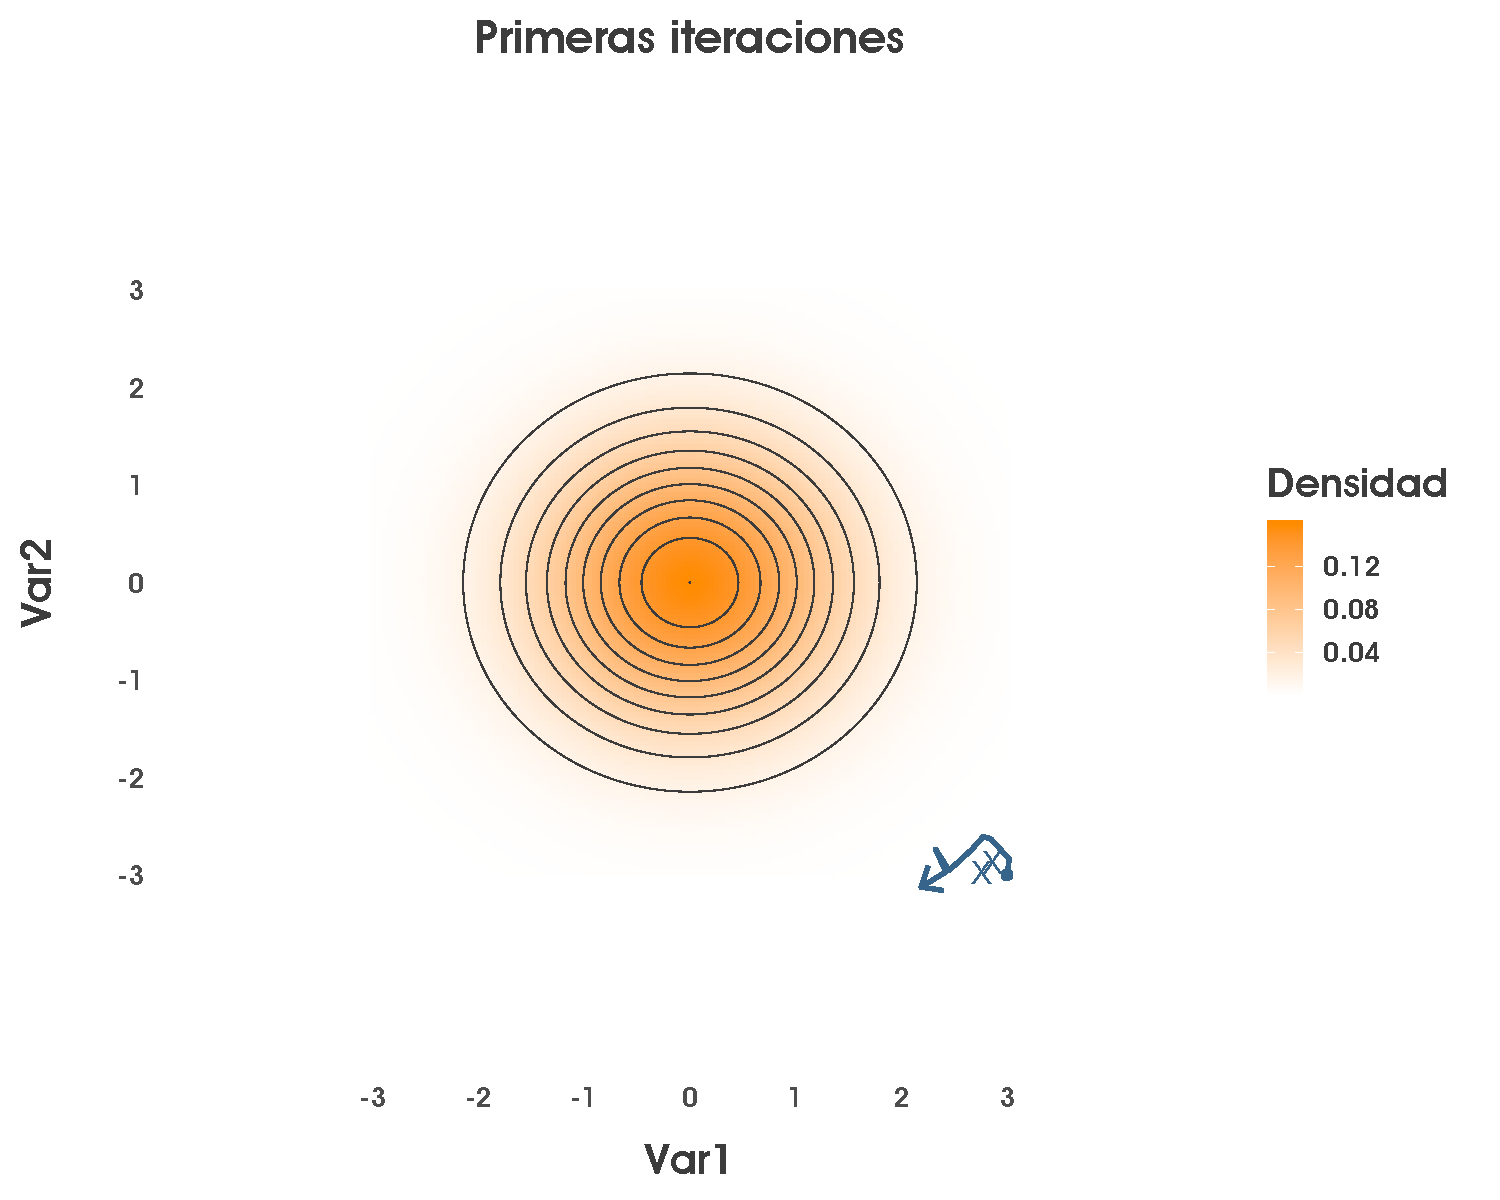
\includegraphics[width=\textwidth]{Figs/Bayes/Ejemplo2_RWM_A}
        \caption{La cadena empieza lejos de las zonas de mayor densidad y avanza lentamente. Las taches representan propuestas rechazadas.}
    \end{subfigure}
    ~ 
    \begin{subfigure}{0.3\textwidth}
        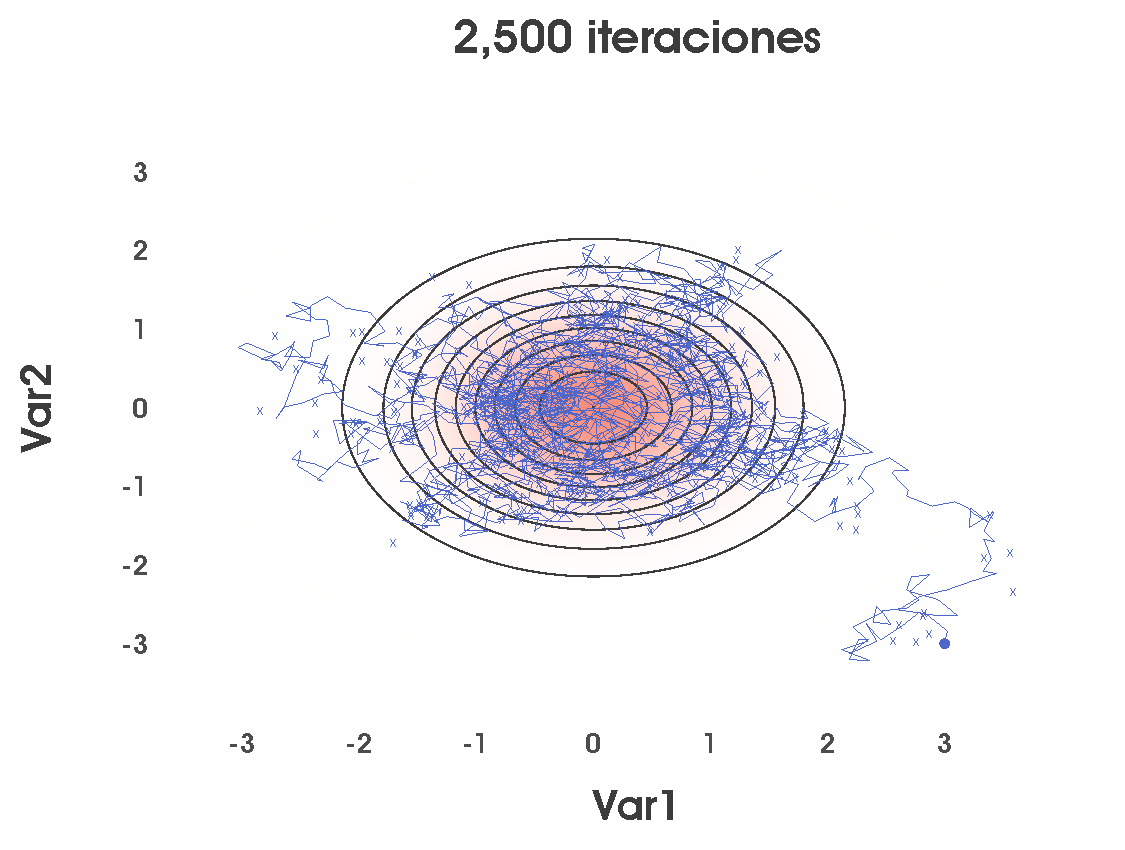
\includegraphics[width=\textwidth]{Figs/Bayes/Ejemplo2_RWM_B}
        \caption{Después de 2,500 iteraciones, la cadena no ha explorado la región crítica, aunque hay menos propuestas rechazadas.}
    \end{subfigure}
    ~
    \begin{subfigure}{0.3\textwidth}
        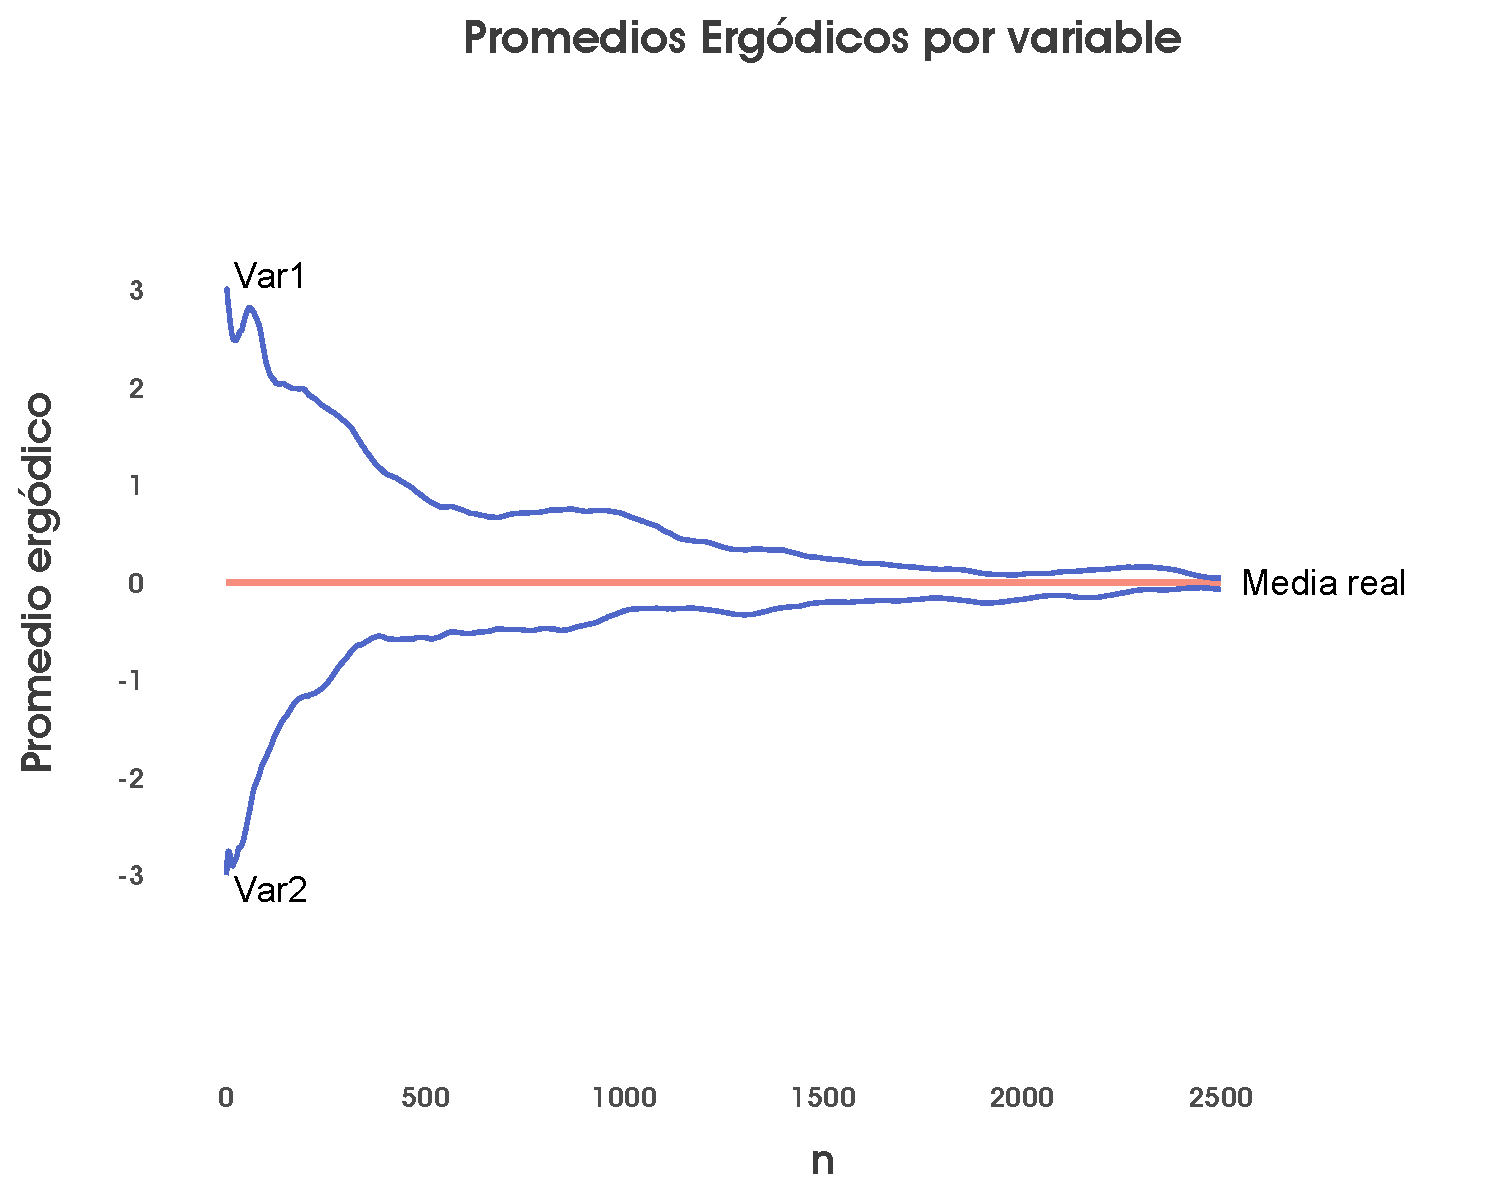
\includegraphics[width=\textwidth]{Figs/Bayes/Ejemplo2_RWM_C}
        \caption{Los promedios ergódicos tardan en converger.}
    \end{subfigure}
    \caption{Ilustración de una cadena de Metropolis Hastings simulando de una normal bivariada sin correlación mediante una implementación de \textit{Random Walk Metropolis} con un kernel de propuestas estrecho. Fuente: elaboración propia.}\label{fig:RWM2}
\end{figure}

El rectángulo más amplio propone valores que se alejan de la región crítica, mismos que tienden a ser rechazados. Sin embargo, también permite proponer valores más distantes del punto actual, lo que en este caso hace que la cadena avance rápidamente. El rectángulo más pequeño avanza más bien ``lento pero seguro''... quizás demasiado lento. Ambas cadenas convergerán, pero este ejemplo ilustra uno de los principales problemas de los algoritmos de MH, en general.\\ 

Elegir un kernel de propuestas eficiente no es sencillo. Si la escala del kernel es demasiado pequeña, los saltos son demasiado pequeños y la cadena avanza demasiado lento. Si la escala es demasiado grande, corremos el riesgo de que la cadena rechace casi todas las propuestas y quede ``atorada'' en algún lugar; si la cadena repite el mismo valor varias veces seguidas, también alenta su avance. Debe haber un justo medio entre ambos extremos. Esto podemos verlo comparando el comportamiento de tres kérneles cuando intentan simular normales ahora altamente correlacionadas, en la \textbf{Figura \ref{fig:RWM_Corr}}.\\ 

\begin{figure}[h]
    \centering
    \begin{subfigure}{0.3\textwidth}
        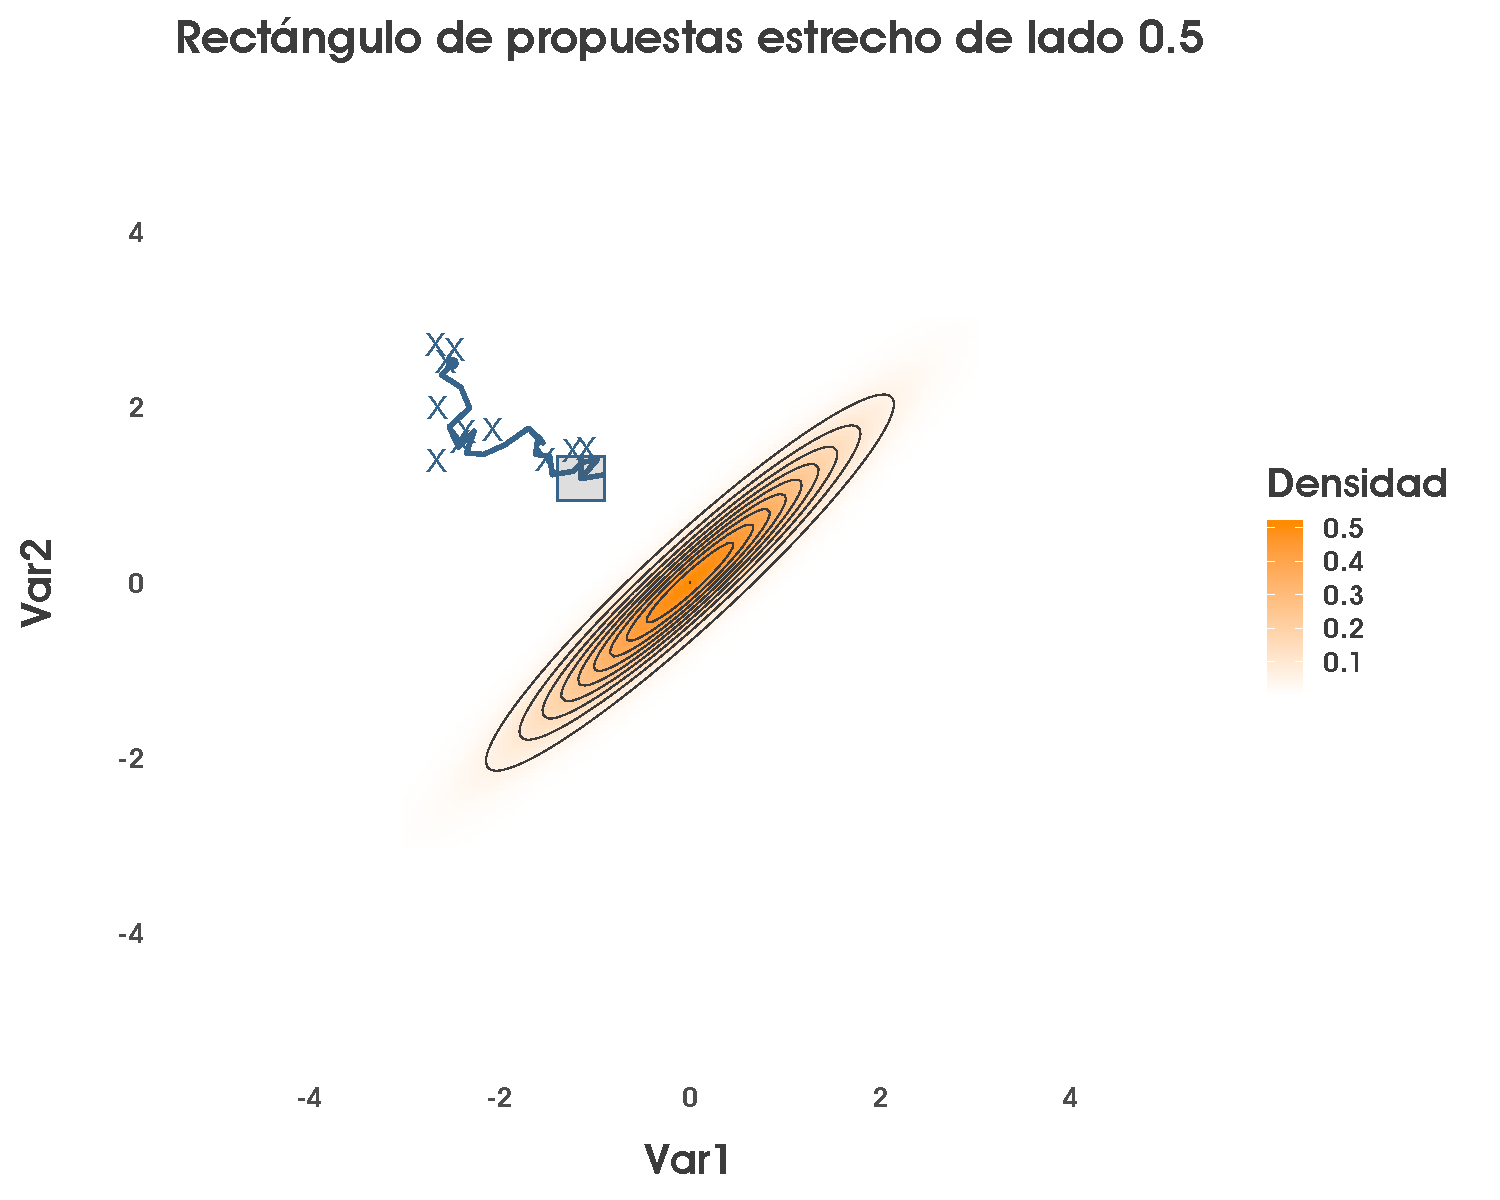
\includegraphics[width=\textwidth]{Figs/Bayes/Ejemplo_RWM_Compara1}
        \caption{Un kernel de propuestas demasiado estrecho acepta más propuestas pero se mueve lento.}
    \end{subfigure}
    ~ 
    \begin{subfigure}{0.3\textwidth}
        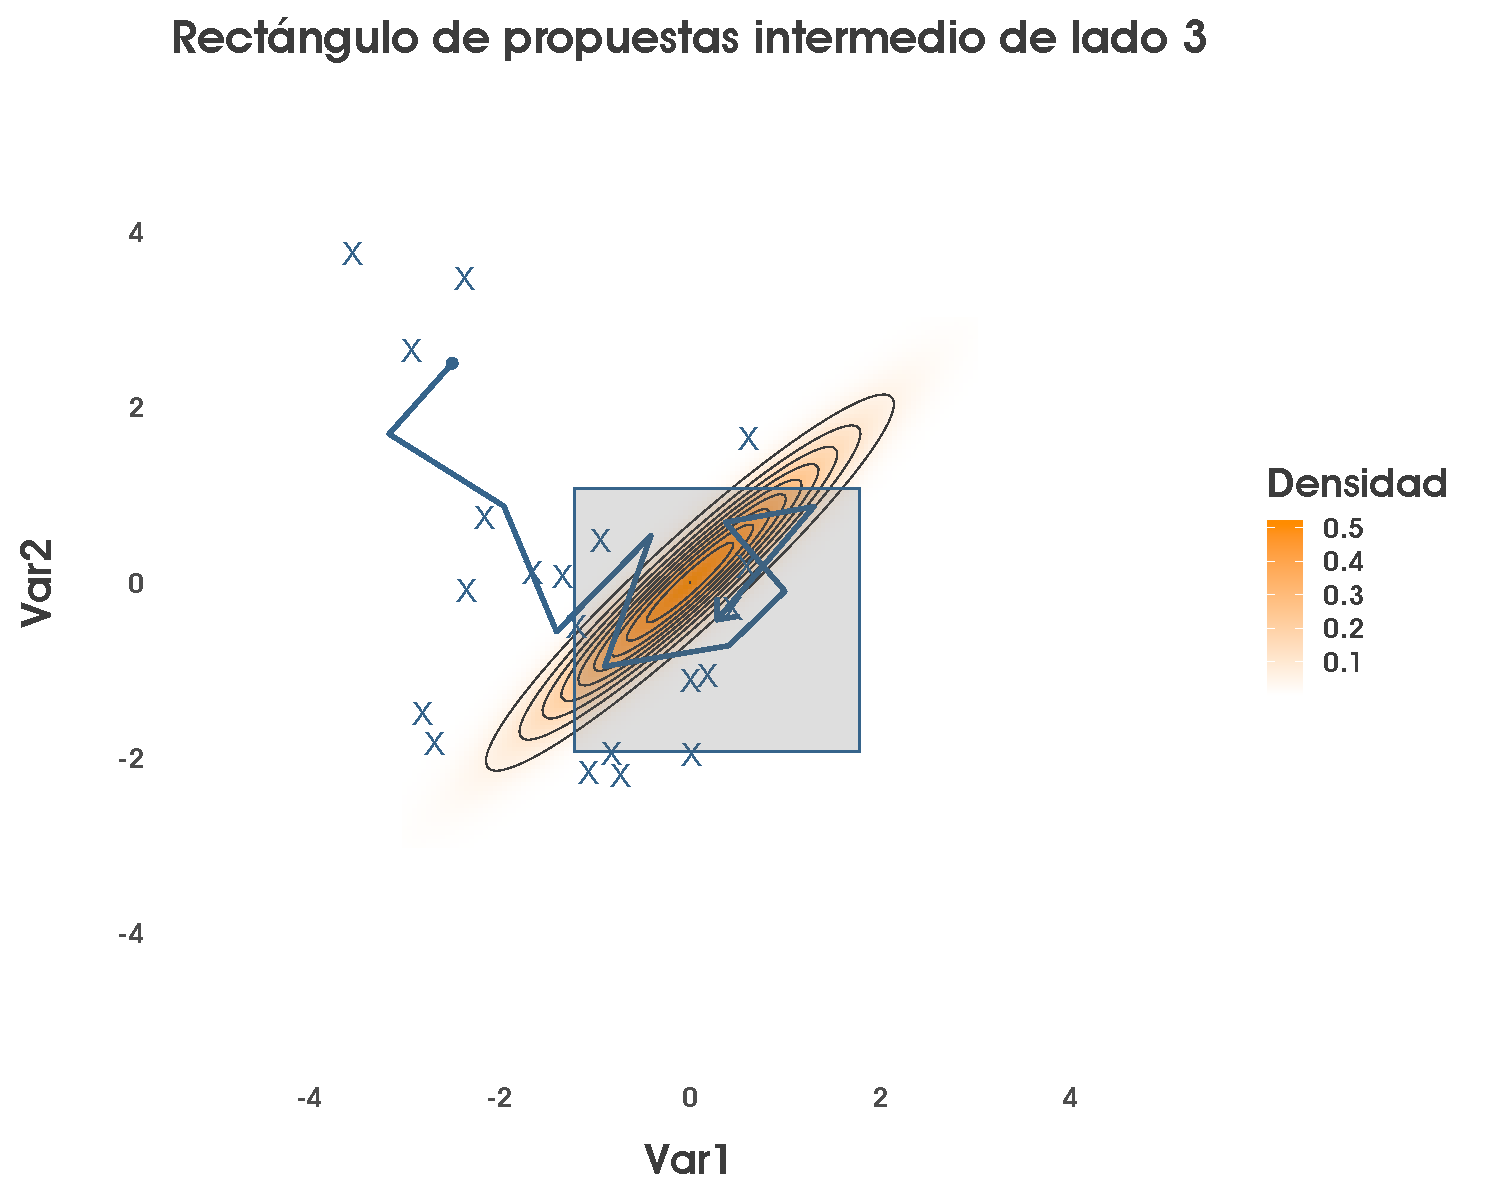
\includegraphics[width=\textwidth]{Figs/Bayes/Ejemplo_RWM_Compara2}
        \caption{El kernel óptimo en general es uno que permita alcanzar regiones diferentes del espacio sin rechazar ``demasiadas'' propuestas. Esto permite que la cadena avance de mejor manera.}
    \end{subfigure}
    ~
    \begin{subfigure}{0.3\textwidth}
        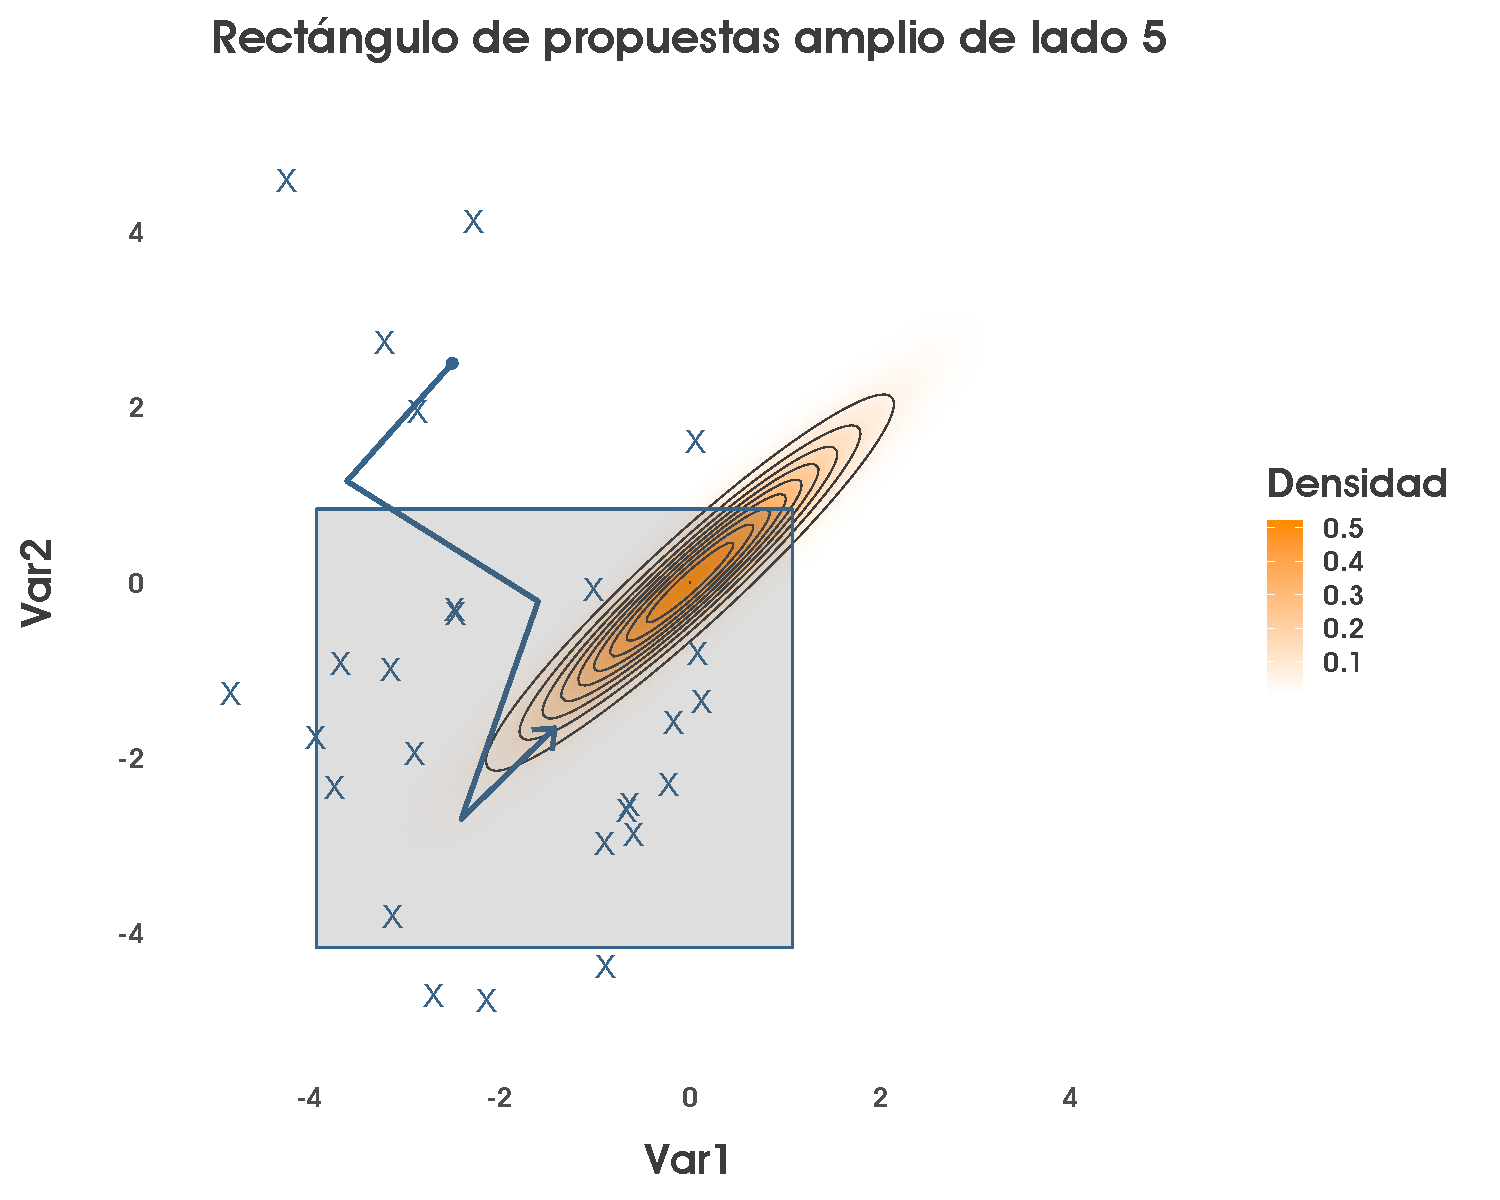
\includegraphics[width=\textwidth]{Figs/Bayes/Ejemplo_RWM_Compara3}
        \caption{Un kernel de propuestas demasiado amplio rechaza demasiadas propuestas. Esto puede provocar que la cadena quede ``atorada'' en el mismo lugar por varias propuestas, lo que a su vez implica un avance más lento.}
    \end{subfigure}
    ~
    \caption{Comparación de kerneles uniformes de propuestas para simular una normal bivariada con correlación $0.95$ mediante RWM. Las tres cadenas presentan las primeras $30$ transiciones, aunque no se distingan las repeticiones de los puntos en los que la cadena permanece en el mismo estado. Fuente: elaboración propia.}\label{fig:RWM_Corr}
\end{figure}

Ciertamente hay investigación enfocada a proponer ``reglas de dedo'' que sean relativamente eficientes \parencites{GelmanRobertsGilks96,Geyer05,YangRdz13}. Para el ejemplo original de normales bivariadas no correlacionadas elegí el rectángulo uniforme de lado $3$ porque \textcite{YangRdz13} encuentran que este es el ancho óptimo para simular una normal estándar mediante un kernel uniforme. El uso del kernel uniforme se debe a que es fácil de entender y fue el utilizado por los científicos de Los Álamos, pero pueden haber kérneles más eficientes como reporta el mismo artículo.\\ 

 El problema crece porque la dimensionalidad de los problemas hace que muy rápidamente nos alejemos de los ejemplos triviales y sea mucho más difícil proponer kérneles de transición que funcionen de manera adecuada. ¿Qué hacer? Por varios años esto desalentó el uso de los métodos MCMC, hasta la década de los 90 cuando hubo una ``epifanía'' en el mundo de la estadística bayesiana \parencite{RobertCasella11}. 

\subsection{Gibbs Sampler}

Alan Gelfand y Adrian Smith presentaron en 1990 un artículo titulado \textit{Sampling-Based Approaches to Calculating Marginal Densities} \parencite{GelfandSmith90}. En él rescataron tres algoritmos de simulación para obtener densidades que no pueden ser conocidas de manera analítica. Sin embargo, el que provocó la explosión de los métodos bayesianos fue el llamado \textit{Gibbs Sampler}. Este algoritmo de MCMC fue propuesto por los hermanos Stuart y Donald Geman mientras trabajaban en problemas de reconstrucción de imágenes \parencite{GemanGeman84}, pero ya estaba oculto en el artículo de \textcite{Hastings70} cuando sugería que para simular de una distribución multidimensional se podría cambiar de manera secuencial una única coordenada o, incluso, subgrupos de coordenadas.\\ 

En otras palabras, ``divide y vencerás''; si el problema es que la distribución objetivo es de alta dimensionalidad y compleja, ¿por qué no intentar simularla por partes más simples en lugar de querer simularla directamente? La gran contribución de los hermanos Geman fue encontrar una manera simple y poderosa de llevarlo a cabo. La chispa de Gelfand y Smith fue mostrarle al mundo estadístico que--- sin ser el método óptimo para cualquier problema--- podía ser bastante eficiente en un amplio rango de problemas comúnmente encontrados en la práctica y, mejor aún, era efectivamente simple y universal \parencite{GelfandEtAl90}.\\

Supongamos que el vector que queremos simular es bivariado, digamos $Z = (X,Y)$. El algoritmo consiste en alternar simulaciones simples de cada variable condicional en la otra, conservando los vectores bivariados de cada ciclo de dos \textit{pasos de Gibbs}. Primero simulamos de $X|Y$, luego de $Y|X$; volvemos a simular otra $X$ dada la $Y$ anterior, luego otra $Y$ dada la nueva $X$ y así sucesivamente. Una analogía imperfecta pero que me funciona como recurso pnemotécnico para recordar el \textit{Gibbs Sampler} es imaginar que mi objetivo es cruzar de algún punto en una acera a otro en la acera contraria. En lugar de cruzar la calle de manera diagonal en un solo paso, cruzamos mediante dos. El primero es caminar por la misma banqueta hasta alguna esquina o lugar indicado y el segundo es cruzar la calle sobre el paso peatonal. Estos dos pasos constituirían una \textit{transición de Gibss} y repitiendo transiciones de este tipo podríamos caminar de una dirección alejada a algún punto de interés en la ciudad.\\ 

De manera más general, el \textit{Gibbs Sampler} construye una cadena de Markov con base en las llamadas distribuciones \textit{condicionales completas}. Estas no son otra cosa más que las distribuciones condicionales de una o más variables dentro de un vector, dado el resto. Supongamos que tenemos un vector de parámetros $\theta$ de dimensión $d$ expresado mediante una partición $\theta = (\theta_1, \theta_2, \dots, \theta_k)$ donde $\theta_j \in \mathbb{R}^{d_j}$ y $\sum\limits_{j=1}^k d_j = d$. Para cada subvector $\theta_j$, definimos la correspondiente condicional completa como $f(\theta_j|\theta_{-j},y)$, donde $\theta_{-j}$ significa todos los componentes del vector menos el $j$-ésimo. Como estamos en un contexto de aprendizaje bayesiano, las distribuciones son posteriores; es decir, también condicionamos en los datos observados $y$.\\

Una transición de Gibbs se construye, al igual que en el caso bivariado y la analogía, mediante pasos de Gibbs intermedios, como puede verse en el \textbf{Algoritmo \ref{alg:GS}}. Empezando en un vector $\theta^{(0)}$ en el espacio de estados multidimensional, caminamos sobre la banqueta, simulando un valor $\theta_1^{(1)}$ dejando el resto de las variables fijas. Sustituimos este valor en el vector y, ahora, simulamos un valor $\theta_2^{(1)}$ de la correspondiente condicional completa. Así, cada subvector $\theta_j^{(1)}$ se simula con base en los nuevos valores de subvectores que van primero en la secuencia pero con los valores de la transición anterior para los subvectores que sigan en la secuencia. El último paso de la transición será entonces simular $\theta_k^{(1)}$ dados todos los nuevos valores simulados.\\ 

\begin{algorithm}
\DontPrintSemicolon
Valor inicial arbitrario o simulado $\theta^{(0)}\leftarrow (\theta_1^{(0)},\theta_2^{(0)},\dots,\theta_k^{(0)})$\;
\For{$n \leftarrow 1$ \KwTo $N$}{
$\theta_1^{(n)} \sim f(\theta_1|\theta_{-1}^{(n-1)},y)$\;
\For{$j \leftarrow 2$ \KwTo $k-1$}{
	$\theta_j^{(n)} \sim f(\theta_j|\theta_1^{(n)},\dots, \theta_{j-1}^{(n)}, \theta_{j+1}^{(n-1)}, \dots, \theta_k^{(n-1)}, y)$\;
}
$\theta_k^{(n)} \sim f(\theta_k|\theta_{-k}^{(n)},y)$\;
$\theta^{(n)} \leftarrow (\theta_1^{(n)},\theta_2^{(n)},\dots,\theta_k^{(n)})$\;
}

\caption{Gibbs Sampler para el aprendizaje bayesiano \label{alg:GS}}
\end{algorithm}

El algoritmo podría parecer a primera vista poco práctico porque, si no se conoce la distribución conjunta, ¿cómo conoceríamos las $k$ condicionales completas? Sin embargo, como mostraron \textcite{GelfandSmith90} o \textcite{GelfandEtAl90}, es factible aplicarlo a modelos tan variados como multinomiales, normales multivariadas y modelos jerárquicos como regresiones de interceptos y coeficientes variables. La clave está en que las condicionales completas son proporcionales a la posterior pero simplificadas, pues al condicionar solo conservamos los términos que incluyen al respectivo subvector $\theta_j$. Esto permite generalmente identificar una familia de distribuciones conocida o encontrar un algoritmo relativamente sencillo para simular de dicha distribución no normalizada.\\

Quizás la familia de modelos que mejor ejemplifican la utilidad del \textit{Gibbs Sampler} son los modelos jerárquicos. La propia estructura jerárquica implica de manera natural que las condicionales completas se simplifiquen puesto que cada grupo de parámetros es condicionalmente independiente de los otros, dados los hiperparámetros correspondientes. Para verlo podemos seguir el ejemplo de \textcite{GP16}, suponiendo el siguiente modelo jerárquico simple de 3 niveles. Los datos $y$ provienen de $m$ subpoblaciones con el respectivo vector de parámetros $\omega$ que, a su vez, depende de un vector de hiperparámetros $\phi$ con su respectiva hiperinicial: 
\begin{align*}
&f(y|\omega) = \prod\limits_{i=1}^m f(y_i|\omega_i)\\
&f(\omega|\phi) = \prod\limits_{i=1}^m f(\omega_i|\phi)\\
&f(\phi)
\end{align*}

Tenemos en total $m+1$ parámetros $\theta = (\omega, \phi) = (\omega_1,\omega_2,\dots,\omega_m,\phi)$ cuya distribución posterior --- $f(\theta = (\omega, \phi)|y) \propto f(\phi)\prod\limits_{i=1}^m f(y_i|\omega_i)f(\omega_i|\phi)$--- presenta una factorización que simplifica las condicionales completas: 
\begin{align*}
f(\theta_1|\theta_{-1},y) &\propto f(\omega_1|\phi,y_1) \\
\vdots &\\
f(\theta_m|\theta_{-m},y) &\propto f(\omega_m|\phi,y_m) \\
f(\theta_{m+1}|\theta_{-(m+1)},y) &\propto f(\omega|\phi)f(\phi)
\end{align*}

La consagración del \textit{Gibbs Sampler} como la principal herramienta de simulación y aprendizaje práctico bayesiano se dio cuando en la primera mitad de la década de los 90 fue presentado el 	software BUGS, que es un acrónimo para \textit{Bayesian inference Using Gibbs Sampling} \parencite{Betancourt18}. Ya era posible automatizar la aplicación del algoritmo para una clase amplia de modelos que el usuario define mediante distribuciones iniciales, verosimilitudes y datos. Como bien dicen \textcite{CasellaGeorge92}, al liberar a los estadísticos de tener que tratar con cálculos complicados, la atención principal se puede dedicar a los aspectos estadísticos de los problemas.\\ 

Debo decir que hasta ahora no he mencionado ninguna justificación teórica de convergencia para el algoritmo, pero el lector más inquieto puede consultar \textcite{Geyer05}, en donde se muestra que, aunque normalmente es considerado un algoritmo distinto por derecho propio y desarrollo histórico, el \textit{Gibbs Sampler} es una implementación particular de Metropolis Hastings en la que la probabilidad de aceptación es siempre 1. Otra manera de justificar el algoritmo se puede consultar en el artículo de \textcite{CasellaGeorge92}, donde además de discutir la convergencia también se da una explicación más detallada de por qué funciona.\\  

Al igual que en el caso de \textit{Random Walk Metropolis}, podemos observar el comportamiento del \textit{Gibbs Sampler} para el ejemplo trivial de las normales independientes. El algoritmo funciona de manera mucho más eficiente que la implementación de \textit{Random Walk Metropolis}--- comparar \textbf{Figuras \ref{fig:GS_indep} y \ref{fig:RWM}}---. Esto no debería sorprendernos tanto, puesto que la independencia de normales implica que las condicionales completas son en realidad las verdaderas marginales.\\ 

\begin{figure}[h]
    \centering
    \begin{subfigure}{0.3\textwidth}
        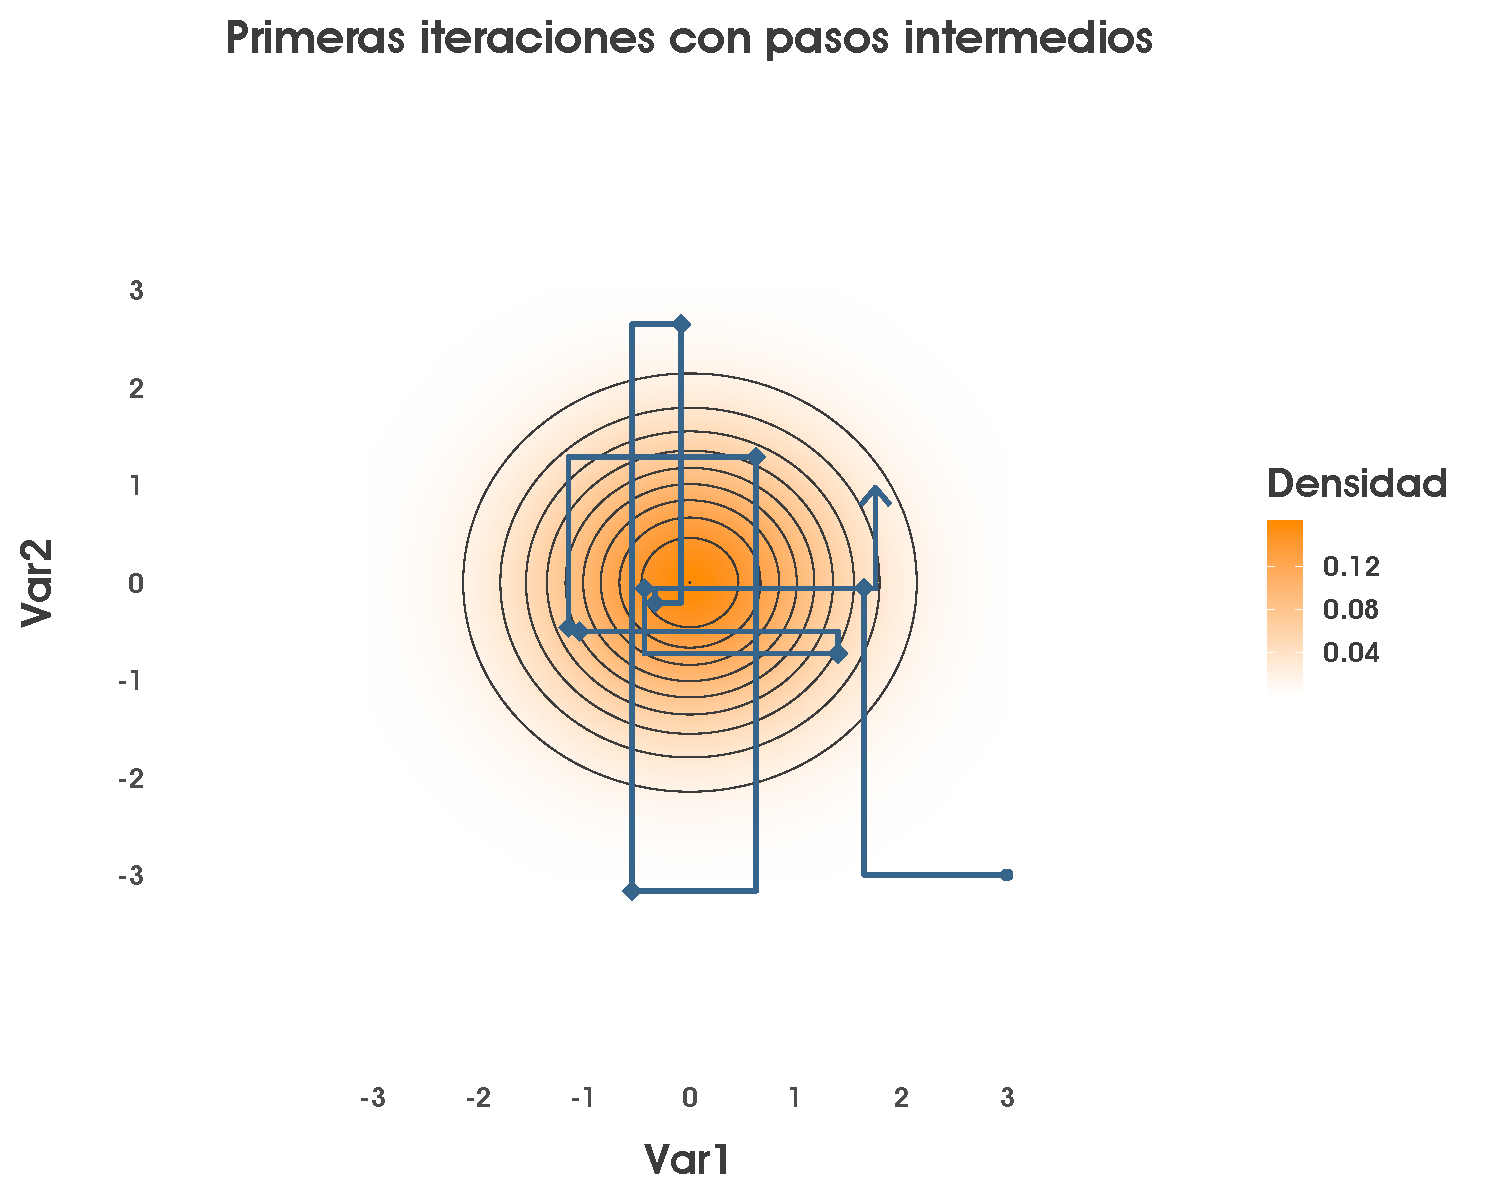
\includegraphics[width=\textwidth]{Figs/Bayes/Ejemplo_GS_A}
        \caption{El algoritmo consiste en dar pasos de Gibbs intermedios mediante las condicionales completas. Cada transición de Gibbs se señala como un cuadrado.}
    \end{subfigure}
    ~ 
    \begin{subfigure}{0.3\textwidth}
        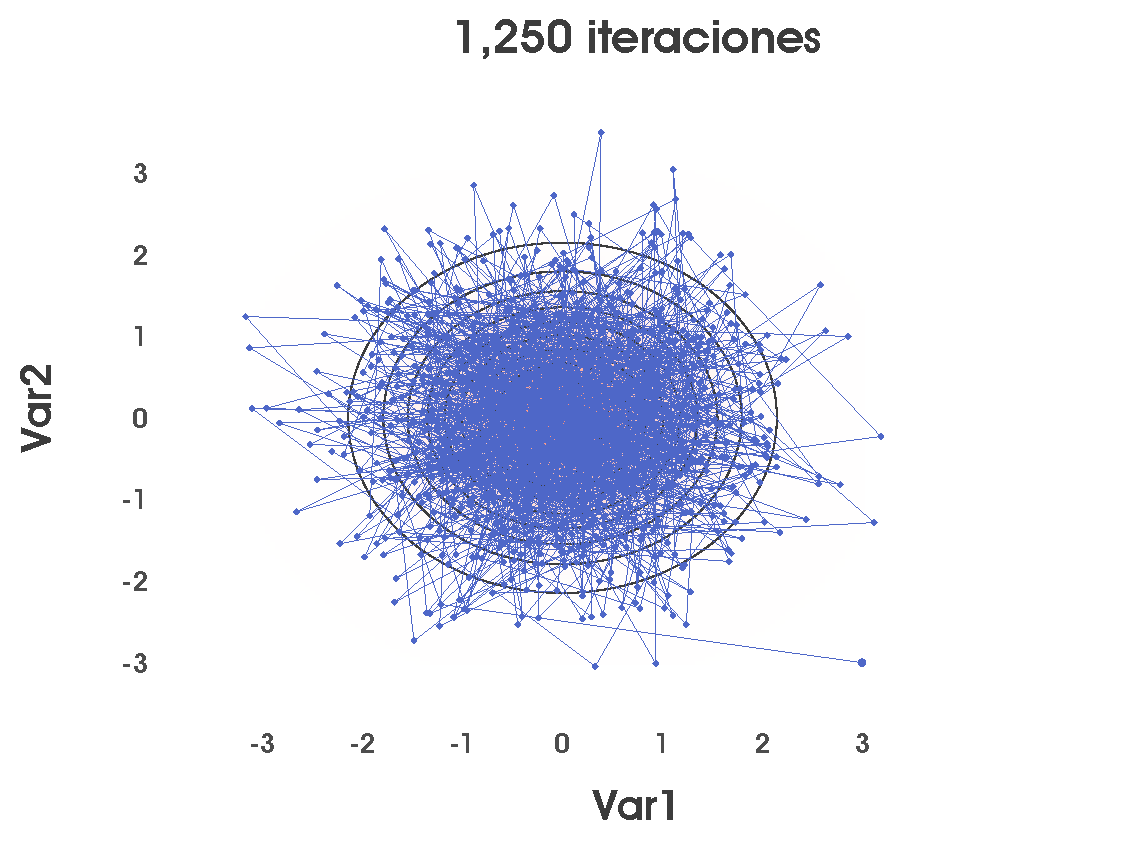
\includegraphics[width=\textwidth]{Figs/Bayes/Ejemplo_GS_B}
        \caption{Después de 1,250 transiciones, la cadena cubre completamente la región crítica.}
    \end{subfigure}
    ~
    \begin{subfigure}{0.3\textwidth}
        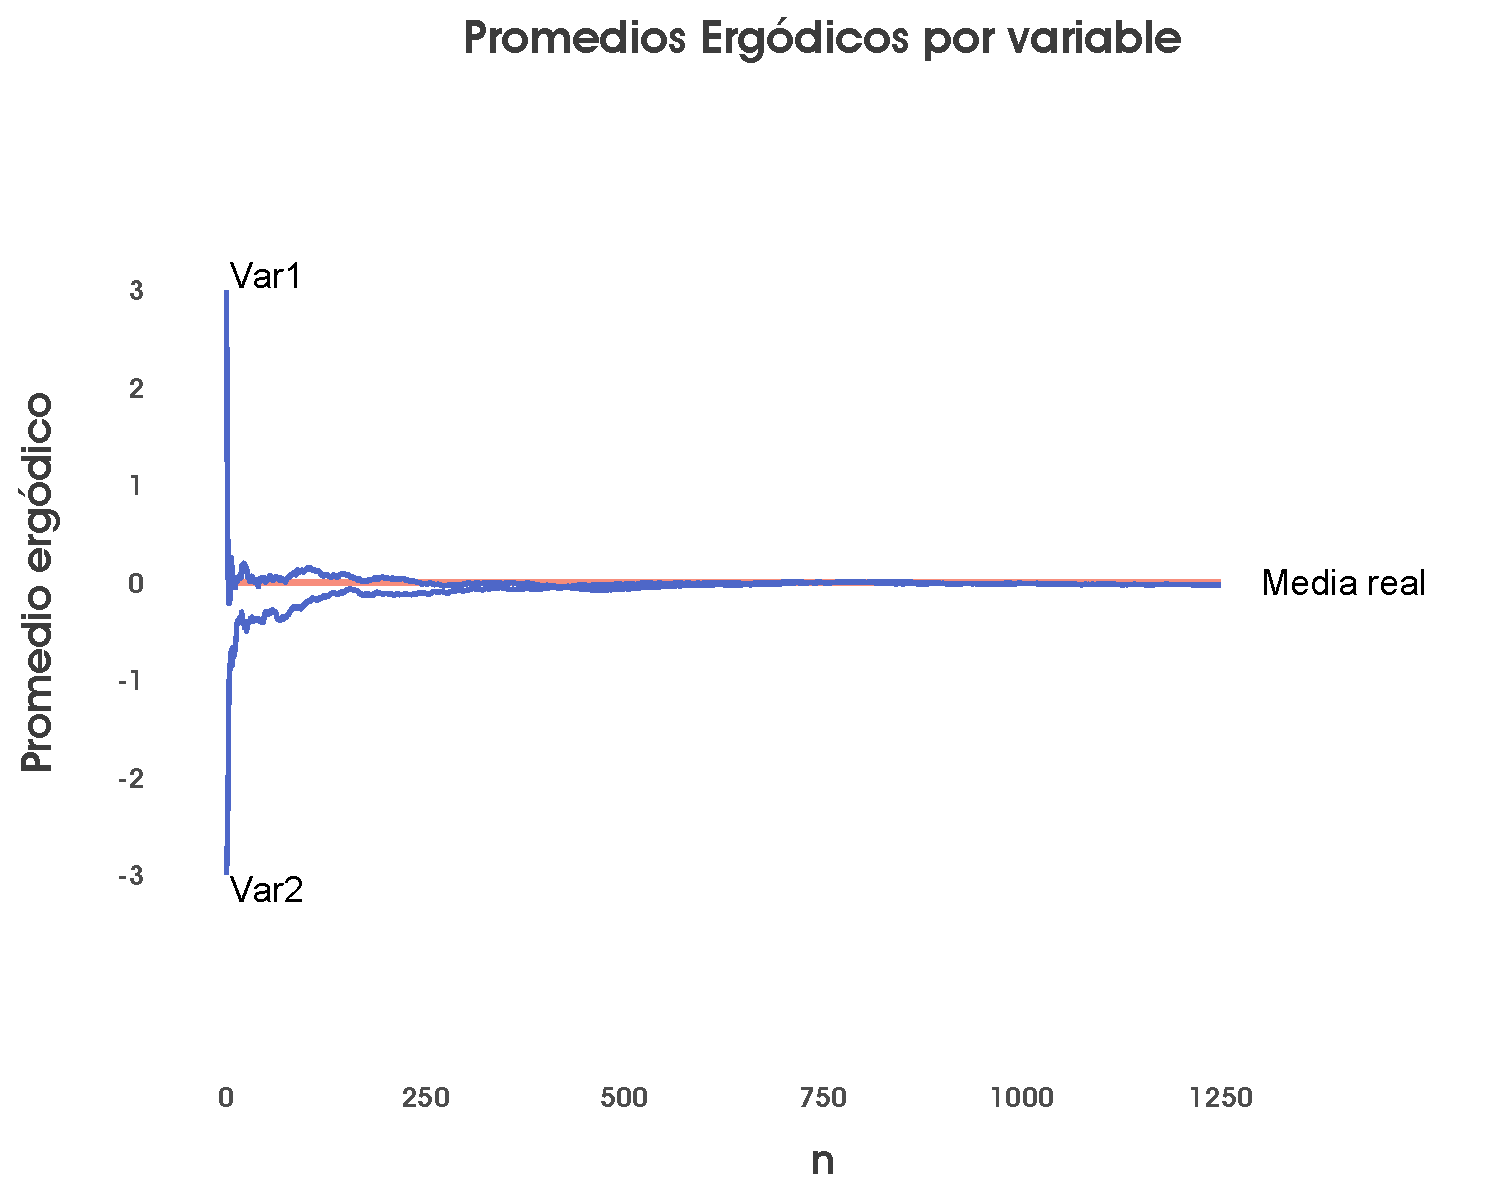
\includegraphics[width=\textwidth]{Figs/Bayes/Ejemplo_GS_C}
        \caption{Los promedios ergódicos convergen rápidamente a las medias teóricas, al rededor de la iteración 500. }
     \end{subfigure}
     \caption{Ilustración de una cadena de \textit{Gibbs Sampling} para una normal bivariada sin correlación. Fuente: elaboración propia.}\label{fig:GS_indep}
\end{figure}
 
En realidad, pocas veces contamos con tanta suerte como para tener completa independencia. Normalmente los parámetros que queremos simular están correlacionados entre sí. En la \textbf{Figura \ref{fig:GS_corr}} podemos ver cómo el \textbf{Gibbs Sampler} también se desempeña mucho mejor en este caso que RWM.\\
 
\begin{figure}[h]
    \centering
    \begin{subfigure}{0.3\textwidth}
        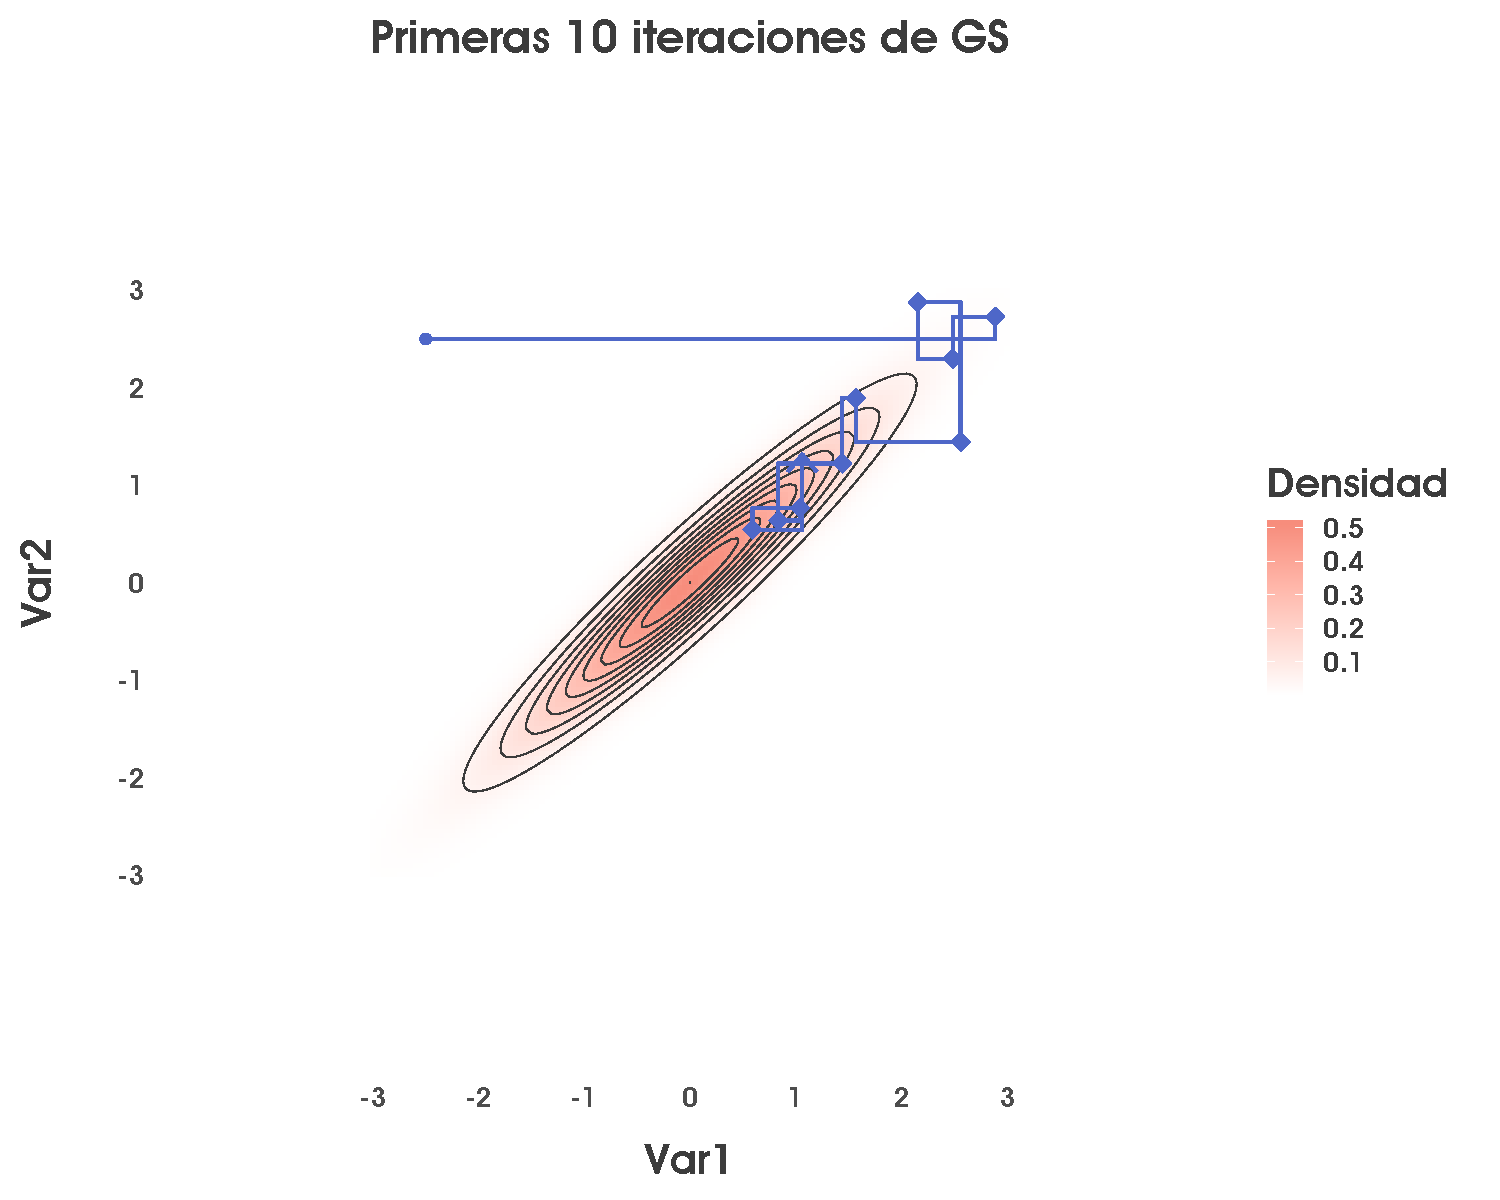
\includegraphics[width=\textwidth]{Figs/Bayes/Ejemplo_GS_Compara1}
    \end{subfigure}
    ~
    \begin{subfigure}{0.3\textwidth}
        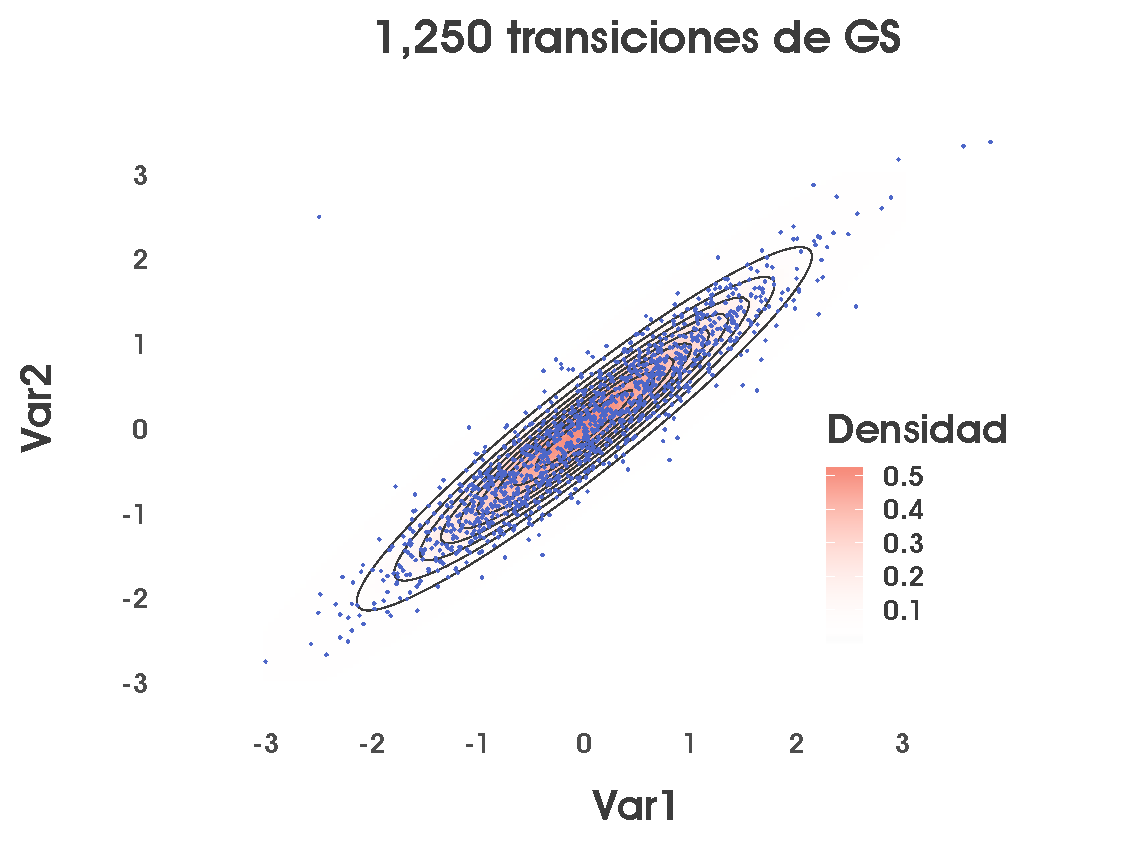
\includegraphics[width=\textwidth]{Figs/Bayes/Ejemplo_GS_Compara2}
    \end{subfigure}
    ~
    \begin{subfigure}{0.3\textwidth}
        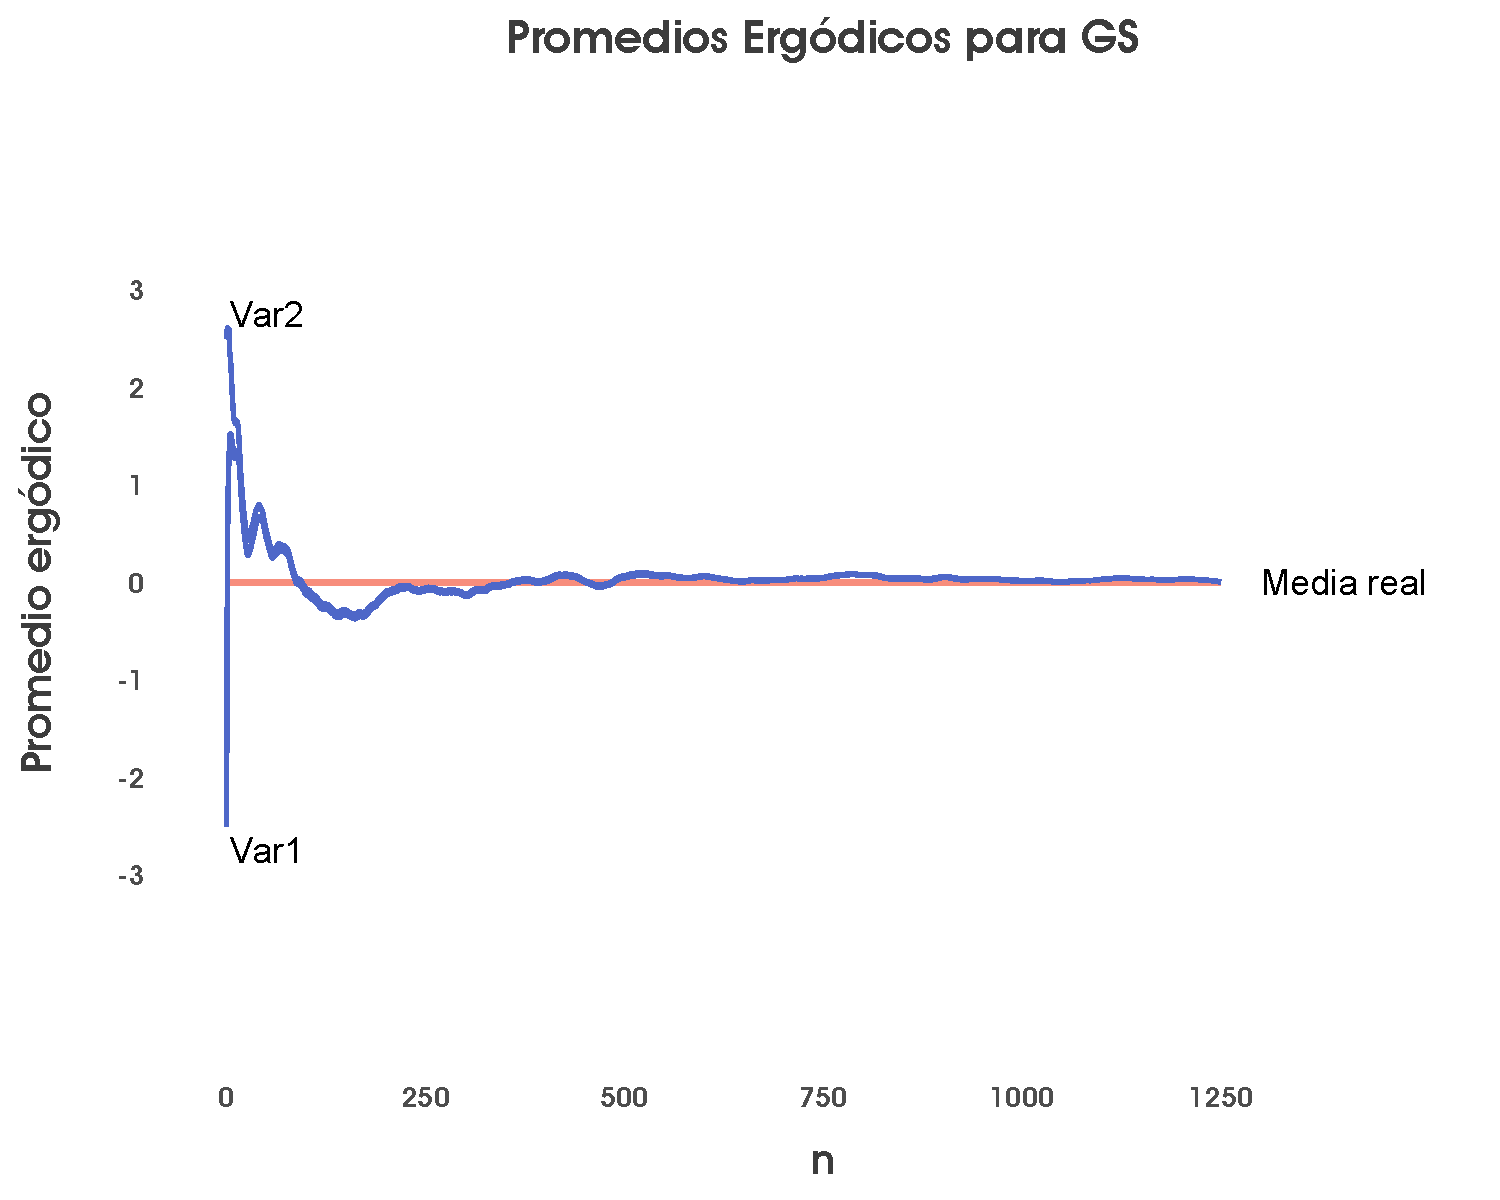
\includegraphics[width=\textwidth]{Figs/Bayes/Ejemplo_GS_Compara3}
    \end{subfigure}
    ~
    \begin{subfigure}{0.3\textwidth}
        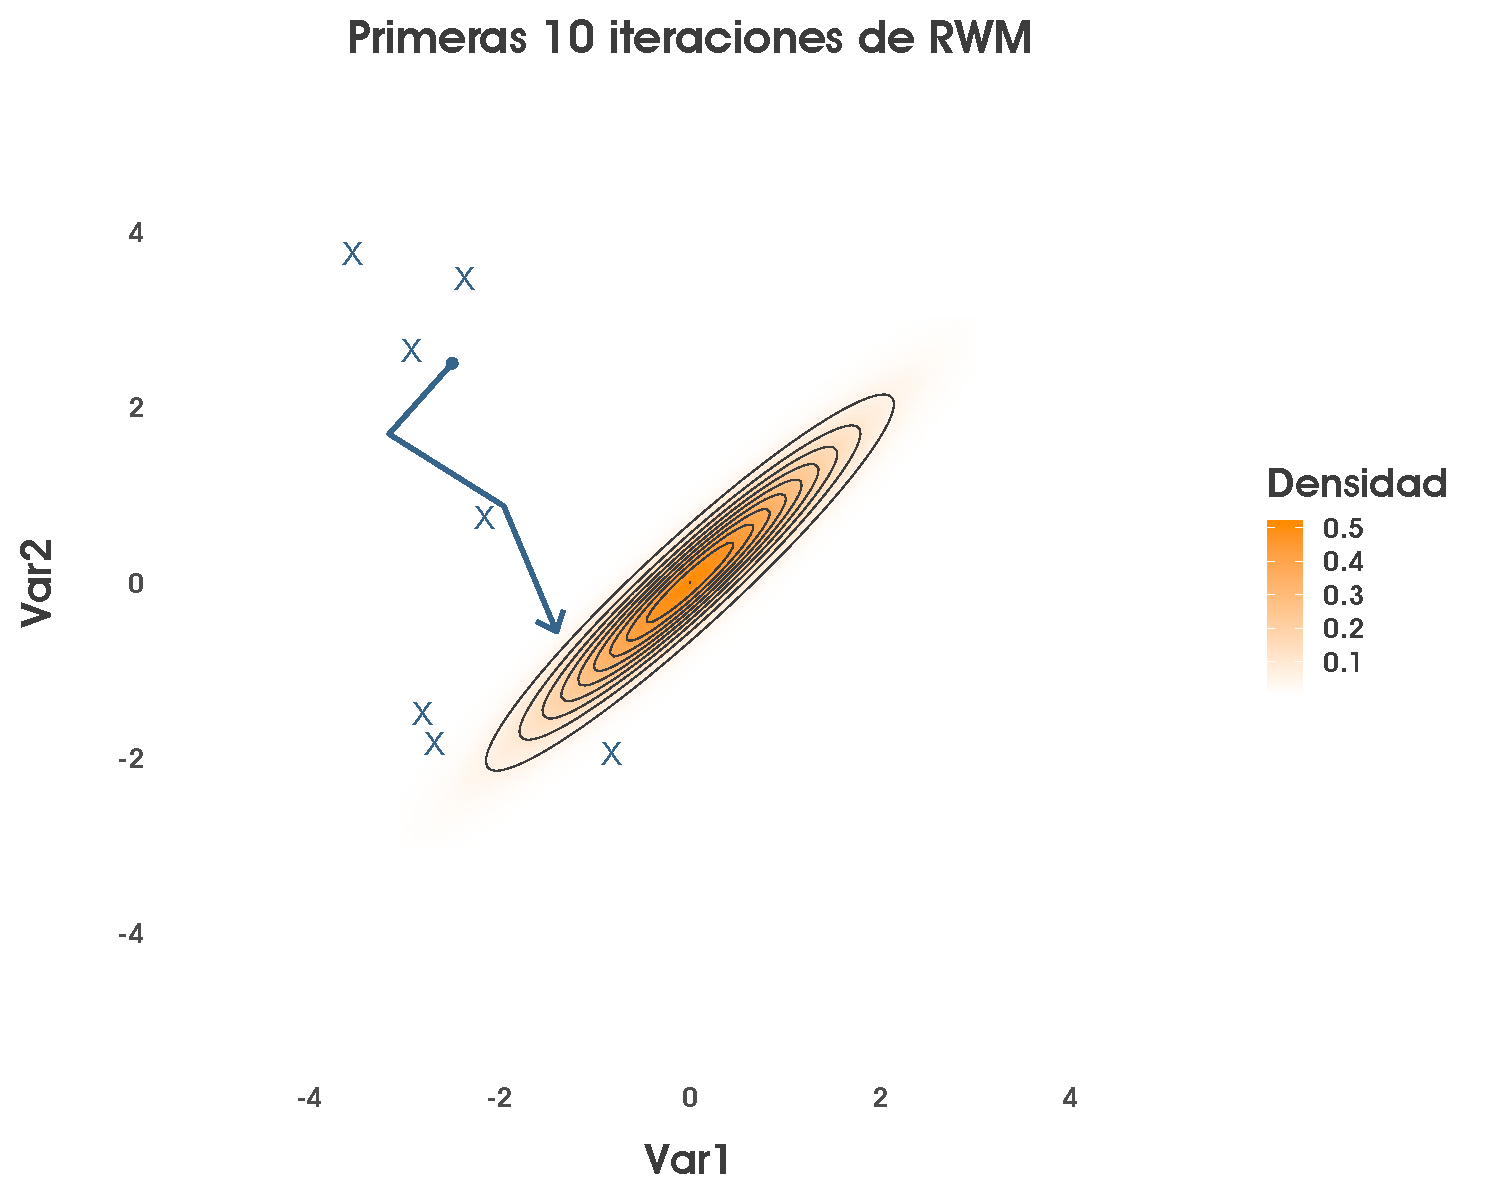
\includegraphics[width=\textwidth]{Figs/Bayes/Ejemplo_RWM_Compara2A}
    \end{subfigure}
    ~
    \begin{subfigure}{0.3\textwidth}
        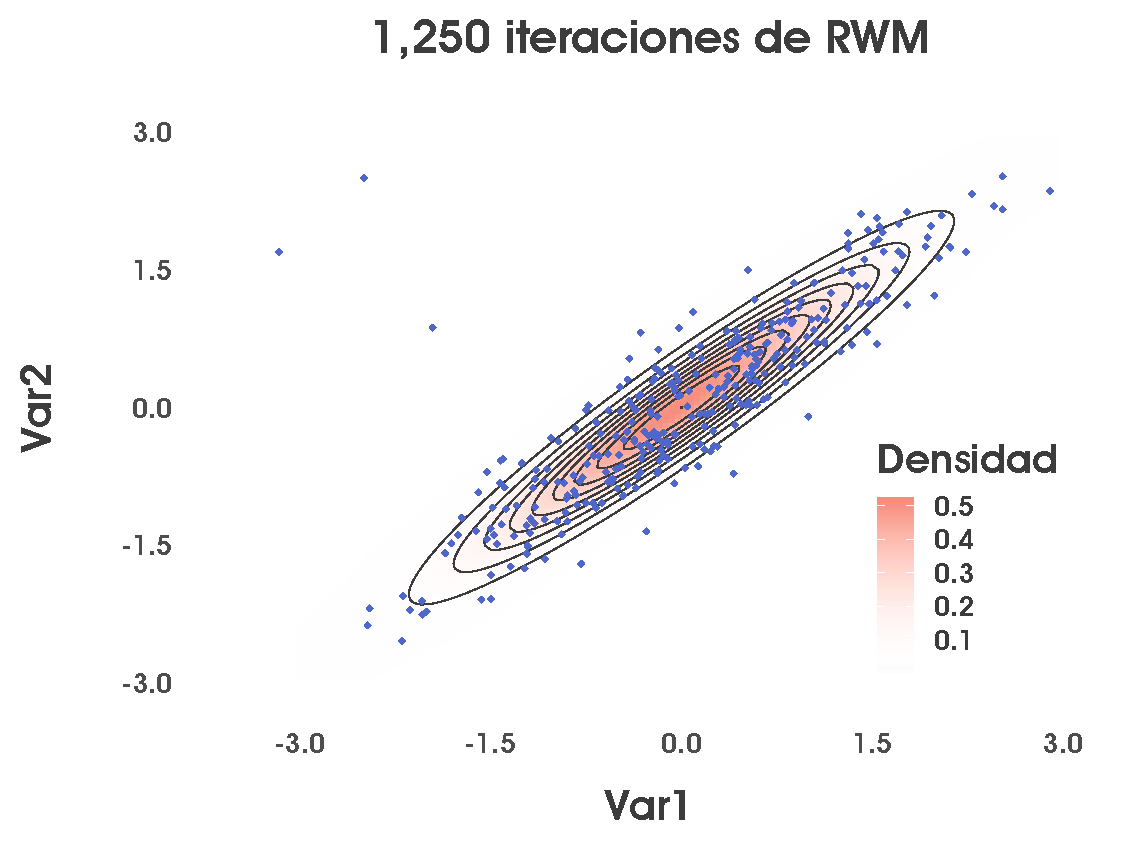
\includegraphics[width=\textwidth]{Figs/Bayes/Ejemplo_RWM_Compara2B}
    \end{subfigure}
    ~
    \begin{subfigure}{0.3\textwidth}
        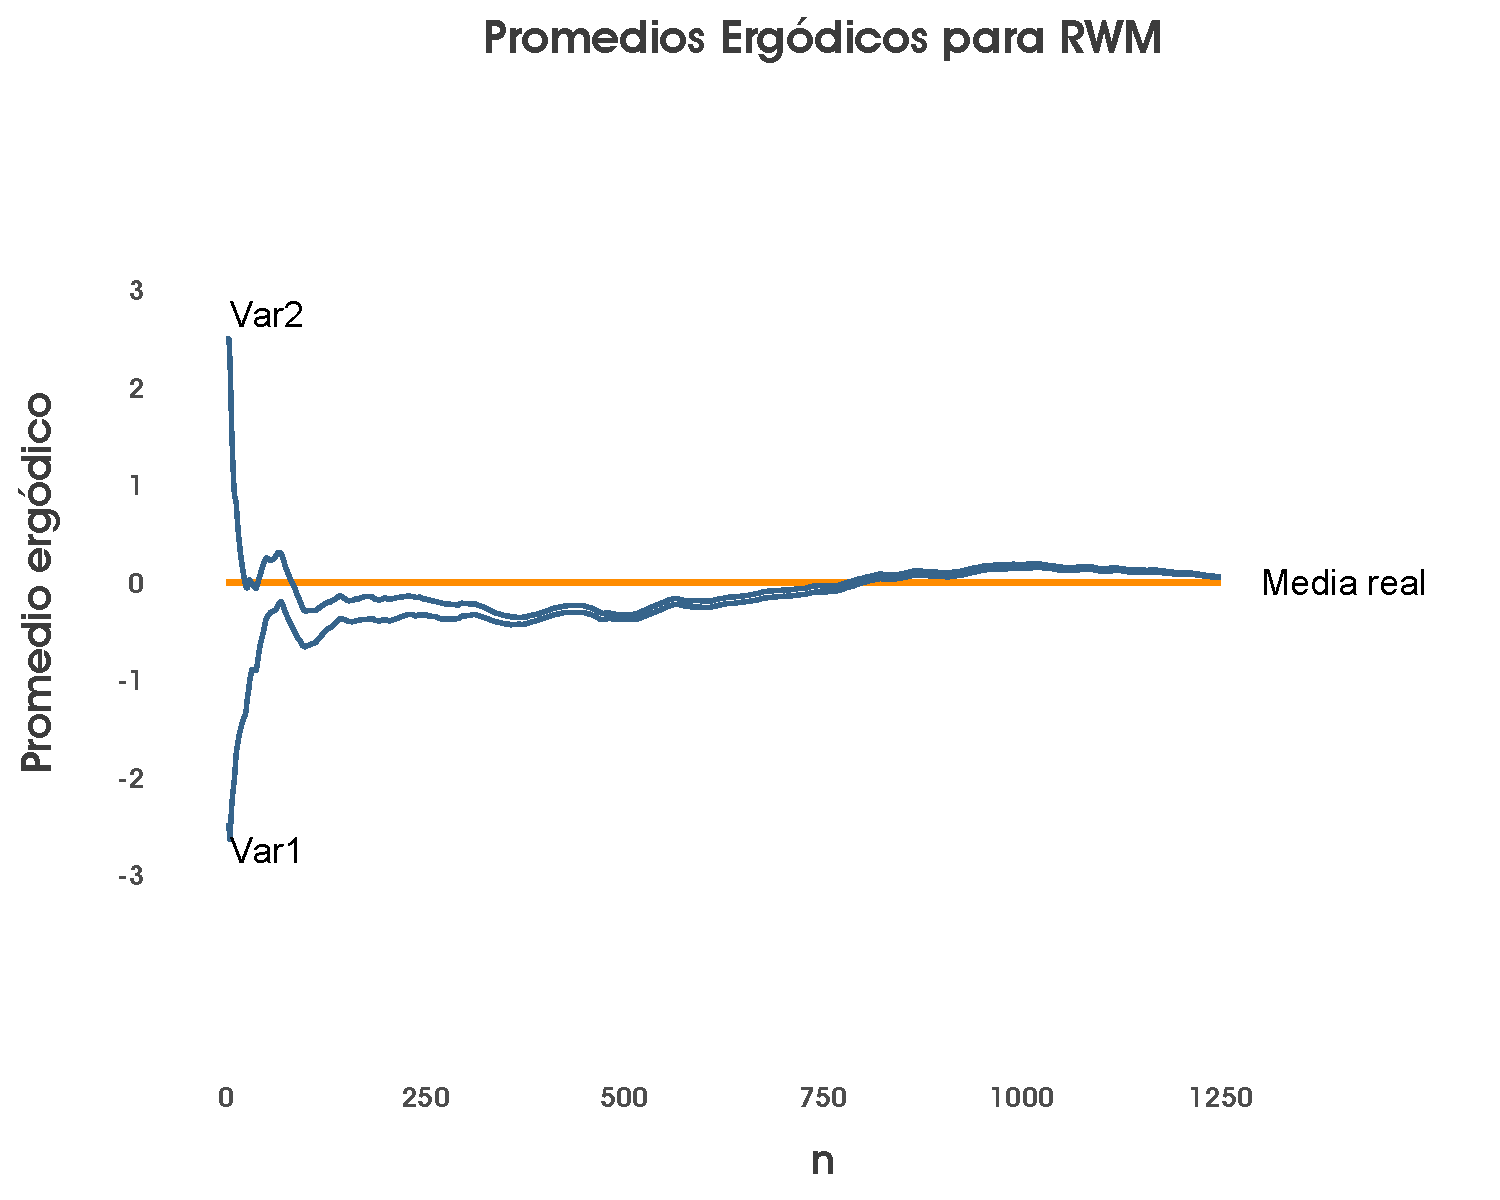
\includegraphics[width=\textwidth]{Figs/Bayes/Ejemplo_RWM_Compara2C}
    \end{subfigure}
    \caption{Comparación del \textit{Gibbs Sampler} (GS) con \textit{Random Walk Metropolis} (RWM) para simular de una normal bivariada de correlación 0.95. Las condicionales completas le permiten al GS llegar a la región crítica más rápidamente que al kernel uniforme de RWM que se retrasa en cada propuesta rechazada. Si comparamos todos los valores simulados después de 1,250 iteraciones vemos cómo aquellos de GS cubren de mejor manera la región crítica que los de RWM, mismos que se disturbaron ligeramente para presentar también los valores que se repiten por los rechazos. Asimismo, los promedios ergódicos convergen más rápidamente para GS que para RWM. Fuente: elaboración propia.}\label{fig:GS_corr}
\end{figure}

Por otro lado, si comparamos entre los dos casos del \textit{Gibbs sampler}, vemos que el desempeño se vio afectado al agregar correlación. Este es un fenómeno que se debe tener siempre presente: cuando la parametrización del modelo genera alta correlación entre los componentes, el algoritmo se hace más lento. El motivo es un equivalente al caso de un kernel de transiciones más estrecho. La correlación de los parámetros implica que las condicionales completas están muy concentradas, determinadas fuertemente por el valor actual; es decir, la simulación no puede generar un valor muy alejado del actual y el avance de la cadena es más lento.\\ 

Por ello, el \textit{Gibbs Sampler} puede sucumbir en la práctica ante problemas no triviales de alta correlación. Sabemos que convergerá, pero puede no hacerlo en un tiempo razonable, llegando a pasar cientos de miles de iteraciones antes de converger. Se pueden buscar parametrizaciones e implementaciones de Gibbs que mejoren el desempeño, pero como dice el \textcite{Stan17}, 
\begin{quote}
...incluso una implementación eficiente y escalable no resuelve el problema subyacente de que \textit{Gibbs sampling} no se desempeña bien con posteriores altamente correlacionadas. Finalmente nos dimos cuenta que necesitábamos un mejor muestreador, no una mejor implementación.
\end{quote}

Ese mejor muestreador se materealizó en el software \textit{Stan}--- nombrado así en honor al propio Stan Ulam--- cuya primera versión estable fue liberada en 2013 y que introduciré más adelante. Pero antes de hacerlo, quisiera detenerme en un tema que he omitido por ahora.\\

\subsection{Convergencia}

La convergencia de los promedios ergódicos que implica \eqref{eq:Teo_Erg_Conv_Prom} es la clave de un análisis de MCMC, pues nos permite aproximar los resúmenes inferenciales que necesitamos, tanto como nuestros recursos computacionales lo permitan. Sin embargo, como ya he mencionado, en un análisis bayesiano la única receta indica tener una muestra aleatoria de la distribución posterior. Si observamos con cuidado \eqref{eq:Teo_Erg_Conv_D}, vemos que la última simulación de la cadena es la que podemos considerar como proveniente de la distribución objetivo límite. Si quisiéramos una muestra de tamaño $N$, podríamos inicialmente pensar que necesitaríamos correr $N$ cadenas independientes.\\ 

Afortunadamente, en las cadenas de MCMC en general, la distribución límite es también lo que se conoce como \textit{distribución estacionaria} de la cadena de Markov. Esto quiere decir que el kernel de transición de la cadena mantiene estable la distribución de las simulaciones, una vez que se alcanza la distribución estacionaria \parencite{Neal93}. Esta característica estacionaria de la distribución límite implica que si reiniciamos la cadena una vez que se llega a la convergencia, podemos después de algún número de transiciones adicionales contar con otra observación prácticamente independiente proveniente de la misma distribución objetivo.\\ 

Por consiguiente, aunque los algoritmos de MCMC producen cadenas correlacionadas, es posible calcular un \textit{tamaño efectivo de muestra} que aproxima el tamaño de una muestra aleatoria auténticamente independiente proveniente de la distribución objetivo cuyas estimaciones equivaldrían a las que hacemos con la muestra simulada. Los detalles de cómo se calcula dicha estadística puede consultarse en \textcite{Gelman13}.\\ 

Por lo anterior, usualmente solo se conservan las simulaciones cada $m$ transiciones de manera que la correlación entre ellas sea lo más cercana a cero posible. Buscaríamos descartar aquellas simulaciones que, debido a la correlación, no están aportando realmente mayor información sobre la distribución objetivo. Con este \textit{adelgazamiento} de la cadena se busca ahorrar espacio de memoria en la computadora y conservar solo las simulaciones que aportan \textit{nueva} información y aumentan el tamaño efectivo de muestra.\\ 

En este sentido, la forma usual de aplicar la única receta de la inferencia bayesiana mediante MCMC se resume de la manera siguiente: 

\begin{enumerate}
\item Elegir un número $c$ de cadenas para simular.
\item Iniciar cada cadena en un punto distinto y disperso del espacio parametral. 
\item Correr de manera independiente las $c$ cadenas hasta que ``alcancen la convergencia''. 
\item Una vez que se considera que las cadenas convergieron, se desechan las transiciones iniciales que constituyen el \textit{periodo de calentamiento}. 
\item Se \textit{adelgaza} cada cadena conservando las simulaciones solo cada $m$ transiciones de manera que la correlación sea baja. 
\item Se continúan realizando simulaciones después del calentamiento y el adelgazamiento hasta obtener una muestra ``lo suficientemente grande''.  
\end{enumerate}

El número de cadenas se puede elegir en función del número de procesos paralelos que la computadora puede realizar para aprovechar la eficiencia que implica el cómputo paralelo. Usualmente se corren 3, 4 o 5 cadenas. Por su parte, seleccionar el espaciamiento $m$ de las cadenas normalmente implica realizar gráficos de autocorrelación para algunas pruebas preliminares cuyo objetivo es también determinar la convergencia del algoritmo. En realidad, el punto más delicado es precisamente este último, declarar la convergencia.\\ 

Desafortunadamente, los teoremas ergódicos son asintóticos, por lo que solo se garantiza la convergencia en el infinito. Aunque hay cotas para los errores, normalmente no son muy útiles, salvo algunos casos \parencite{SmithRoberts93}. Por ello, en la práctica se han desarrollado diferentes técnicas de diagnóstico de convergencia. Sin embargo, ninguna puede garantizarnos totalmente que la cadena ya haya convergido. Entonces, es recomendable considerar diferentes técnicas para disminuir la probabilidad de pasar por alto algún problema de convergencia. Una vez que estamos satisfechos con las pruebas de convergencia, podemos utilizar todas las simulaciones como una sola muestra que caracteriza la distribución posterior y realizar las estimaciones de Monte Carlo necesarias.\\

La primera técnica ya la he utilizado en los ejemplos de RWM y Gibbs: graficar los promedios ergódicos para diferentes variables o resúmenes inferenciales para observar en qué punto se estabilizan. La segunda es precisente iniciar en puntos dispersos del espacio parametral para evitar que las cadenas exploren solo una parte del espacio y, por ejemplo, queden atrapadas en una sola moda cuando la distribución posterior pueda ser multimodal. Al mismo tiempo, tener diferentes cadenas nos permite comparar las estimaciones dentro de cada cadena así como a través de las cadenas. Un ejemplo de promedios ergódicos para 4 cadenas de \textit{Gibbs Sampler} (GS) iniciadas en puntos dispersos del espacio parametral puede verse en la \textbf{Figura \ref{fig:Conv_Prom_Erg}}.\\ 

\begin{figure}[h]
	\centering
	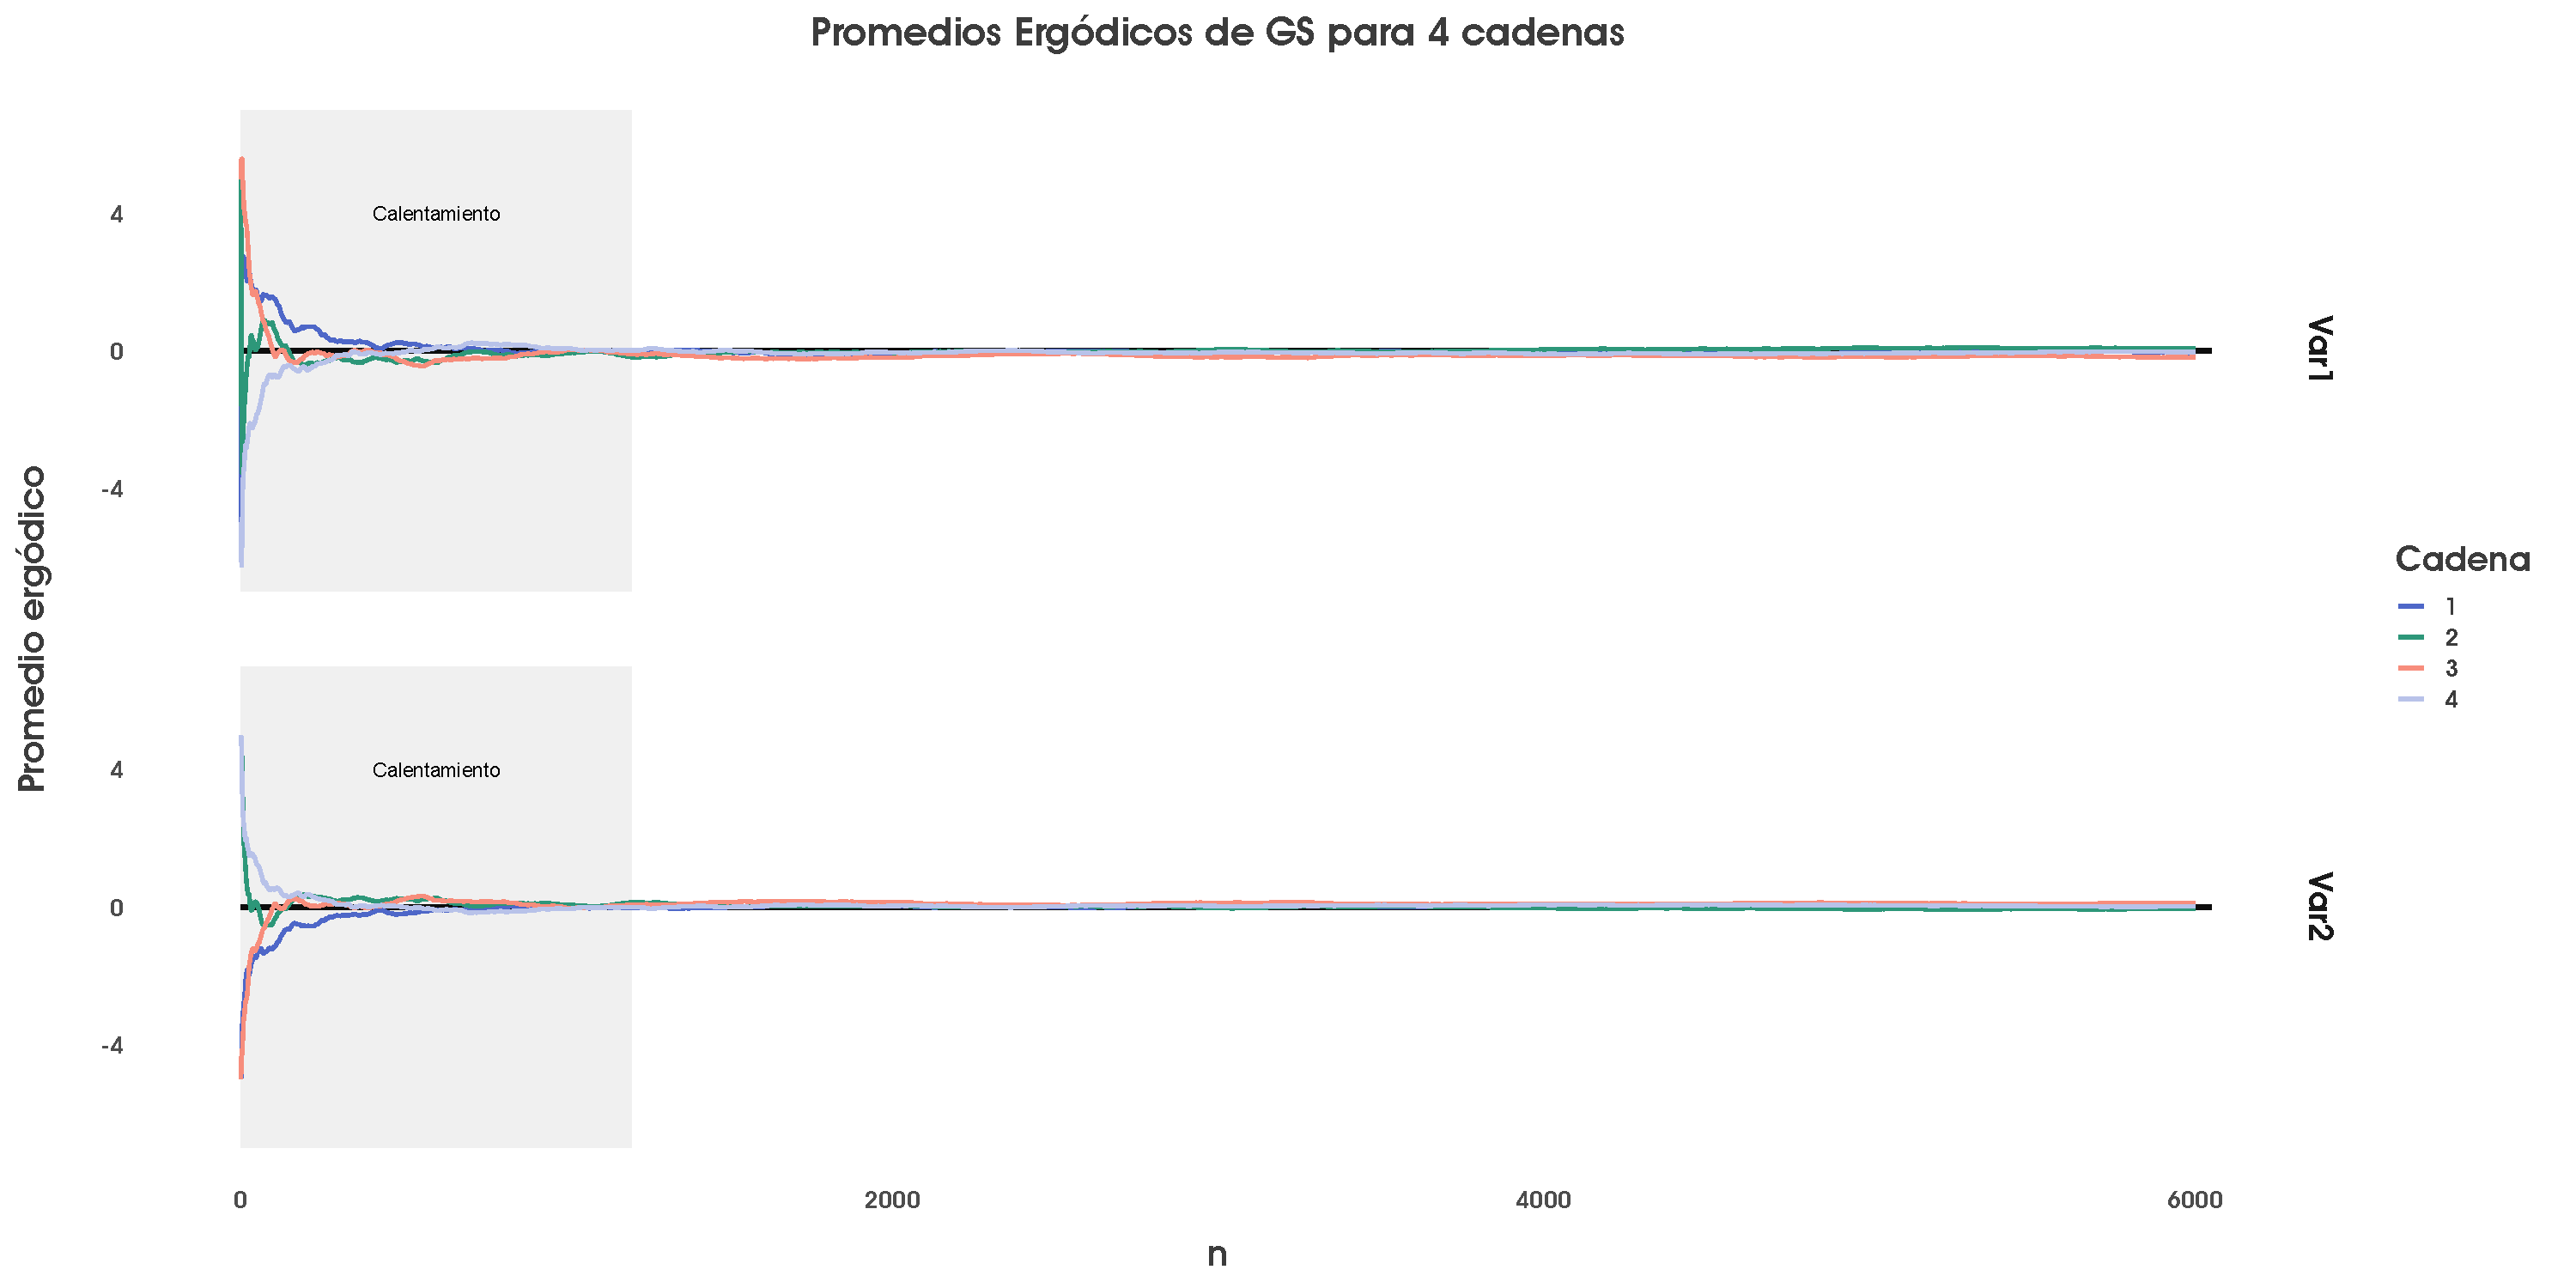
\includegraphics[width=0.9\textwidth]{Figs/Bayes/Ejemplos_Convergencia_Prom_Erg}
	\caption{Ilustración de la convergencia de dos promedios ergódicos para 4 cadenas de \textit{Gibbs Sampling} iniciadas en puntos dispersos del espacio parametral. Vemos cómo las estimaciones de distintas cadenas se estabilizan y mezclan. Esto ayuda a detectar la fase de calentamiento. Fuente: elaboración propia.}
	\label{fig:Conv_Prom_Erg}	
\end{figure}

En el fondo, hay dos características que se buscan para declarar la convergencia \parencite{Gelman13}. Queremos que las cadenas lleguen a la estacionariedad, pues la distribución límite es también estacionaria. Las estimaciones deben estabilizarse. También, y dicho de manera coloquial, buscamos que las cadenas \textit{mezclen} bien. Es decir, que las estimaciones para cada cadena sean parecidas a las estimaciones de todas las cadenas en su conjunto. Por ello un buen algoritmo de MCMC buscará recorrer y explorar todas las regiones críticas de la distribución objetivo \parencites{Neal93,Betancourt18}.\\ 

Uno de los diagnósticos visuales más utilizados son los llamados gráficos de oruga o \textit{trace plots}. En ellos se grafica la secuencia de iteraciones, es decir en el eje $x$ se encuentra el número de iteración y en el eje $y$ el valor de la cadena en dicha iteración. Si las cadenas son estacionarias entonces el gráfico saltará de un punto a otro dentro de un rango de valores que determinan la región crítica. Si las cadenas mezclan bien, entonces las diferentes secuencias estarán oscilando en la misma región crítica, intercalándose. El \textit{trace plot} del ejemplo de esta sección puede verse en la \textbf{Figura \ref{fig:Conv_Trace_Inicial}}. También podemos ver en la \textbf{Figura \ref{fig:Conv_Trace_Final}}, el gráfico correspondiente a las iteraciones válidas para cada cadena, es decir, después del descarte del periodo de calentamiento y el espaciamiento para evitar la correlación.\\

\begin{figure}[h]
	\centering
	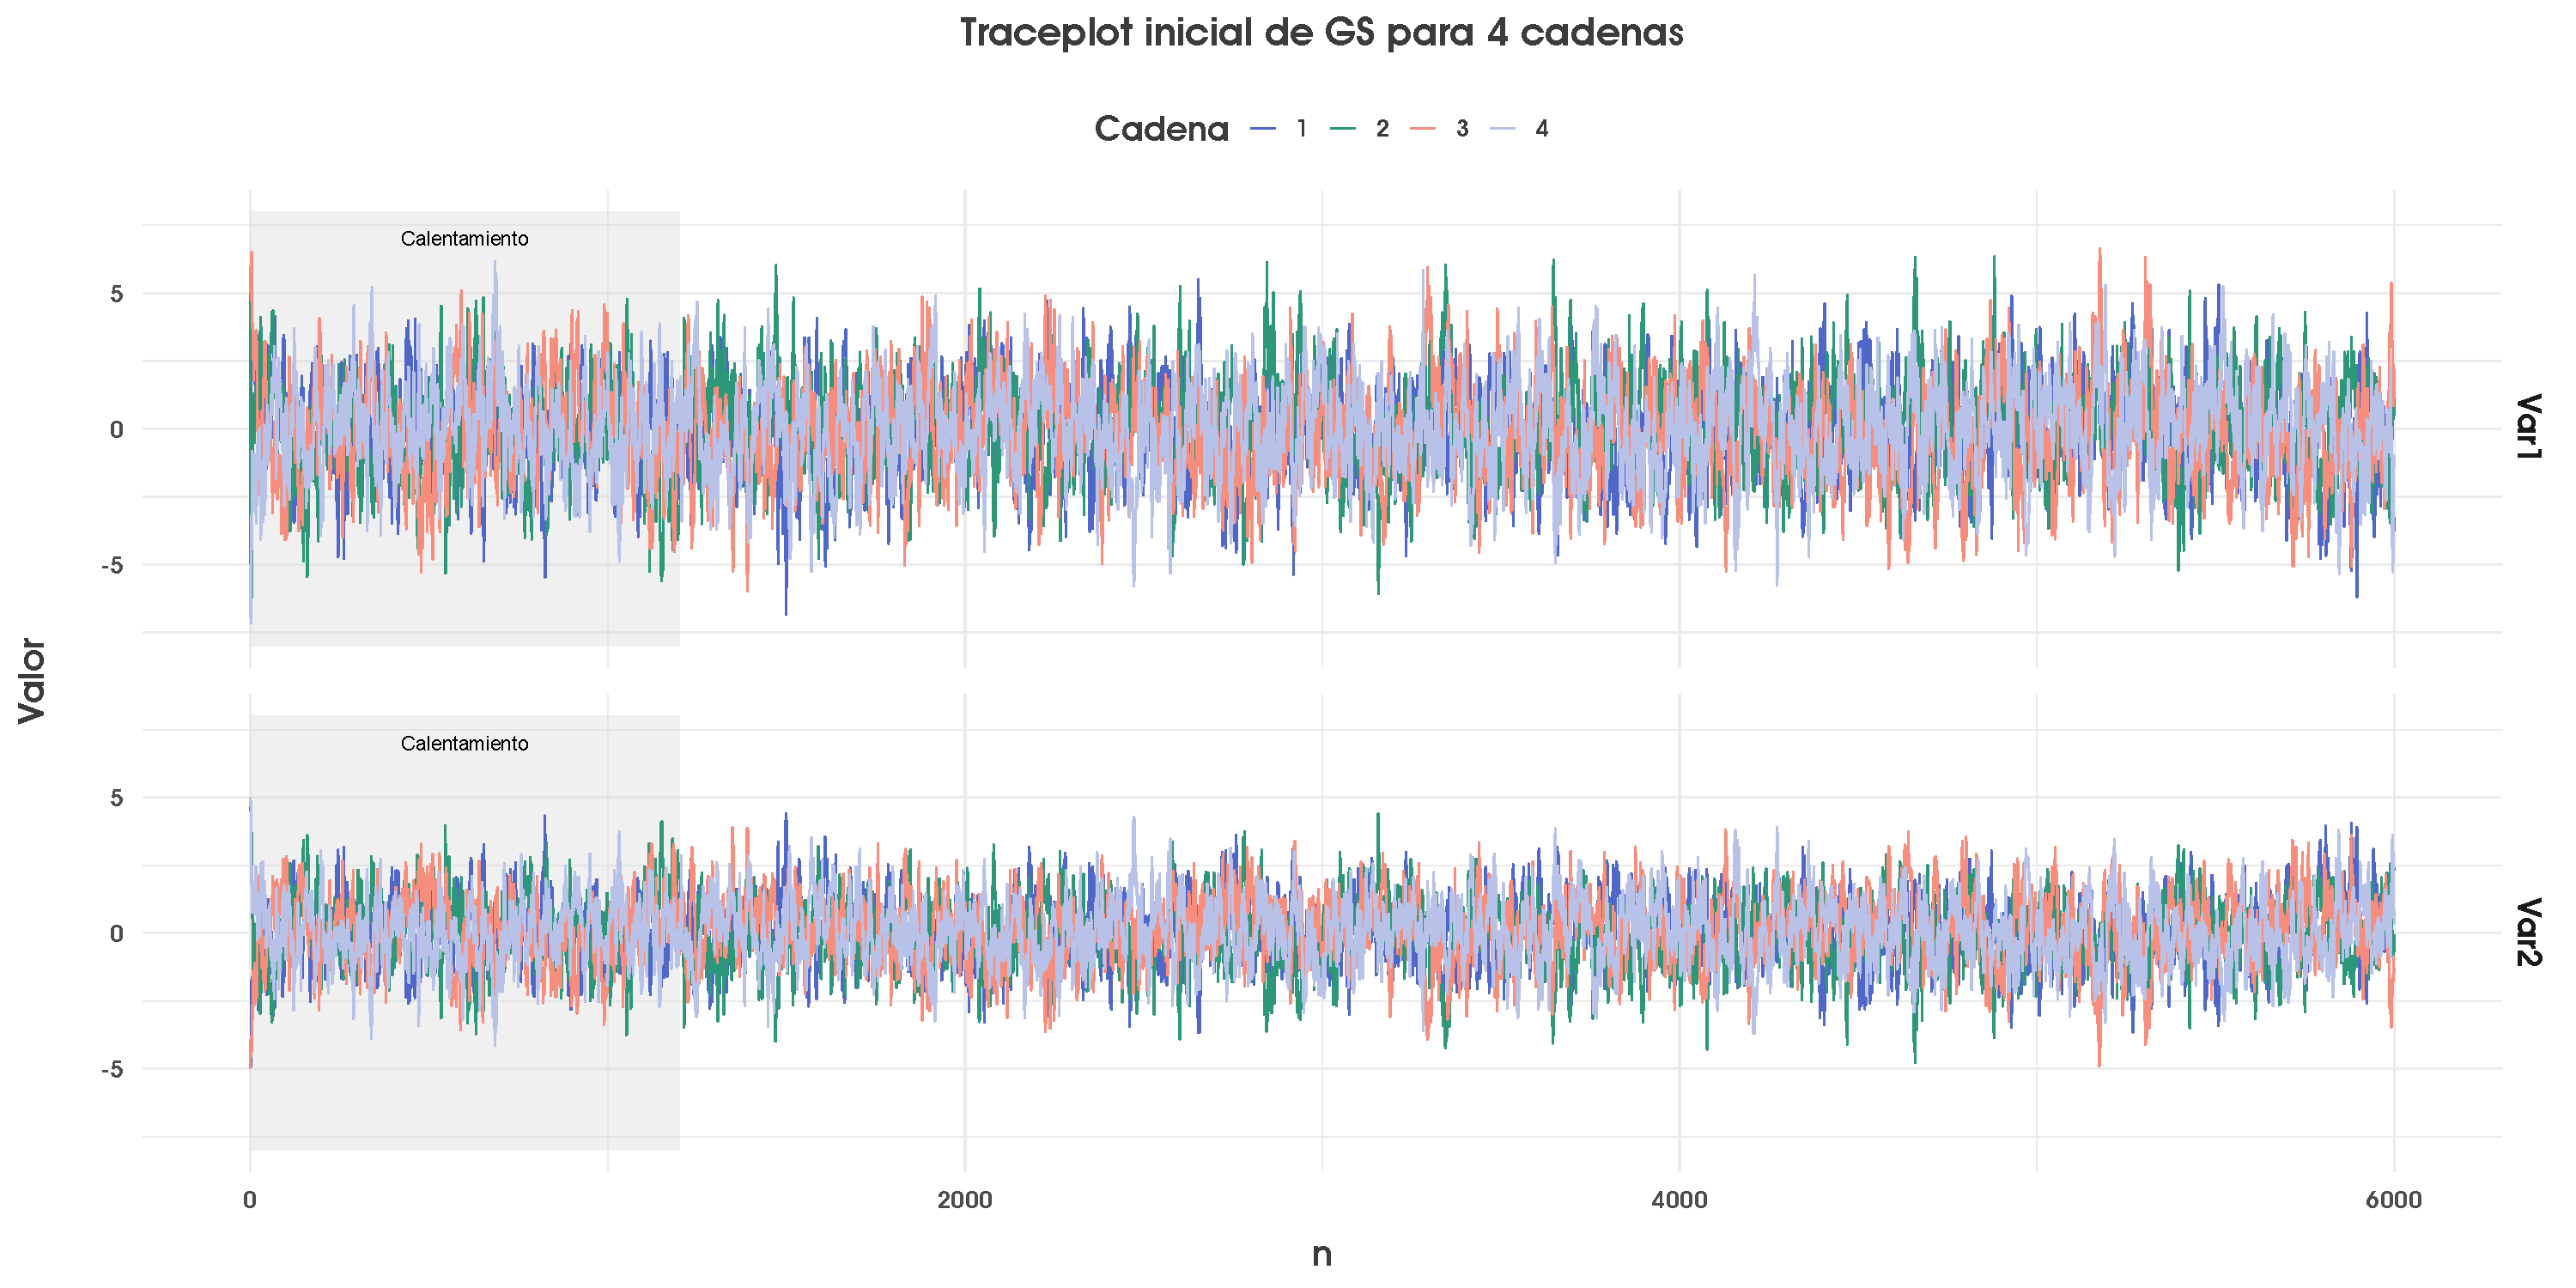
\includegraphics[width=0.9\textwidth]{Figs/Bayes/Ejemplos_Convergencia_Traceplot_Inicial}
	\caption{Ilustración de un \textit{trace plot} para las 4 cadenas de \textit{Gibbs Sampling}. Vemos el comportamiento de oruga, al rededor de una banda de valores. Fuente: elaboración propia.}
	\label{fig:Conv_Trace_Inicial}	
\end{figure}

\begin{figure}[h]
	\centering
	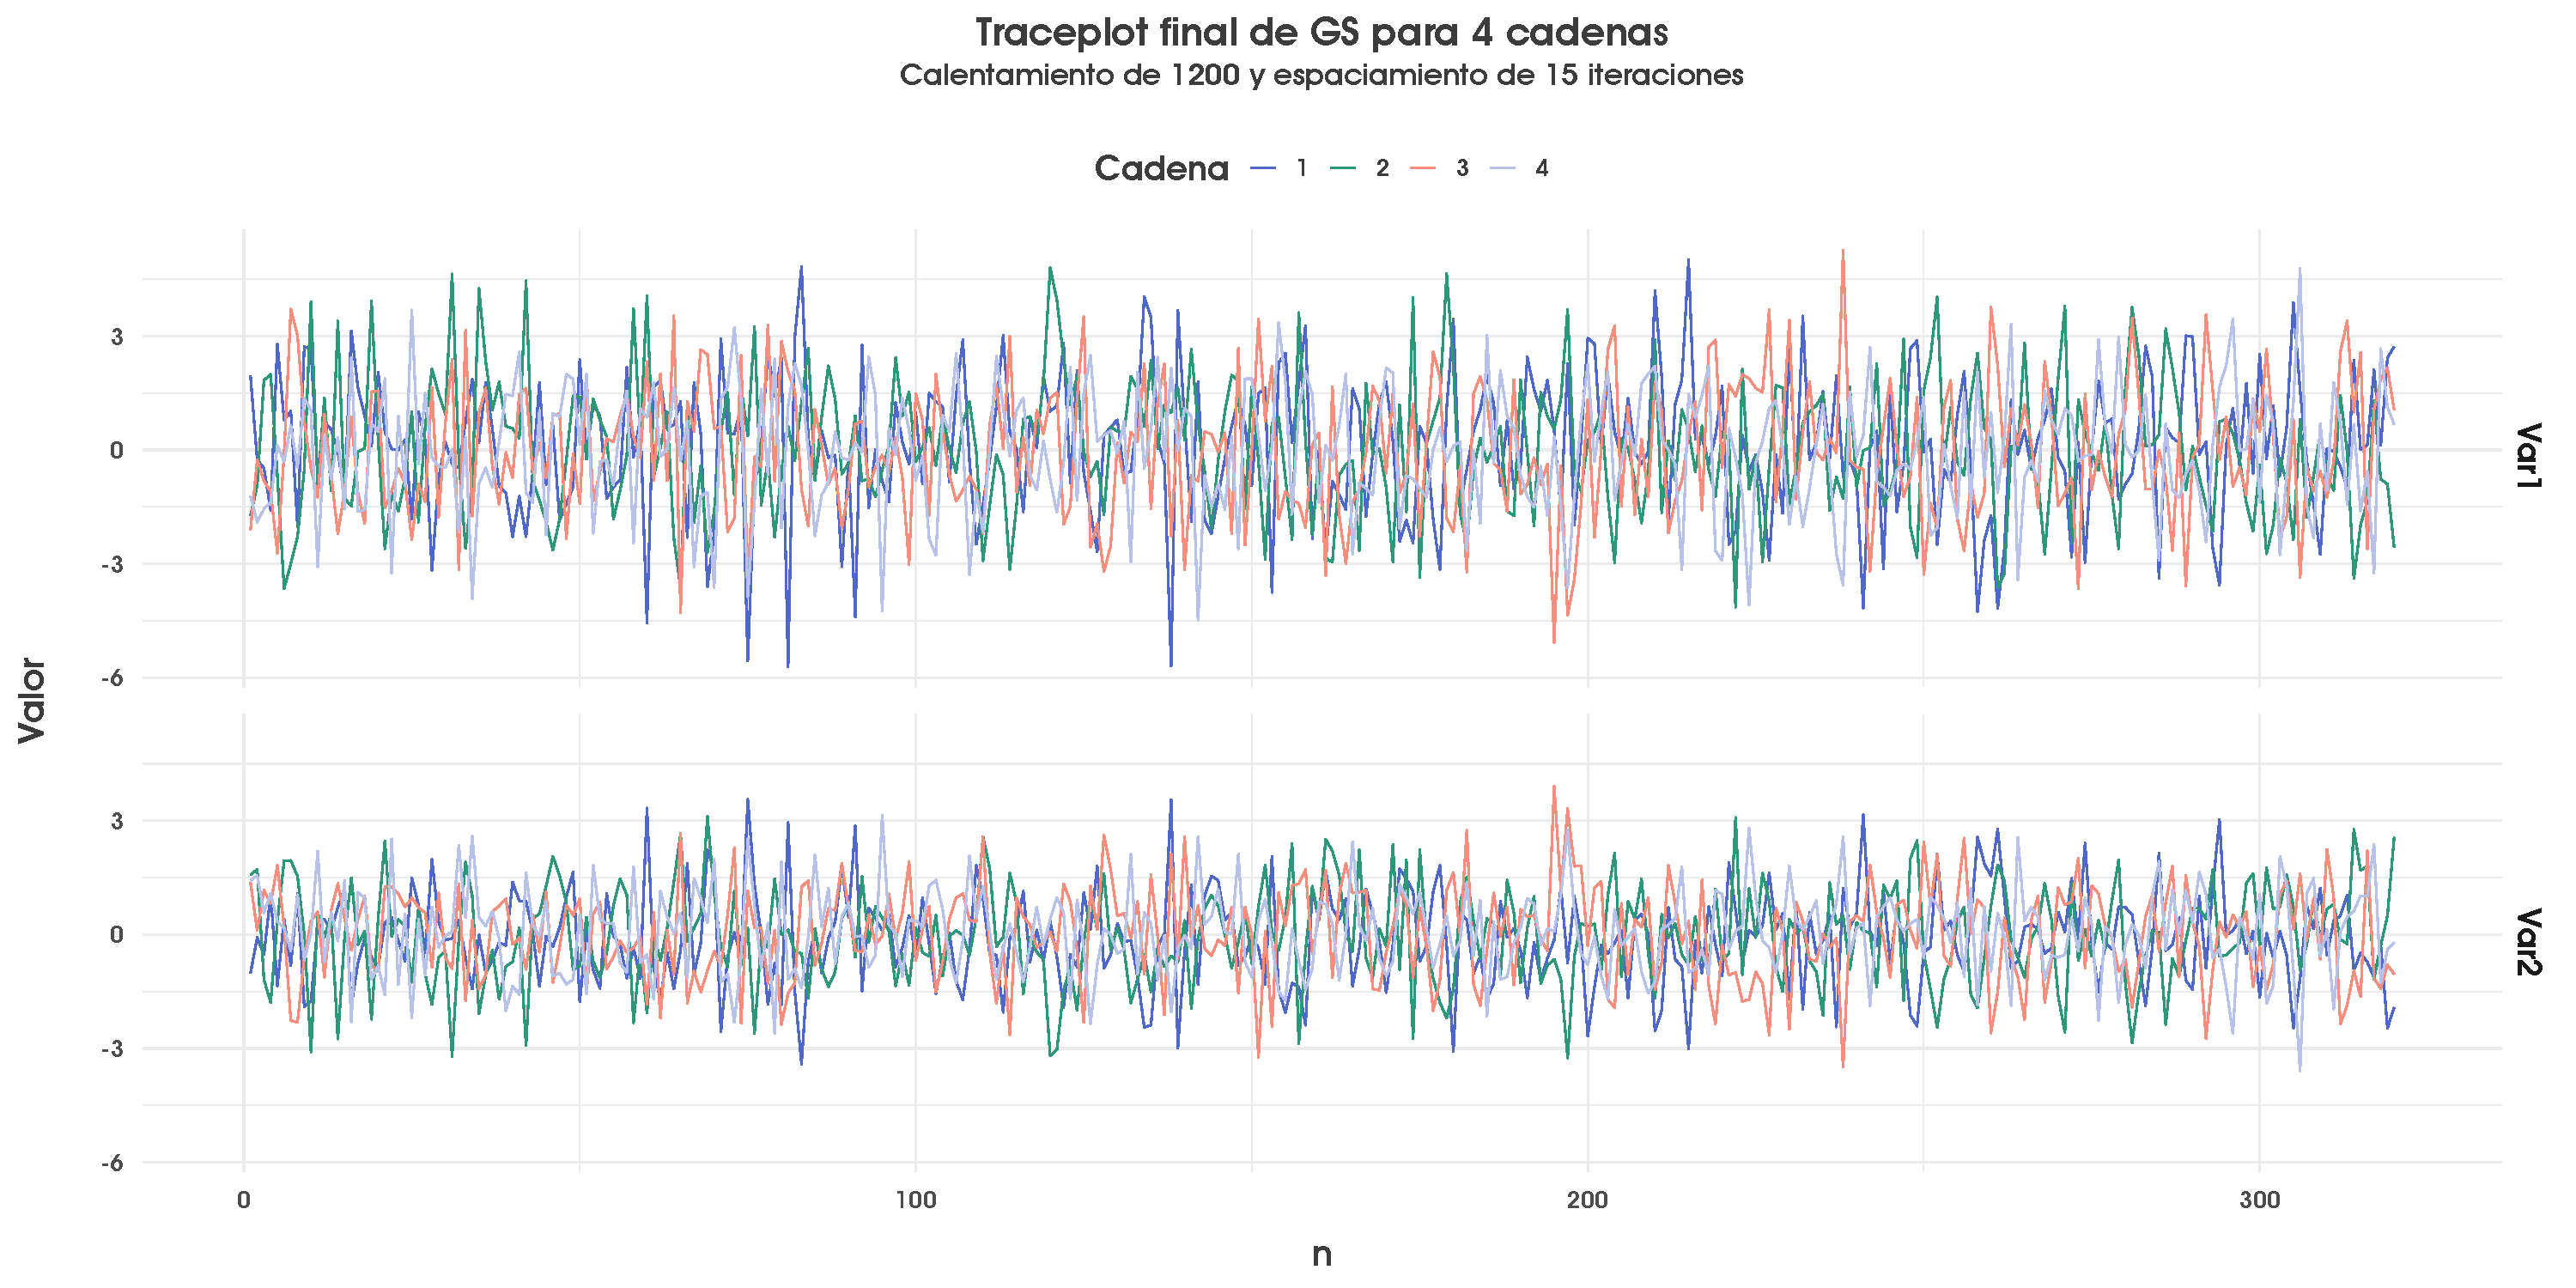
\includegraphics[width=0.9\textwidth]{Figs/Bayes/Ejemplos_Convergencia_Traceplot_Final}
	\caption{Ilustración de un \textit{trace plot} para las 4 cadenas de \textit{Gibbs Sampling} considerando solo las iteraciones válidas. Fuente: elaboración propia.}
	\label{fig:Conv_Trace_Final}	
\end{figure}

En este caso, el ejemplo es lo suficientemente sencillo para permitirnos un adelgazamiento de 8. La reducción en la autocorrelación que esto tiene se puede apreciar en la \textbf{Figura \ref{fig:Conv_Autocorr}}. En la práctica el adelgazamiento suele ser más chico.\\ 

\begin{figure}[h]
    \centering
    \begin{subfigure}{0.45\textwidth}
        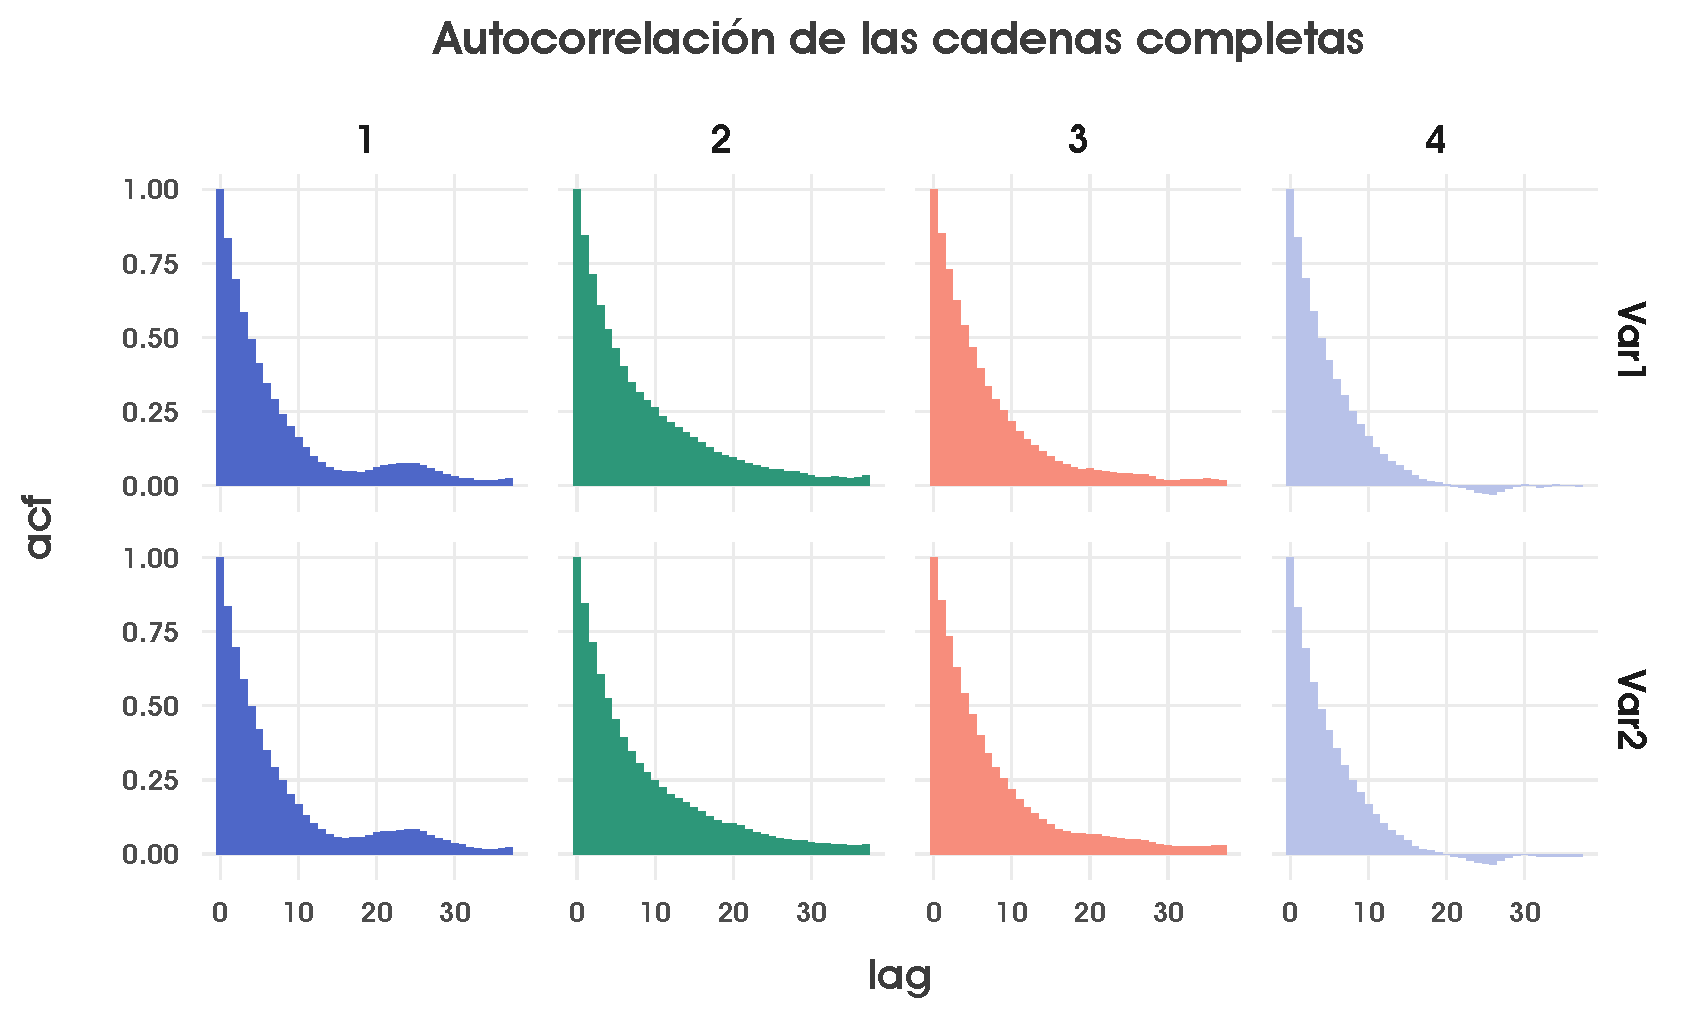
\includegraphics[width=\textwidth]{Figs/Bayes/Ejemplos_Convergencia_Autocorr_Completas}
    \end{subfigure}
    ~ 
    \begin{subfigure}{0.45\textwidth}
        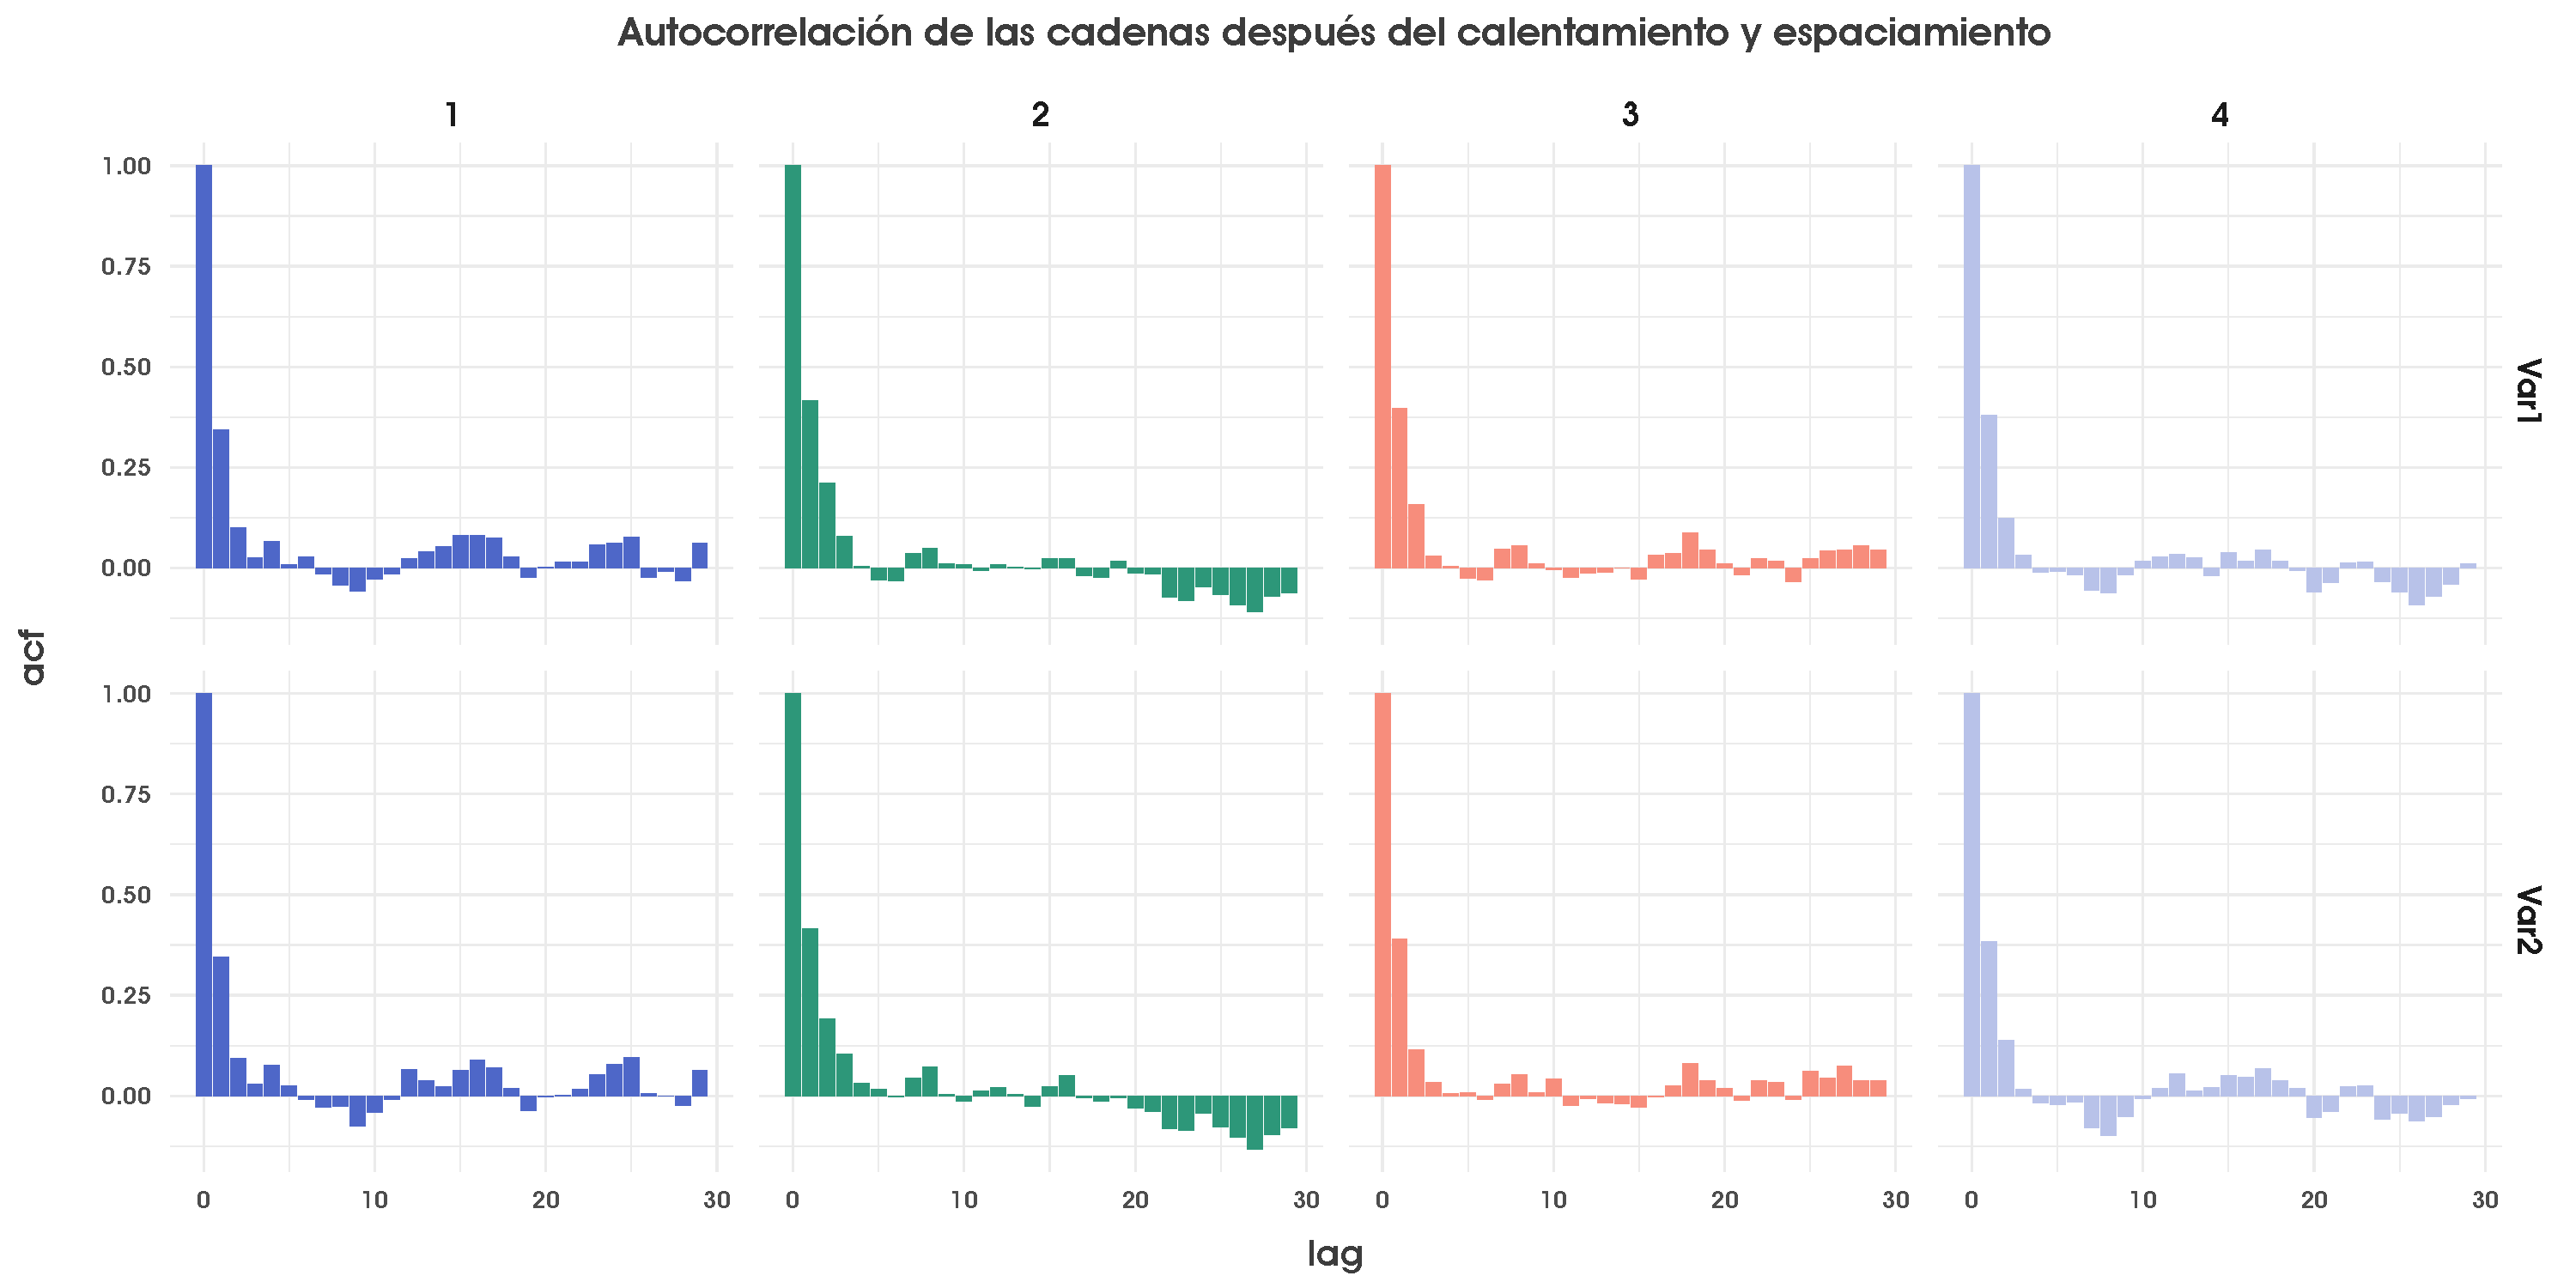
\includegraphics[width=\textwidth]{Figs/Bayes/Ejemplos_Convergencia_Autocorr_Final}
    \end{subfigure}
    \caption{Gráficos de autocorrelación para las 4 cadenas de \textit{Gibbs Sampling} antes y después de realizar un adelgazamiento de 8. Fuente: elaboración propia.}\label{fig:Conv_Autocorr}
\end{figure}

Otro diagnóstico gráfico es el de comparar histogramas o densidades estimadas para varios parámetros y resúmenes inferenciales y verificar que estos son estables--- comparándolos para la primera mitad de la muestra y para la segunda, por ejemplo--- y mezclan bien--- los gráficos para las diferentes cadenas se parecen al gráfico de todas juntas---. Para el ejemplo, vemos la comparación de los histogramas de cada cadena con el histograma de todas las cadenas en su conjunto en la \textbf{Figura \ref{fig:Conv_Hist}}.\\

\begin{figure}[h]
	\centering
	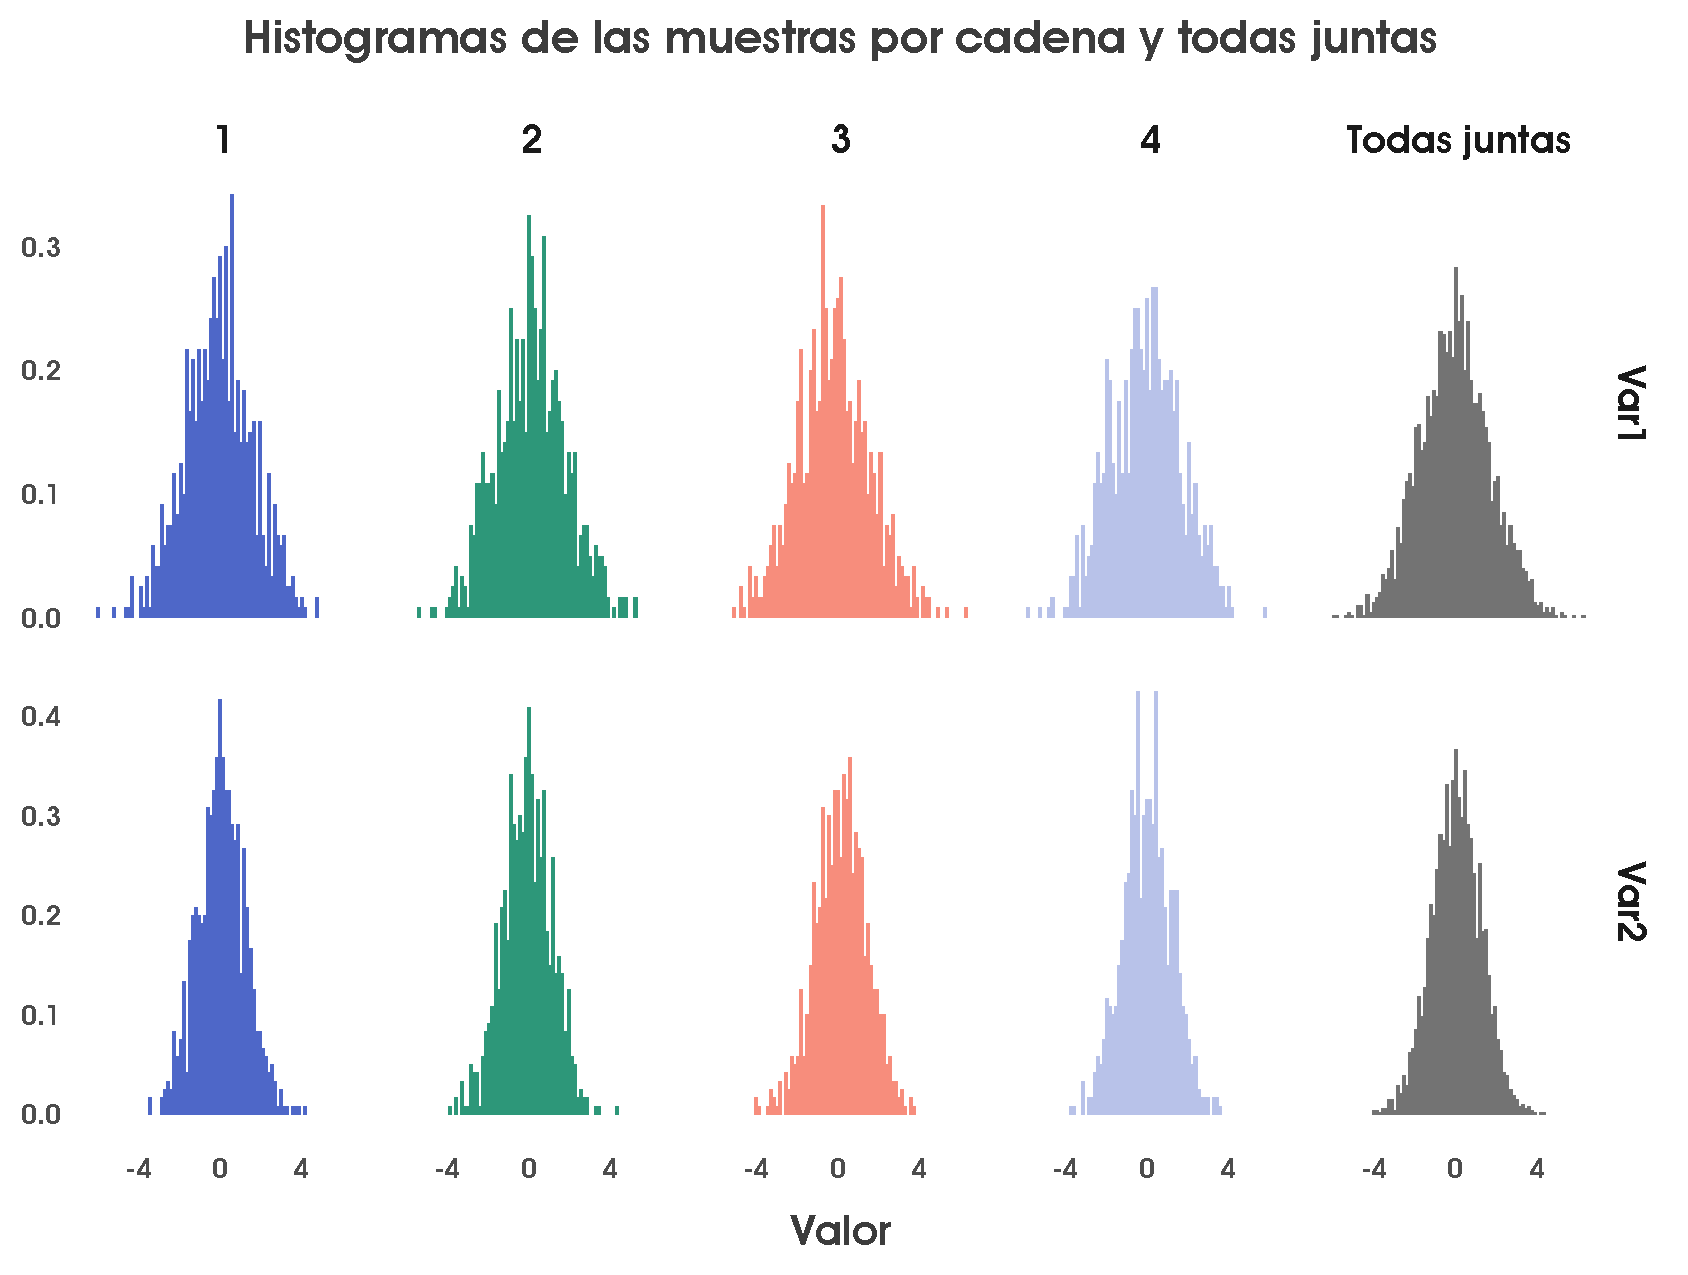
\includegraphics[width=0.9\textwidth]{Figs/Bayes/Ejemplos_Convergencia_Histogramas}
	\caption{Comparación de histogramas para las 4 cadenas de \textit{Gibbs Sampling} considerando solo las iteraciones válidas. Fuente: elaboración propia.}
	\label{fig:Conv_Hist}	
\end{figure}

A pesar de su utilidad, siempre hay que tener presente que los diagnósticos gráficos pueden ser engañosos y no bastan por si solos. Si la distribución es multimodal, por ejemplo, los gráficos de oruga pueden no mezclarse porque cada cadena explora una moda distinta.\\ 

Por otro lado, existen también resúmenes estadísticos para evaluar convergencia. Una estadística frecuentemente utilizada y que es normalmente reportada en softwares de cómputo mediante MCMC es el \textit{factor de reducción de escala} $\hat{R}$ propuesto por \textcite{GelmanRubin92}. Este está basado en comparar las varianzas de los parámetros o resúmenes inferenciales a través de las cadenas con aquellos dentro de cada cadena. La $\hat{R}$, bajo supuestos de normalidad, tiende a 1 conforme la convergencia aumenta. Por ello, un valor empírico cercano a 1, es normalmente requerido antes de poder declarar la convergencia.\\

Finalmente, querría comentar que hay 3 factores principales que permiten tener un buen muestreador de MCMC \parencite{Neal93}. El primero es la cantidad de cómputo requerida para simular cada transición; esta, por ejemplo, podría ser una ventaja de \textit{Gibbs Sampling} sobre \textit{Random Walk Metropolis} pues al aceptar todas las propuestas nos ahorramos la necesidad de realizar la corrección de Metropolis. El segundo factor es el tiempo que le lleva a la cadena alcanzar la convergencia; esto indica de manera general la cantidad de cómputo invertido en el periodo de calentamiento que se descartará. El tercer y útlimo factor está relacionado con el segundo pero es ligeramente diferente: las transiciones necesarias para movernos de un estado en la distribución objetivo a otro prácticamente independiente. Esto nos indicará el tamaño de la simulación requerido para realizar una estimación con alguna precisión deseada. Es normalmente este tercer factor el que motiva el uso de un muestreador distinto a RWM o a \textit{Gibbs Sampler} y que introduzco a continuación.\label{factor_ventaja_HMC}

\section{Hamiltonian Monte Carlo}

Una distribución posterior puede ser vista como una superficie de cimas y valles. Por ejemplo, la distribución normal--- identificada por su típica forma de campana--- sería una cima central. Imaginemos que queremos tener una muestra aleatoria de esta distribución. Esperaríamos tener más muestra en la región central--- al rededor de la moda--- que en las colas de la distribución, como puede verse en la \textbf{Figura \ref{fig:Muestra_Normal_Original}}. Si volteamos la función de densidad--- tomando el menos logaritmo, por ejemplo--- esta se convierte en una especie de tazón. Las regiones cercanas a la moda ahora son zonas bajas y las colas son zonas altas. La muestra se concentra en el fondo del tazón y no en los bordes, como puede verse en la \textbf{Figura \ref{fig:Muestra_Normal_Volteada}}.\\

\begin{figure}[h]
	\centering	
	\begin{subfigure}{0.45\textwidth}
        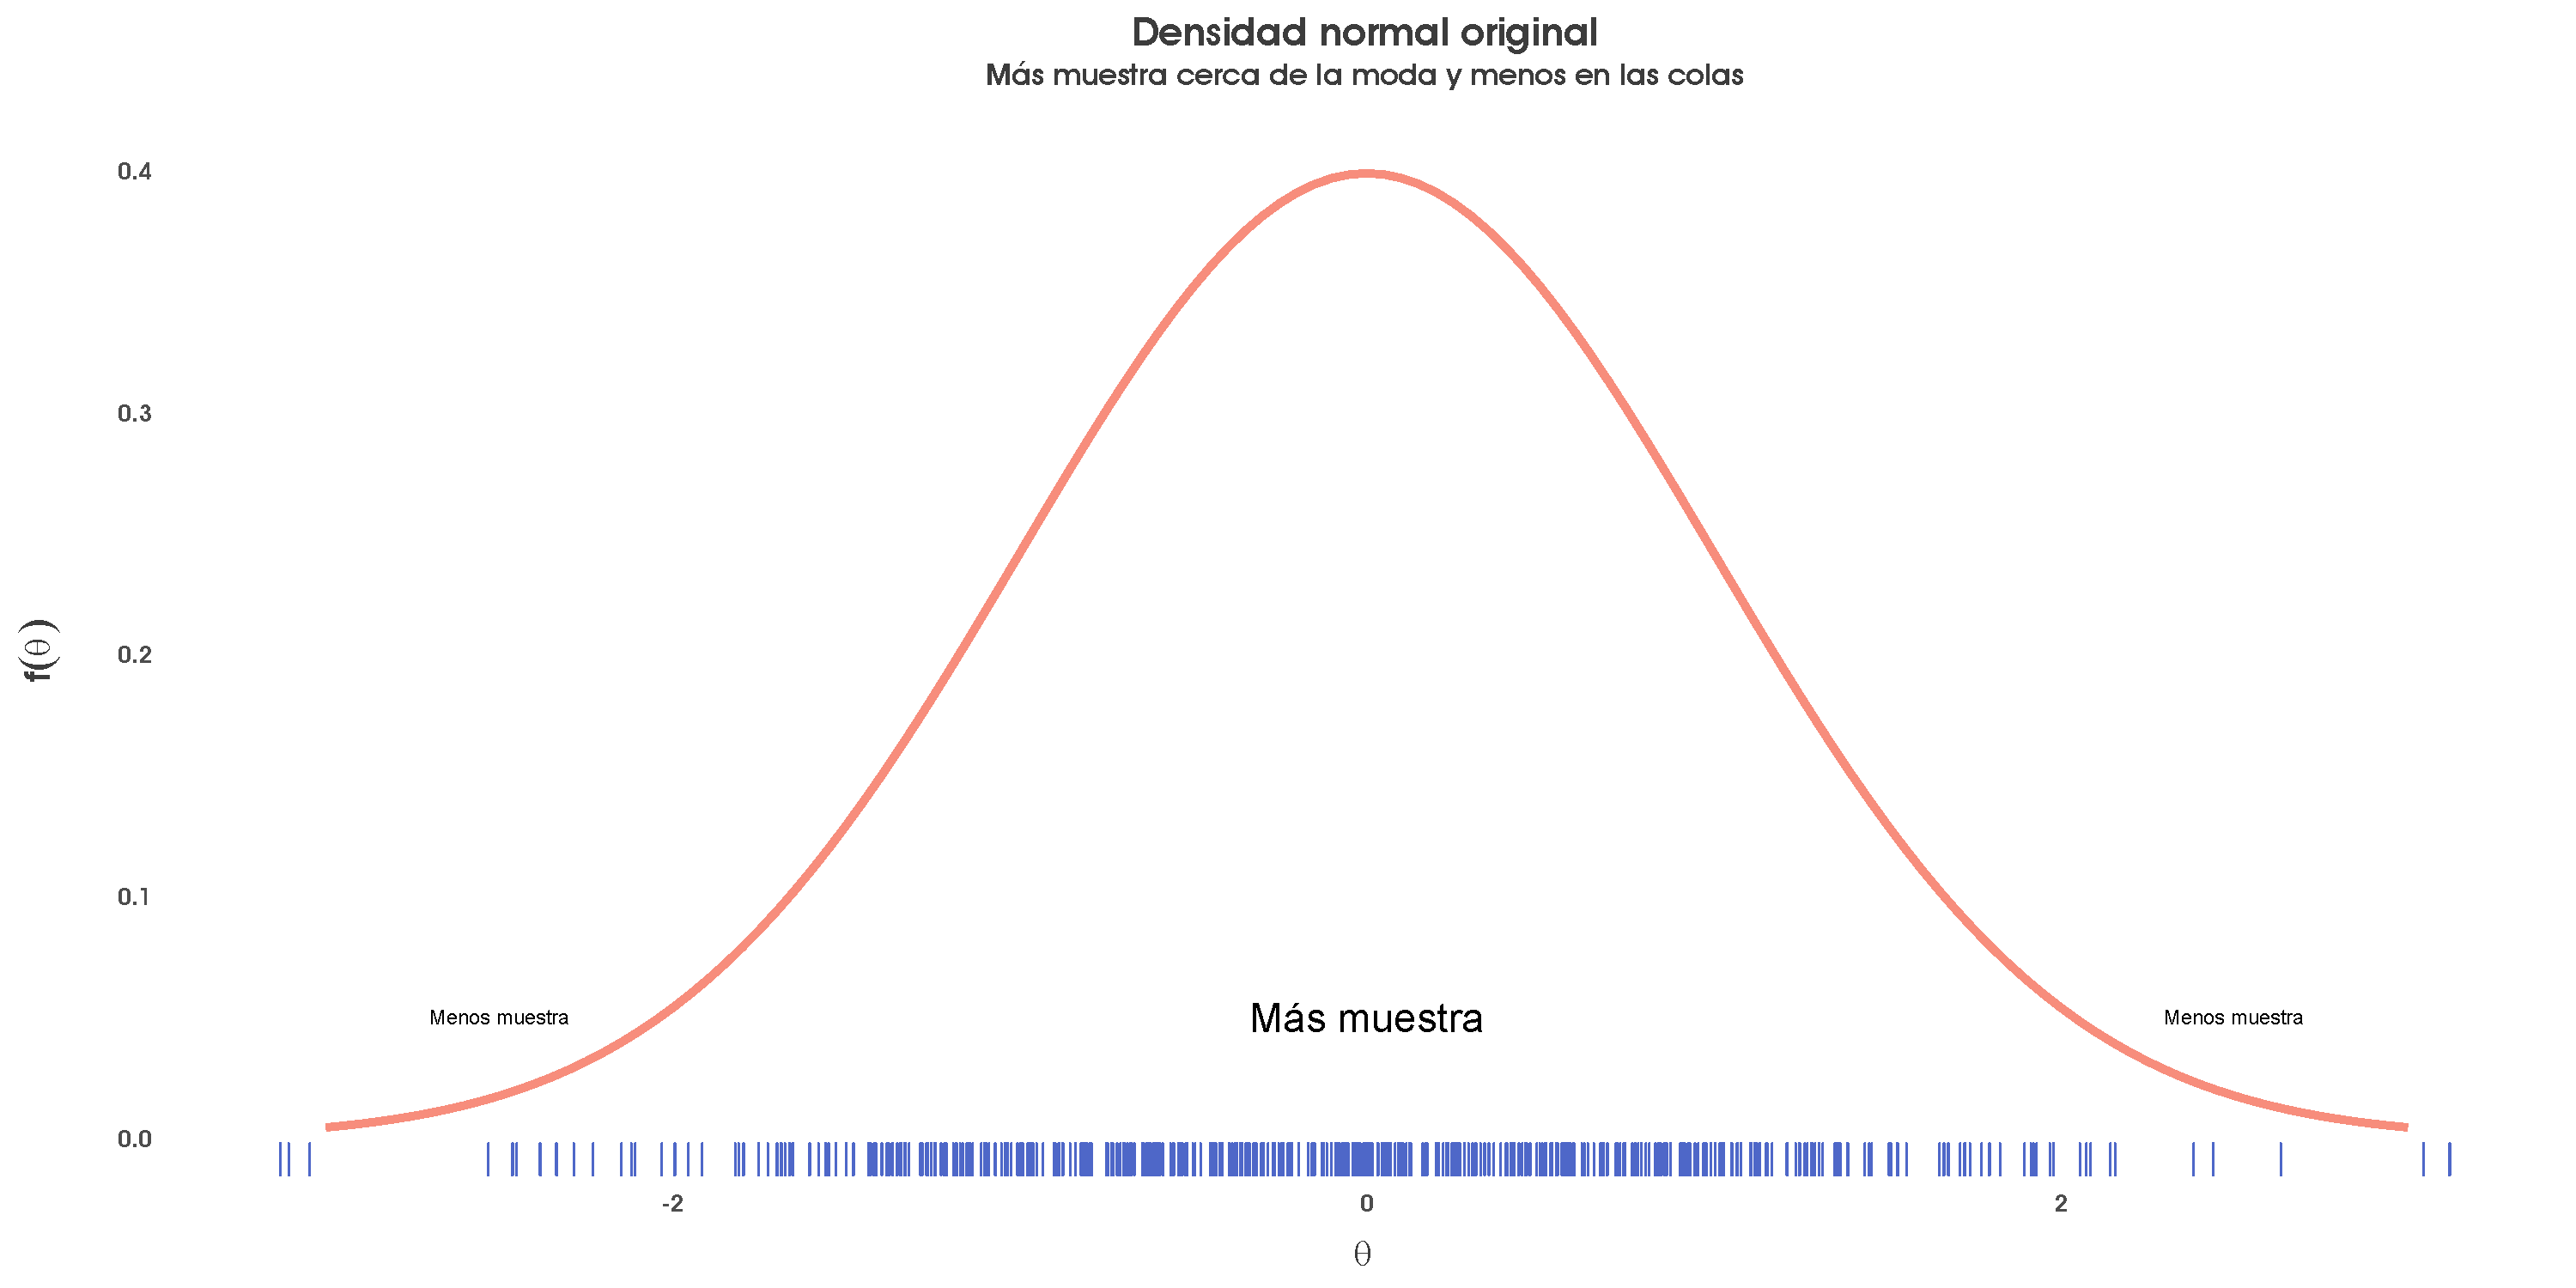
\includegraphics[width=\textwidth]{Figs/Bayes/Muestra_Normal_Original}
        \caption{La densidad original puede verse como una superficie con una cumbre al rededor de la cual se concentra la mayoría de las observaciones provenientes de una muestra aleatoria.}
        \label{fig:Muestra_Normal_Original}
    \end{subfigure}
    ~ 
    \begin{subfigure}{0.45\textwidth}
        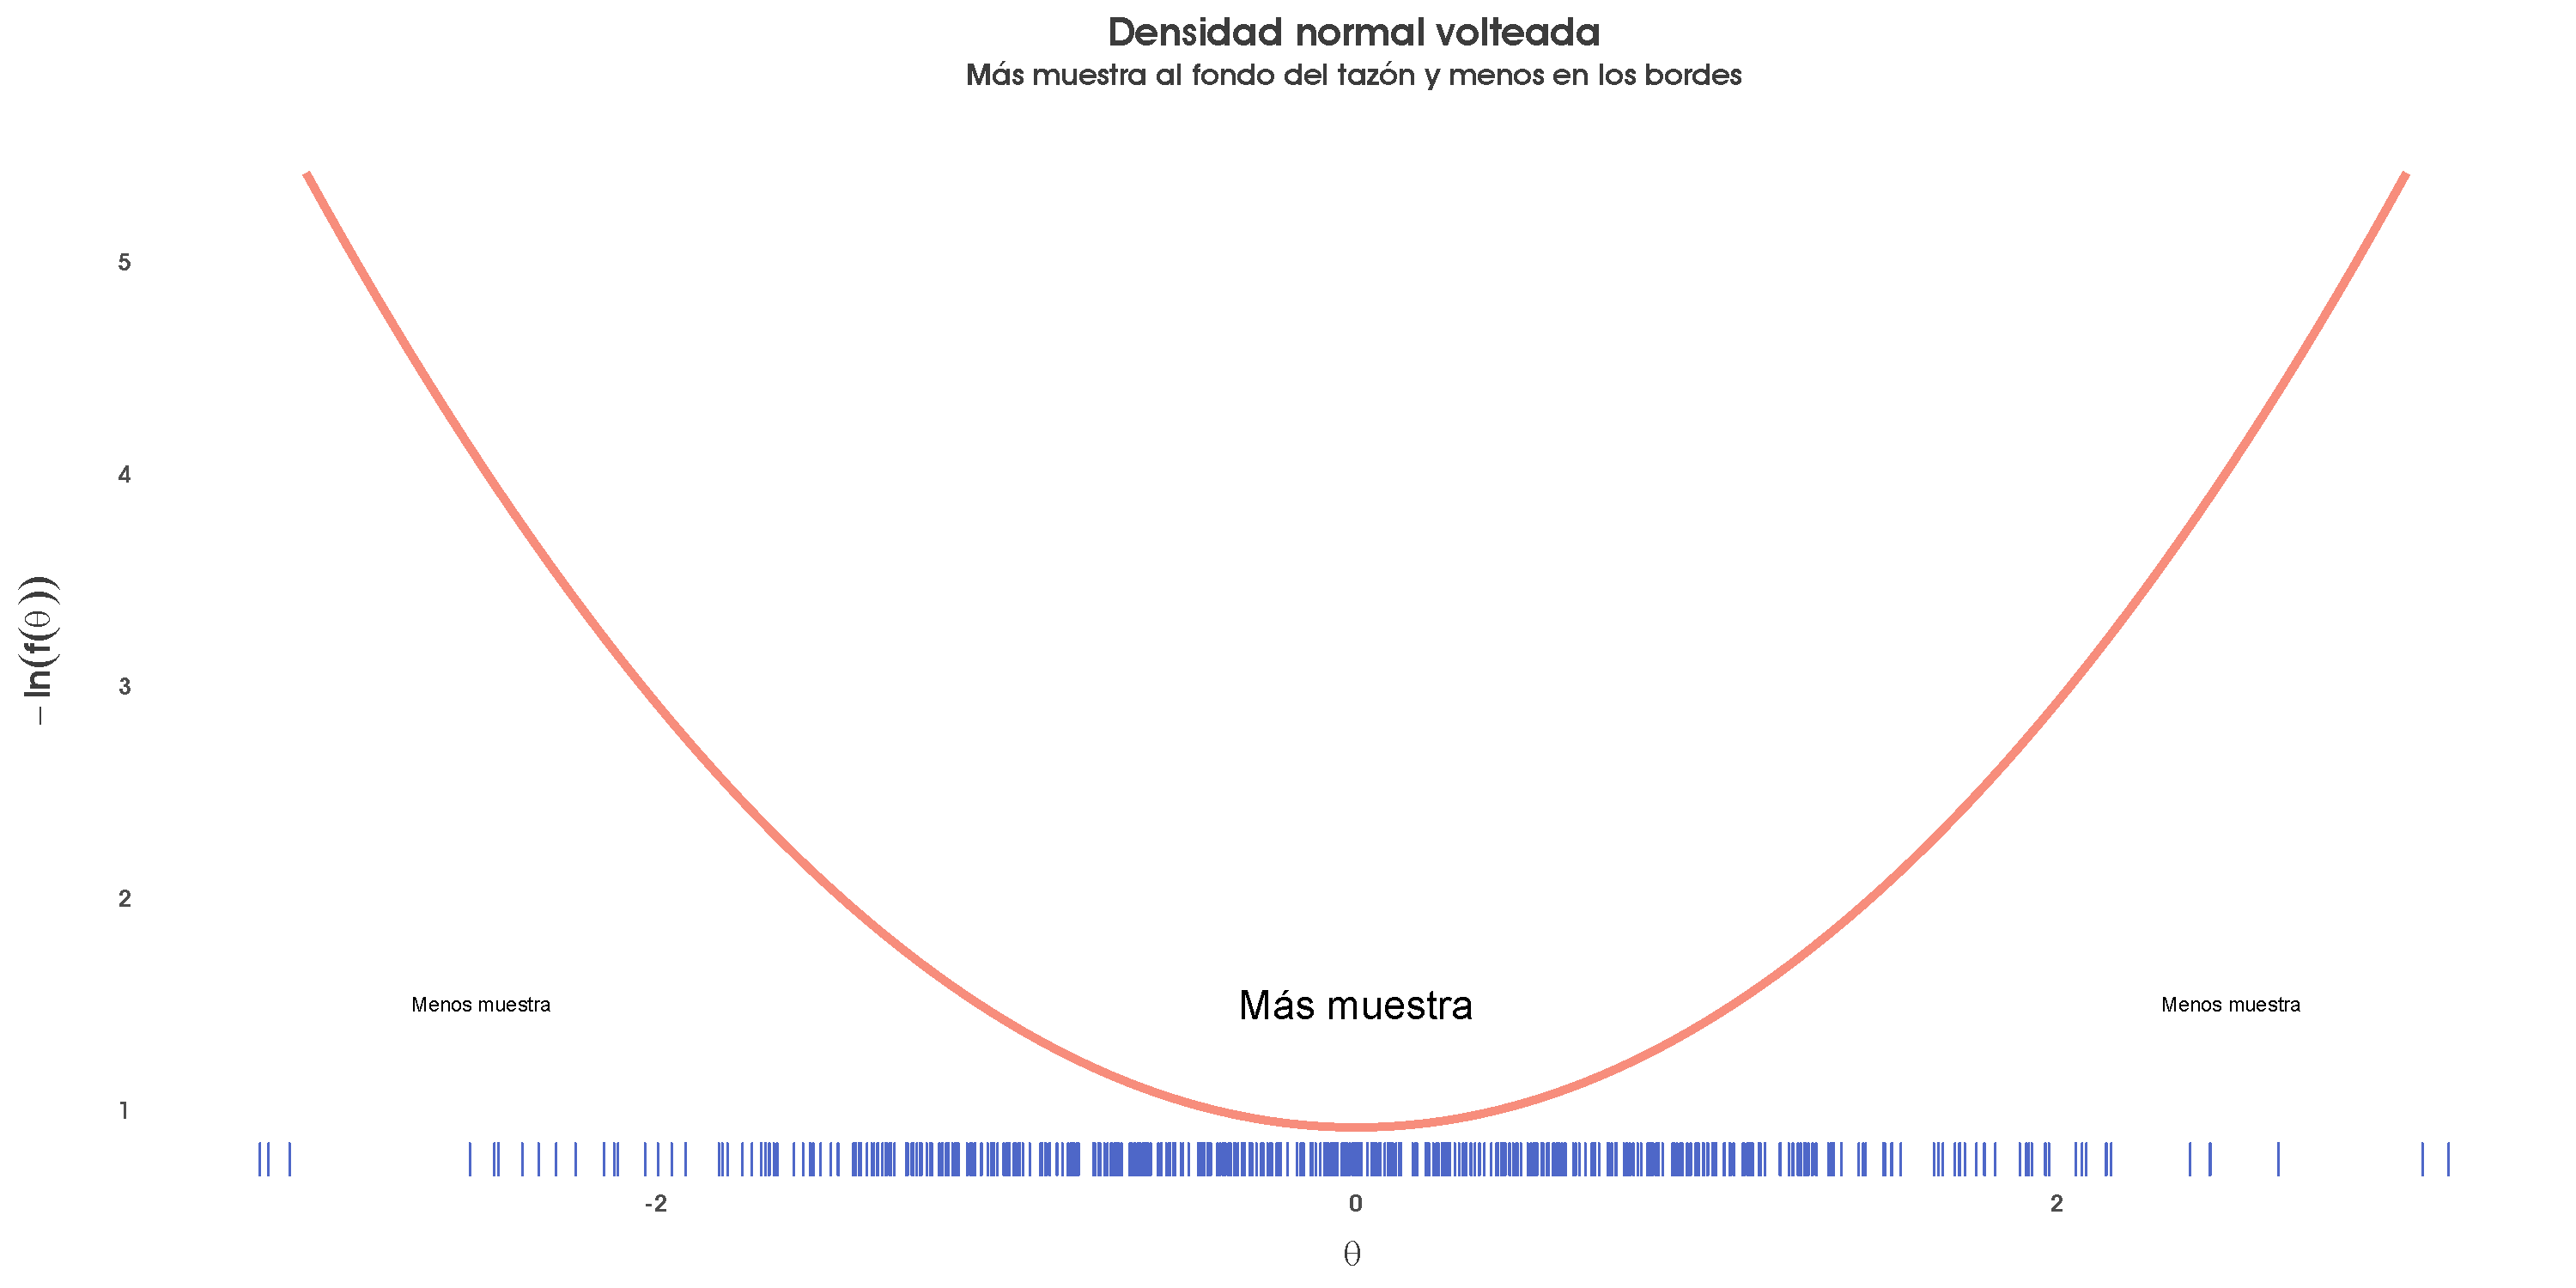
\includegraphics[width=\textwidth]{Figs/Bayes/Muestra_Normal_Volteada}
        \caption{Si volteamos y suavizamos la densidad aplicando el menos logaritmo, vemos que ahora la gráfica parece un tazón. La muestra se concentra en el fondo del tazón, en lugar de en los bordes del mismo.}
        \label{fig:Muestra_Normal_Volteada}
    \end{subfigure}
	\caption{Una muestra aleatoria proveniente de una distribución tiende a concentrarse al rededor de las modas. En los gráficos, las observaciones de una muestra aleatoria particular proveniente de la distribución normal se muestran mediante un \textit{rug plot} como marcas azules en el eje horizontal. Fuente: elaboración propia con base en la explicación de \textcite{Lambert18}.}
	\label{fig:Muestra_Normal}	
\end{figure}

 Imaginemos una partícula en algún punto de la superficie del tazón. Si le aplicáramos una cantidad de movimiento o \textit{momentum}, esta rodaría hacia el fondo del mismo, siguiendo las leyes de la física, como ilustro en la \textbf{Figura \ref{fig:Part_Rodando_A}}}. Si asumimos que no existe fricción, la partícula continuaría subiendo y bajando, intercambiando energía cinética por energía potencial y viceversa (\textbf{Figura \ref{fig:Part_Rodando_B}}).\\ 
 
\begin{figure}[h]
	\centering	
	\begin{subfigure}{0.45\textwidth}
        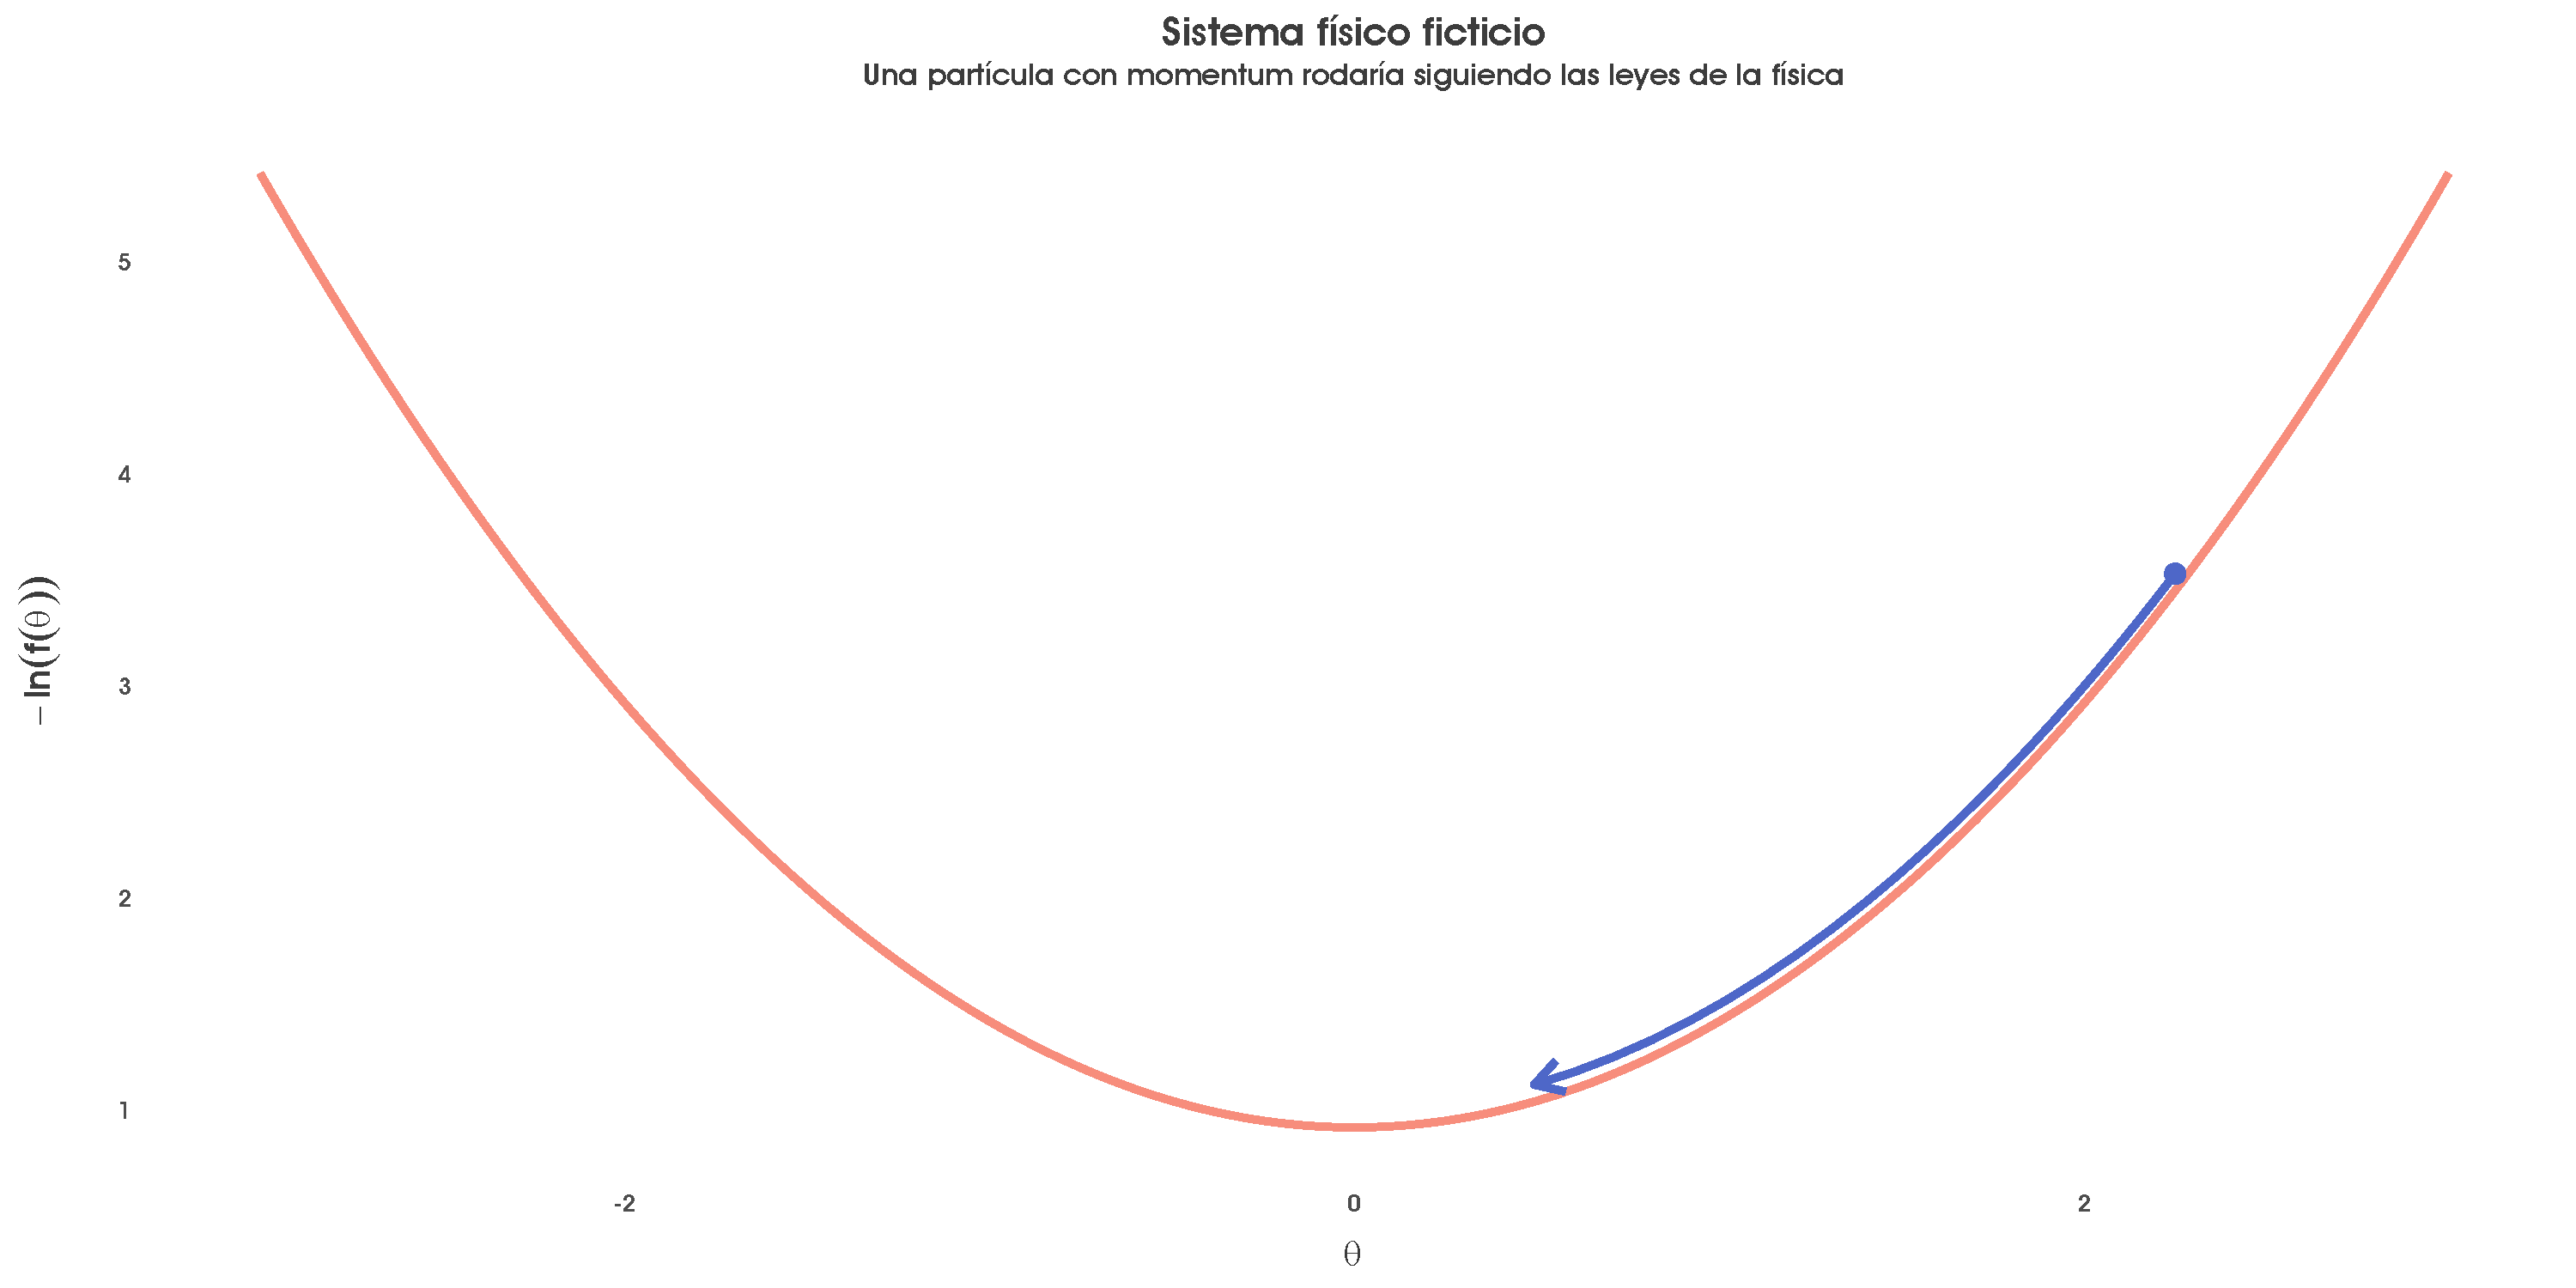
\includegraphics[width=\textwidth]{Figs/Bayes/Part_Rodando_A}
        \caption{Si una partícula en algún punto del tazón es puesta en movimiento, esta seguiría las leyes de la física y rodaría hacia el fondo del tazón.}
        \label{fig:Part_Rodando_A}
    \end{subfigure}
    ~ 
    \begin{subfigure}{0.45\textwidth}
        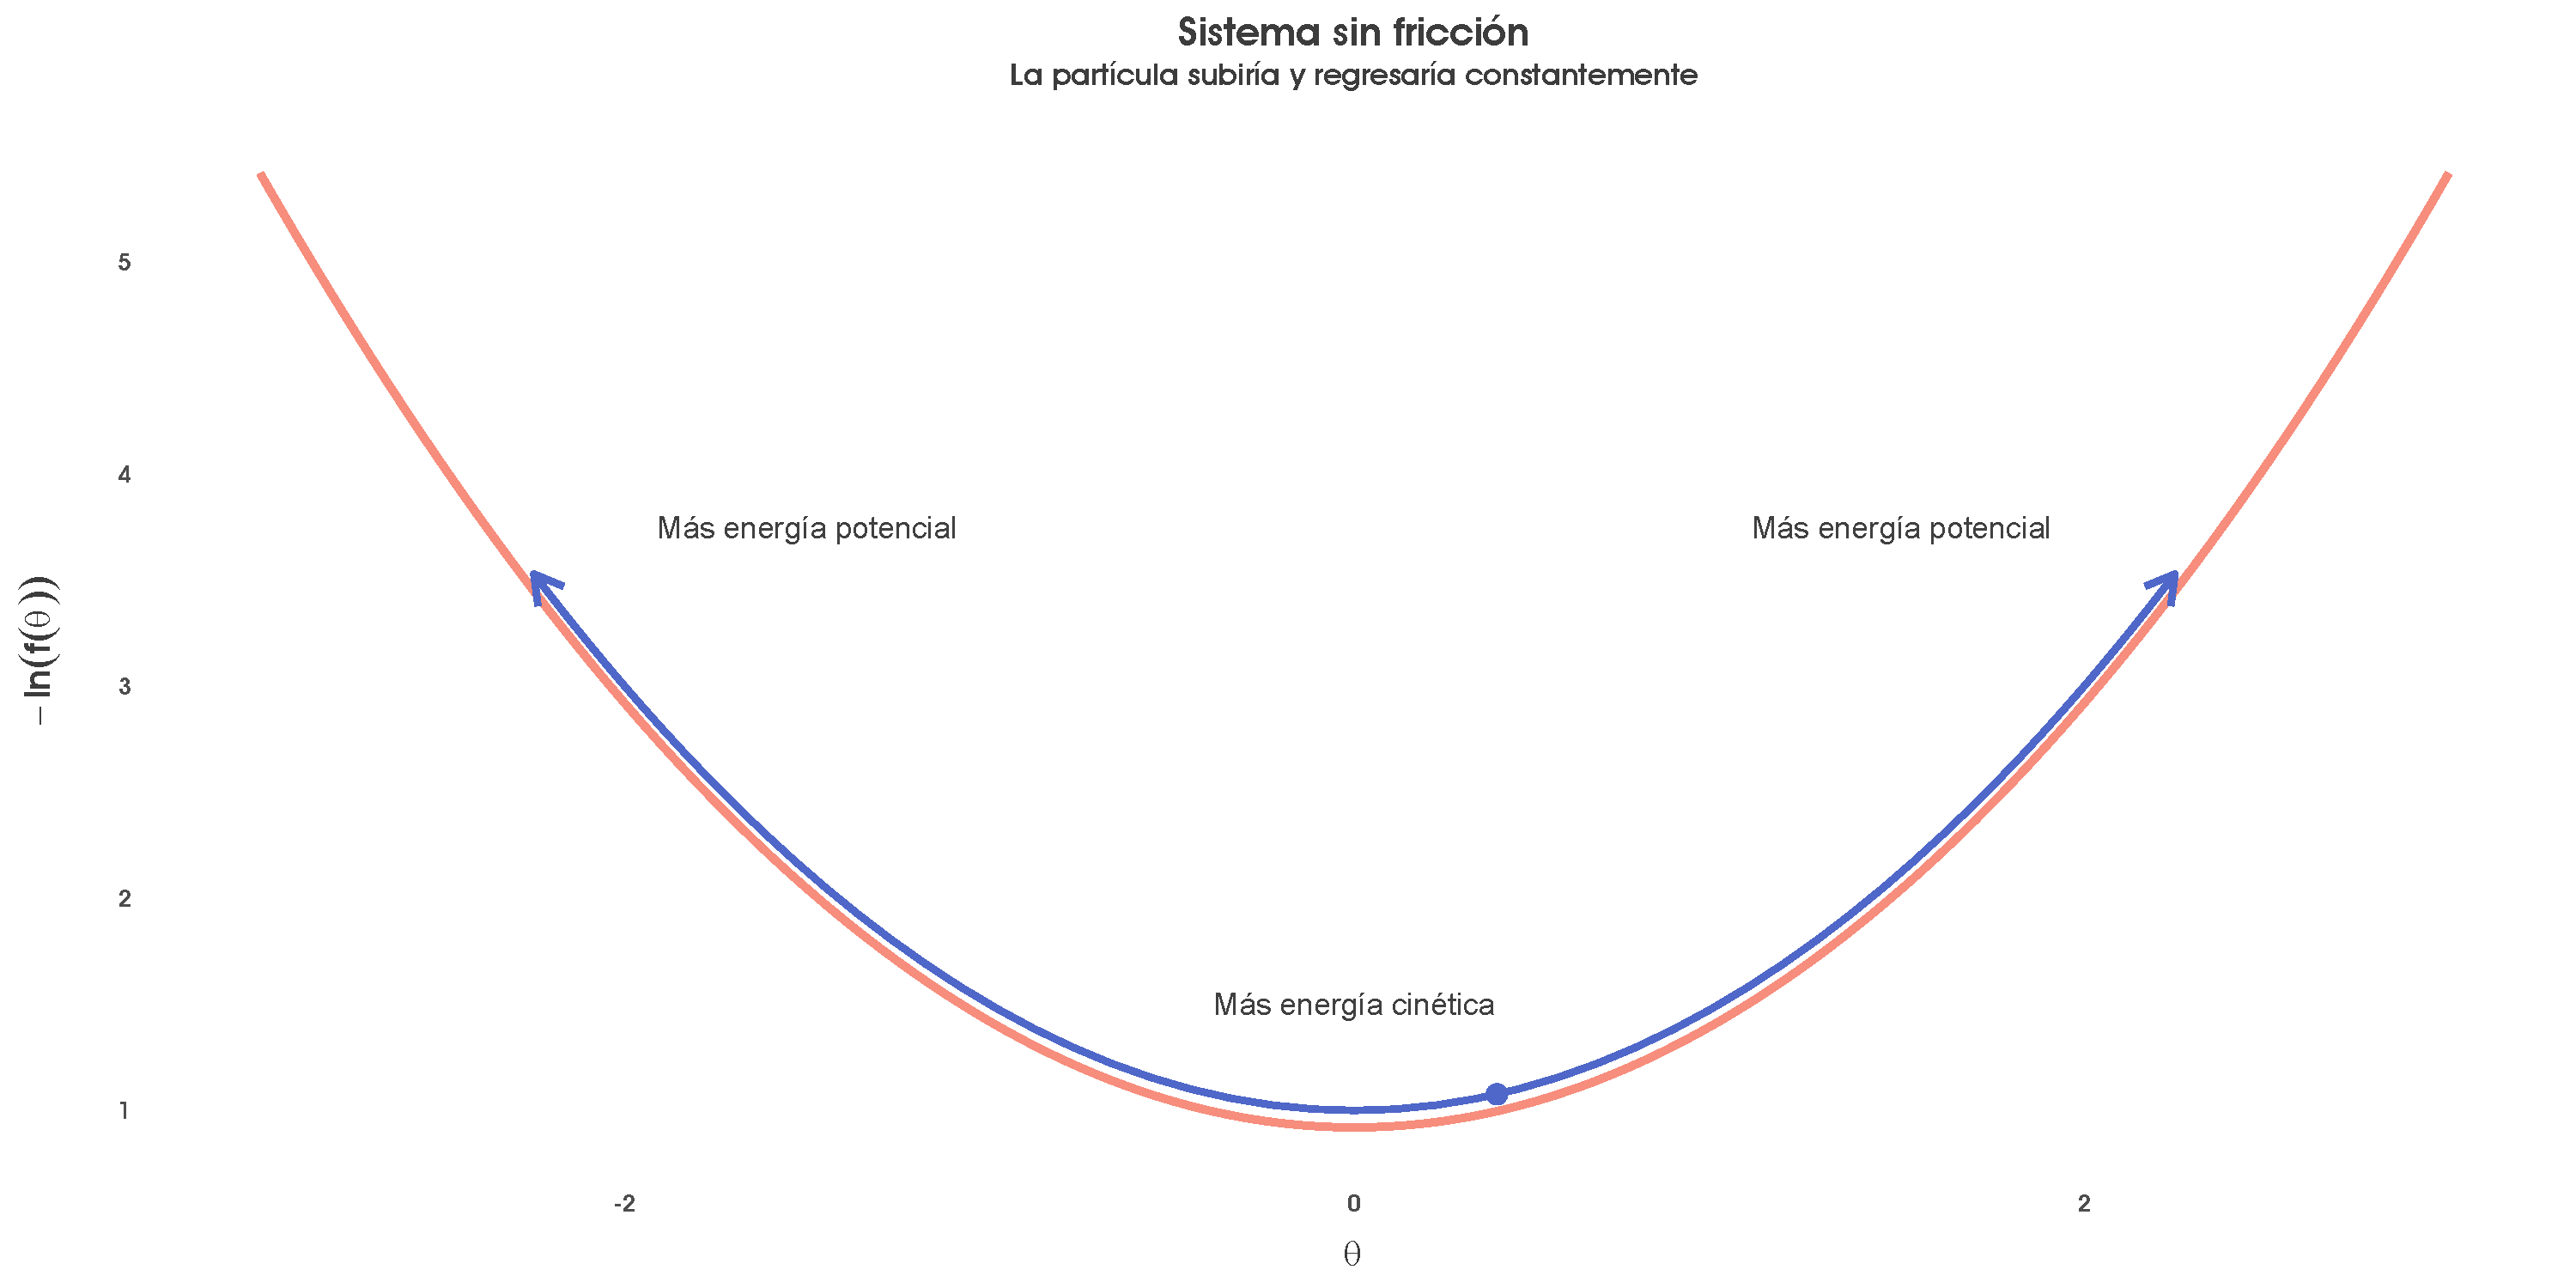
\includegraphics[width=\textwidth]{Figs/Bayes/Part_Rodando_B}
        \caption{Si suponemos que no hay fricción, la partícula recorrería continuamente una trayectoria en la que intercambiaría energía potencial y cinética, mientras sube y baja sobre la superficie, pasando por el fondo del tazón.}
        \label{fig:Part_Rodando_B}
    \end{subfigure}
	\caption{Para una densidad, podemos construir un sistema físico ficticio en el que partículas imaginarias recorrerían trayectorias sobre la superficie de la densidad volteada. Fuente: elaboración propia con base en la explicación de \textcite{Lambert18}.}
	\label{fig:Part_Rodando}	
\end{figure}
 
 Si tomamos otra partícula con otro \textit{momentum}, esta tendría una trayectoria distinta pero que también recorrería la superficie del tazón. Bajo esta dinámica, podemos conjeturar que una partícula tendería a estar más cerca del fondo del tazón que de los bordes, justo como una observación muestreada de la distribución que diera origen al tazón.\\ 
 
 Lo maravilloso de esta idea es que puede ser utilizada para obtener realizaciones provenientes de una distribución objetivo y realizar estimaciones de Monte Carlo. Es decir, podemos simular este sistema físico imaginario para construir una cadena de Markov y obtener una muestra de MCMC que no solo cumpla la intuición de tener más observaciones cerca de las modas que en las colas, sino que lo haga en la proporción correcta que marca la ley de probabilidad objetivo. Más aún, no requerimos conocerla \textit{por completo}, pues ``una pelota no conoce la superficie sobre la que rueda, sin embargo su camino está gobernado por ella'' \parencite{McElreath17}. Nos basta conocer la densidad objetivo salvo por una constante de normalización.\\ 
 
 De manera informal, lo único que debemos hacer es imaginar una partícula y ``empujarla'' en alguna dirección. Luego seguimos por un tiempo la trayectoria que las leyes de la física determinarían sobre la superficie de nuestra densidad volteada y la ``detenemos''. En este punto registramos su posición en el eje horizontal como una realización de nuestra variable aleatoria. Si volvemos a empujarla en otra dirección aleatoria y la seguimos por otro periodo de tiempo llegaríamos a una nueva posición que sería nuestra siguiente observación. Repitiendo este procedimiento obtendríamos una secuencia de observaciones que consituirían nuestra cadena de Markov.\\ 
 
 Este método de MCMC se conoce como \textit{Hamiltonian Monte Carlo} o HMC y procederé a exponerlo a continuación. Pero para entenderlo mejor, primero hay que introducir un poco de terminología del campo de la física estadística, para lo que seguiré la explicación de \textcite{Neal93}.\\
 
\subsection{Sistemas físicos} 
 
 Imaginemos que tuviéramos una descripción microscópica completa de un sistema físico. Por ejemplo, que conociéramos la posición y velocidad de todas las partículas de un sistema en un momento dado en el tiempo. Esta descripción se conoce como el \textit{microestado} del sistema. Evidentemente, en la realidad no podemos observar dicho microestado; más bien observamos el \textit{macroestado} del sistema, que incluye la temperatura o el volumen. Por ello, debemos asignar una medida de probabilidad sobre los microestados que podrían llevar al macroestado que observamos.\\ 
 
 Por ejemplo, supongamos que tenemos un sistema que mantiene una temperatura constante $T$ pero en el que cada microestado $s$ tiene una cierta energía $H(s)$.\footnote{En física, y en la referencia de \textcite{Neal93}, se utiliza la notación $E(s)$, pero para evitar confuciones con el valor esperado de $s$ y para facilitar la explicación de Hamiltonian Monte Carlo, utilizo la letra $H$. Asimismo, utilizaré otras notaciones no comunes en física, con la intención de ser más adecuadas al contexto estadístico.} Normalmente se supone que se satisface la siguiente \textit{distribución canónica}, también conocida como de Gibbs o de Boltzmann: 
 
\begin{equation}
\label{eq:Gibbs_Distr_Can}
 f(s) = \dfrac{exp\left\lbrace-H(s)/T\right\rbrace}{Z},
\end{equation}
 
 donde $Z$ es la constante de normalización y $H(s)$ es la función de energía del sistema y que depende del microestado en el que este se encuentre.\\
 
 Esta distribución canónica es particularmente útil porque \textit{cualquier} distribución de probabilidad que no valga cero en ningún punto puede ser expresada de esta manera. Para ver por qué, consideremos que tenemos un vector de variables aleatorias $s$, cuya distribución de probabilidad es $f(s)$. Esta puede considerarse una distribución canónica como \eqref{eq:Gibbs_Distr_Can} si consideramos que $s$ representa los microestados de un sistema físico ficticio con temperatura $T$ y constante de normalización $Z$ cuya función de energía esté dada por $H(s) = -T\,ln\left[Z\,f(s)\right]$. Por construcción, podríamos decir que la temperatura constante es $T=1$ y eliminarla de las ecuaciones.\\ 
 
 Esto quiere decir que podemos interpretar a una variable aleatoria como microestado de un sistema físico imaginario con distribución canónica para alguna función de energía conveniente. En particular, regresemos al caso en que queremos muestrear de la distribución posterior $f(\theta|y)$ de nuestro vector de parámetros de interés $\theta = (\theta_1,\dots,\theta_d)$. Diremos que los parámetros representan las coordenadas de la \textit{posición} de una partícula en un sistema físico y la expresamos como una distribución canónica con \textit{energía potencial} $U(\theta|y) = -ln\left[f(y|\theta)f(\theta)\right]$: 
\begin{equation*}
 f(\theta|y)=\dfrac{f(y|\theta)f(\theta)}{f(y)}=\dfrac{exp\left\lbrace -U(\theta|y)\right\rbrace}{Z_y},
\end{equation*} 
con $Z_y = f(y)$. Esta energía potencial es, precisamente, la forma de ``voltear'' la densidad que mencionaba al inicio de la sección.\\
 
 Por construcción, introduzcamos un vector adicional $m = (m_1,\dots,m_d)$, con una variable $m_i$ para cada uno de los $d$ parámetros $\theta_i$, que represente la cantidad de movimiento o \textit{momentum} de esta partícula ficticia. Este vector también tiene una distribución de probabildad $f(m)$ que usualmente es independiente de $\theta$ y de los datos. En este caso, tendríamos una \textit{energía cinética} $K(m)$ para la representación en distribución canónica: 
 \begin{equation*}
f(m)=\dfrac{exp\left\lbrace -K(m)\right\rbrace}{Z_m}
 \end{equation*} 
 Usualmente, por conveniencia y eficacia esta distribución será una normal centrada en cero pero cabe aclarar que $f(m)$ no \textit{necesita} ni ser independiente, ni ser gaussiana \parencite{Betancourt17}.\\
 
 Así pues, tenemos un espacio ampliado $2d$-dimencional y una distribución conjunta $f(\theta,m|y)=f(\theta|y)f(m)$. Dicho espacio para la posición y el \textit{momentum} de una partícula se conoce en física como \textit{espacio de fases}. De nueva cuenta, podemos construir la distribución canónica en este espacio; ahora, la función de energía total se llama el \textit{hamiltoniano} del sistema y es igual a la suma de las energías potencial y cinética, $H(\theta,m|y) = U(\theta|y) + K(m)$. En efecto, ignorando las constantes de normalización, 
 \begin{align*}
 f(\theta,m|y)&=f(\theta|y)f(m)\\
 &\propto exp\left\lbrace -U(\theta|y)\right\rbrace \, exp\left\lbrace -K(m)\right\rbrace\\
 &\propto exp\left\lbrace -\left[ U(\theta|y) + K(m)\right]\right\rbrace\\
 &\propto exp\left\lbrace -H(\theta,m|y)\right\rbrace.
 \end{align*}
 
 Notemos que si muestreamos de esta distribución canónica conjunta en el espacio de fases, automáticamente estaríamos muestreando de la distribución de nuestros parámetros $\theta$, pues solo debemos marginalizar ignorando los valores del vector auxiliar $m$. Para ello aprovecharemos que este sistema físico ficticio satisfaría las leyes de la mecánica hamiltoniana--- que es solo una reformulación de la mecánica clásica--- y utilizaremos una estrategia de dos pasos.\\ 
 
 En ausencia de fricción o injerencia externa, tendríamos que la energía total de una partícula--- i.e. el hamiltoniano que definimos como la suma de las dos energías--- se mantiene constante. Para ello, una partícula en movimiento debe ir convirtiendo energía potencial en energía cinética y viceversa. Recordemos la concepción de una densidad como una superficie de cimas y valles con una partícula deslizándose sobre ella, como ilustraba en la \textbf{Figura \ref{fig:Part_Rodando_B}}. La energía potencial de la partícula en cada instante es proporcional a la altura de la superficie en la posición en que se encuentre. Conforme se desliza hacia abajo, la energía potencial se va convirtiendo en energía cinética hasta llegar al fondo del tazón y empezar a deslizarse hacia arriba. Ahora la energía cinética es la que se va convirtiendo en energía potencial hasta llegar a un punto donde la partícula se detiene momentáneamente y comienza a deslizarse de regreso, repitiendo el proceso.\\ 
 
 La trayectoria que dicha partícula seguiría en el tiempo $\tau$ cumpliría las \textit{ecuaciones de Hamilton} \parencites{Neal93,Neal11,Betancourt17}: 
 \begin{equation}
 \label{eq:Ecuaciones_Hamilton}
 \dfrac{d\theta}{d\tau}=+\dfrac{\partial H}{\partial m} = \dfrac{\partial K}{\partial m} \qquad \text{y} \qquad \dfrac{d\,m}{d\tau}=-\dfrac{\partial H}{\partial \theta} = -\dfrac{\partial U}{\partial \theta}
 \end{equation}
 
 Estas ecuaciones diferenciales nos dicen cómo cambiarían $\theta$ y $m$ conforme avanza el tiempo en una simulación dinámica del sistema físico que construimos. Asimismo, podemos verificar que la energía se mantiene constante, viendo que el cambio del hamiltoniano en el tiempo es cero, sustituyendo \eqref{eq:Ecuaciones_Hamilton}:
 \begin{equation*}
 \dfrac{dH}{d\tau} = \sum\limits_{i=1}^d \dfrac{\partial H}{\partial \theta_i}\dfrac{d\theta_i}{d\tau} + \dfrac{\partial H}{\partial m_i}\dfrac{dm_i}{d\tau} = \sum\limits_{i=1}^d \dfrac{\partial H}{\partial \theta_i}\dfrac{\partial H}{\partial m_i} - \dfrac{\partial H}{\partial m_i}\dfrac{\partial H}{\partial \theta_i} = 0
 \end{equation*}
 
\subsection{HMC ideal y en la práctica} 
 
 La estrategia para muestrear de la distribución canónica en el espacio de fases es ir alternando pasos. Muestreamos primero de la distribución de $m$, dada una $\theta$ inicial; en el caso de independencia esta es simplemente la marginal de $m$. Luego, seguimos la trayectoria determinística que indican las ecuaciones de Hamilton.\\
 
 Para ilustrarlo, recordemos que en el ejemplo con el que empezaba la sección, el parámetro $\theta$ se distribuía como una normal estándar. Introduzcamos una variable independiente de \textit{momentum} $m$ también distribuida $N(0,1)$. En este caso, ambas energías son el menos logaritmo del kernel de una normal estándar, por lo que tendríamos que $U(\theta)=\dfrac{\theta^2}{2}$ y $K(m)=\dfrac{m^2}{2}$. Las ecuaciones de Hamilton \eqref{eq:Ecuaciones_Hamilton} resultan entonces ser
 \begin{equation*}
 \dfrac{d\theta}{d\tau}= \dfrac{dK}{dm} = m \qquad \text{y} \qquad \dfrac{d\,m}{d\tau}= -\dfrac{dU}{d\theta} = -\theta,
 \end{equation*}
 cuyas soluciones tienen una forma analítica conveniente, para algunas constantes $r$ y $a$ \parencite{Neal11}:
 \begin{equation}
 \label{eq:Trayectorias_Normal}
 \theta(\tau) = r\,cos(a + \tau) \qquad \text{y} \qquad m(\tau) = -r\,sen(a + \tau)
 \end{equation}
 
 La partícula de la \textbf{Figura \ref{fig:Part_Rodando}} en el espacio de fases se vería como en la \textbf{Figura \ref{fig:Primera_Trayectoria}}. La distribución canónica es una normal bivariada cuyas curvas de nivel determinan órbitas con energía/hamiltoniano constante a lo largo de las cuales se desplazarían las partículas ficticias sobre las trayectorias definidas por las ecuaciones de Hamilton.\\ 
 
 Si iniciamos con un valor de $\theta^{(0)}$, muestreamos un valor $m^{(0)} \sim f(m)$. Esto coloca a la partícula sobre una órbita particular con valor constante del hamiltoniano $H(\theta^{(0)},m^{(0)})$. Ahora seguimos por un tiempo $\tau$ la trayectoria definida por \eqref{eq:Trayectorias_Normal}. Esto nos lleva a una nueva coordenada $(\theta^{(1)},\tilde{m}^{(0)})$, desde la que registramos la posición $\theta^{(1)}$ como nuestra propuesta de observación muestreada. En este punto repetimos el procedimiento: generamos un nuevo valor $m^{(1)} \sim f(m)$, saltamos a una nueva órbita con hamiltoniano $H(\theta^{(1)},m^{(1)})$, seguimos la trayectoria por otro periodo $\tau$ para obtener $\theta^{(2)}$. En la \textbf{Figura \ref{fig:Primeras_Trayectorias}} se muestran 10 iteraciones de este procedimiento con los valores muestreados en los márgenes del gráfico como \textit{rug plot}.\\ 

\begin{figure}[h]
	\centering	
	\begin{subfigure}{0.4\textwidth}
        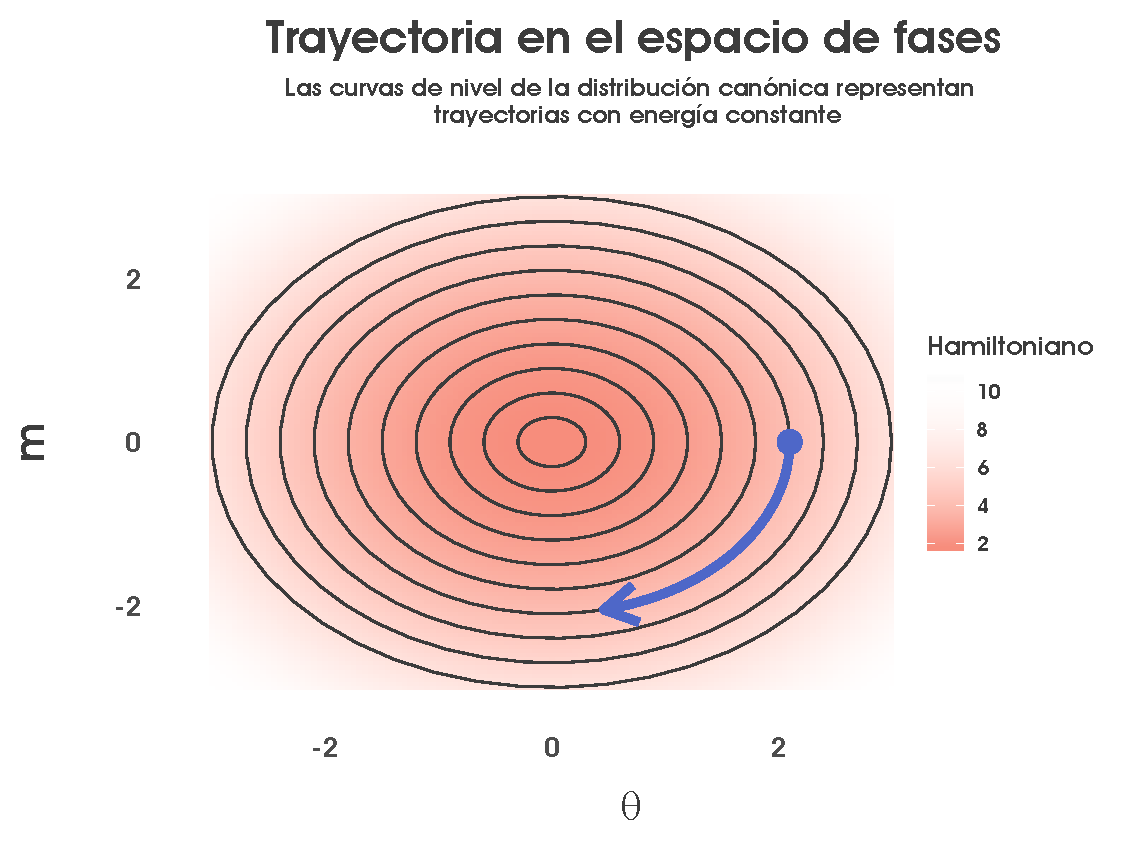
\includegraphics[width=\textwidth]{Figs/Bayes/Trayectoria_Espacio_Fase}
        \caption{Una partícula se mueve en el espacio de fase a lo largo de trayectorias definidas por las ecuaciones de Hamilton y que coinciden con las curvas de nivel de la distribución que mantienen el valor del hamiltoniano constante.}
        \label{fig:Primera_Trayectoria}
    \end{subfigure}
    ~ 
    \begin{subfigure}{0.4\textwidth}
        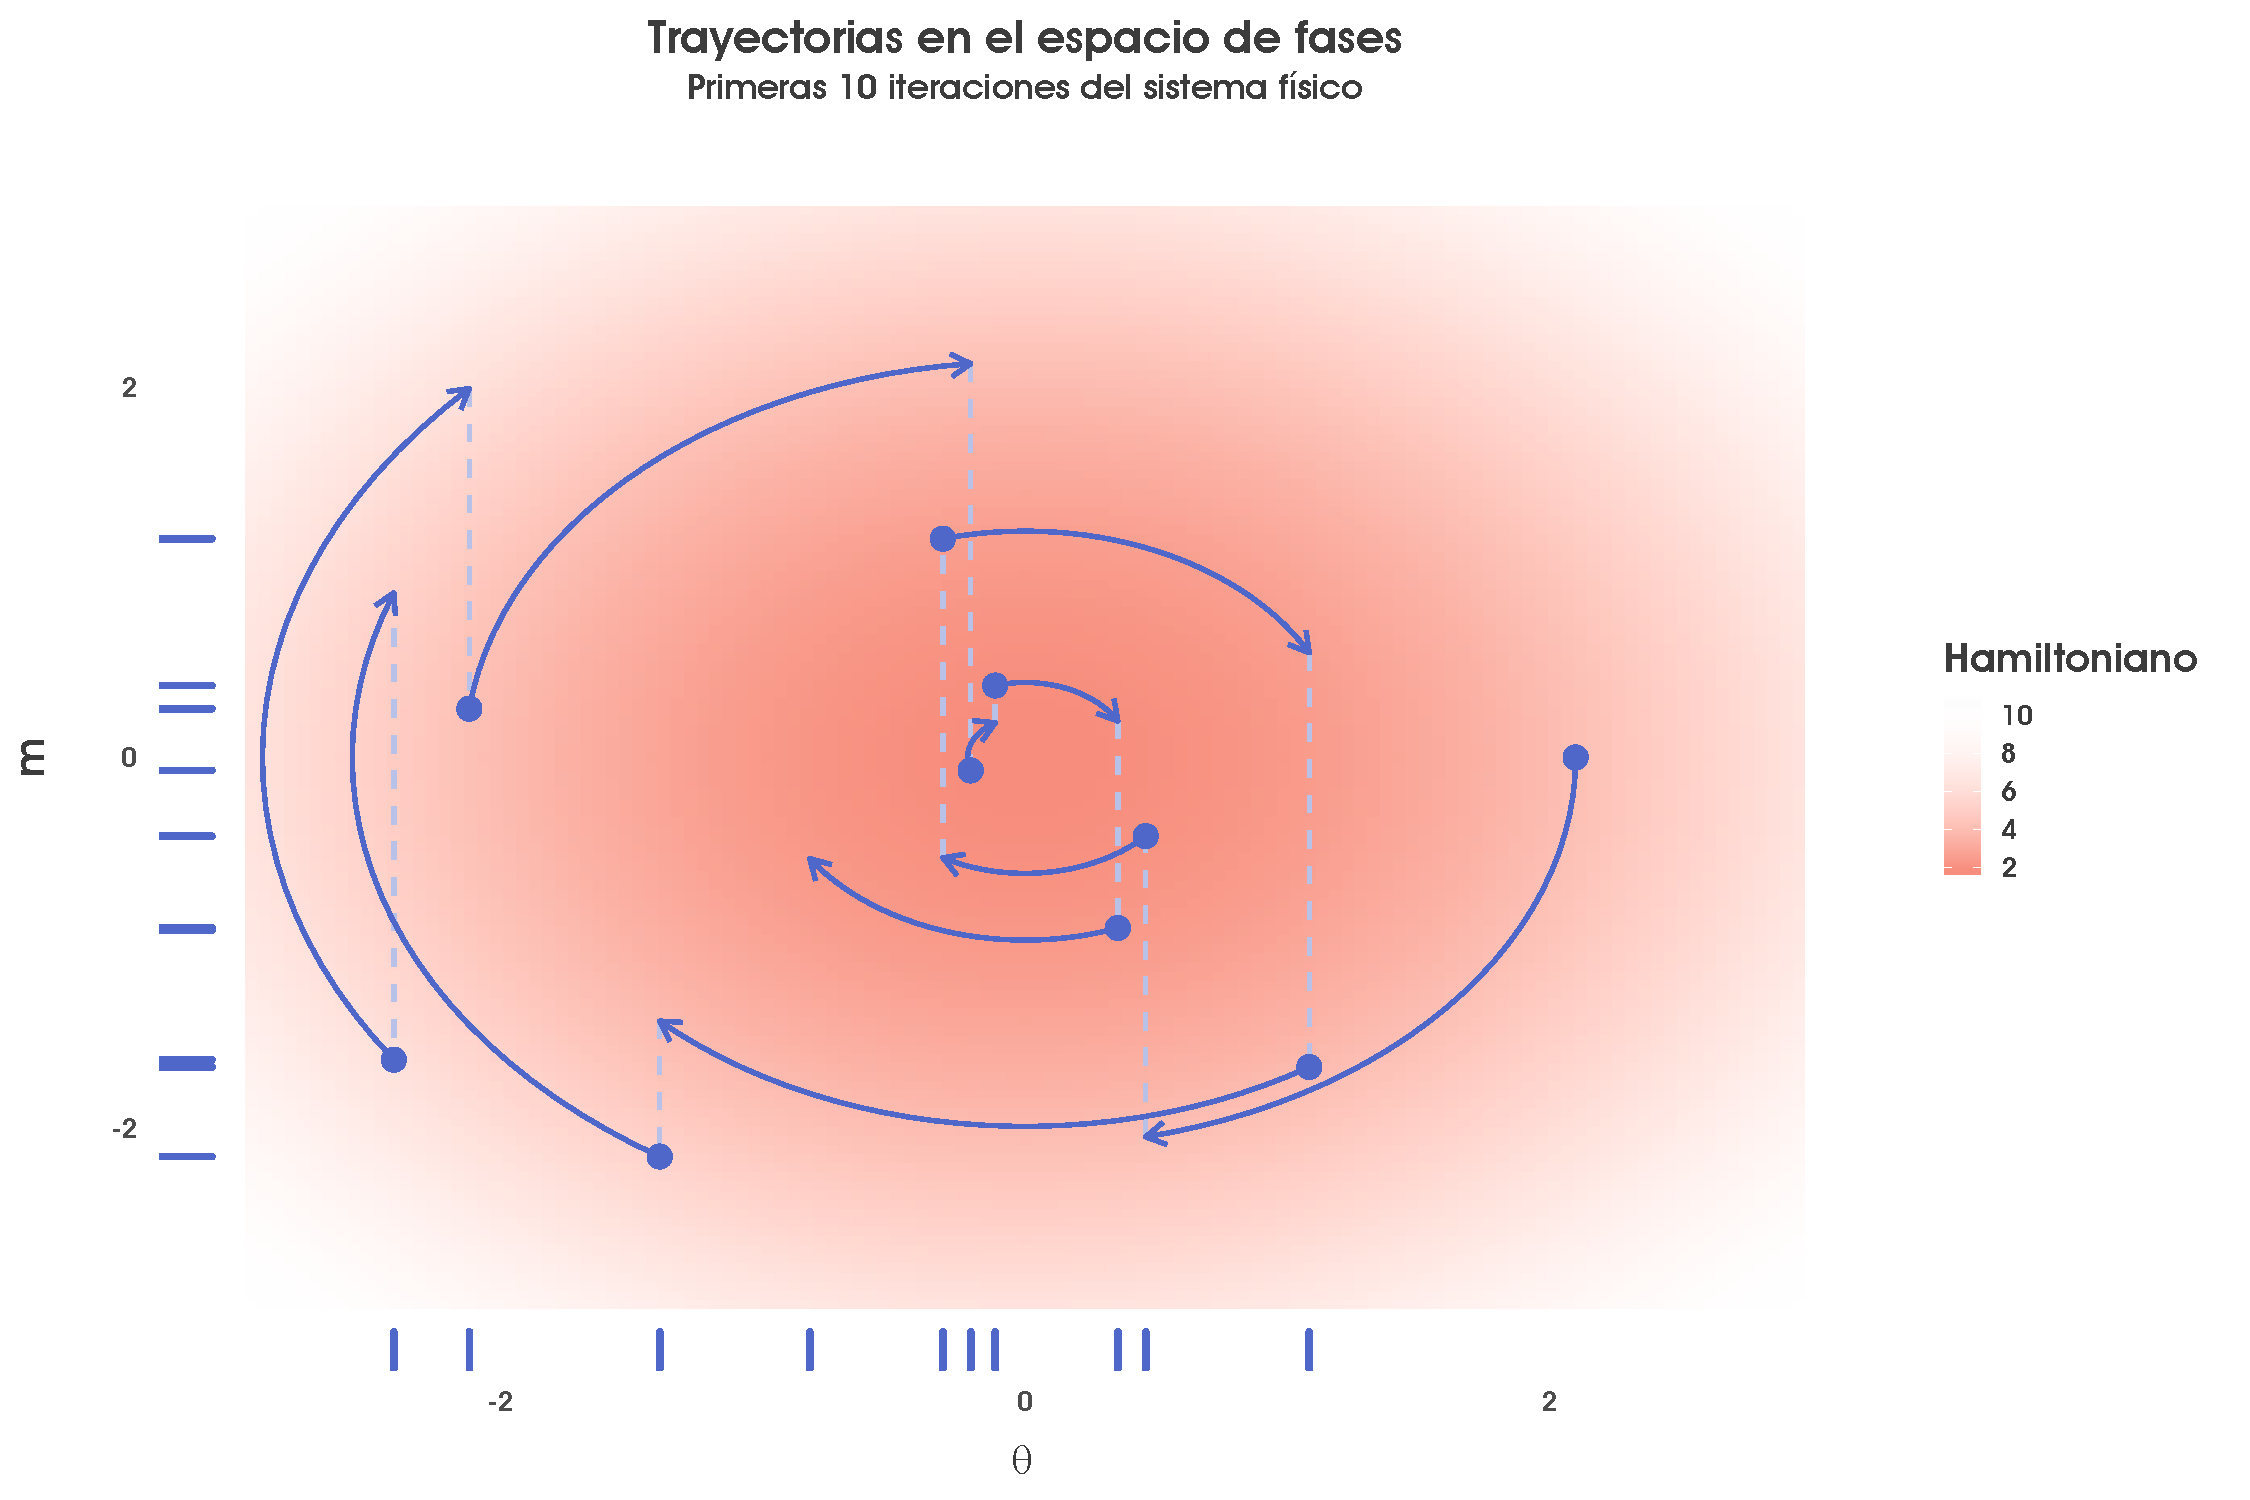
\includegraphics[width=\textwidth]{Figs/Bayes/Primeras_Trayectorias}
        \caption{Con una posición inicial $\theta^{(i)}$, se muestrea una cantidad de movimiento aleatoria $m^{(i)}$ (líneas punteadas). Esto lleva la partícula a una órbita específica. Después se sigue la trayectoria por un tiempo y se registra la nueva posición $\theta^{(i+1)}$ (flechas continuas). Se presentan las primeras 10 iteraciones de este procedimiento, con los valores muestreados como gráfico \textit{rug}.}
        \label{fig:Primeras_Trayectorias}
    \end{subfigure}
	\caption{Ilustración de las trayectorias definidas por la distribución canónica de un espacio de fases en el que tanto la posición como el \textit{momentum} se distribuyen normal estándar y en donde se muestrea mediante una estrategia de dos pasos. Fuente: elaboración propia con base en \textcite{Betancourt17}.}
	\label{fig:Trayectorias_Espacio_Fase}	
\end{figure}
 
Esta estrategia de dos pasos funcionaría como un algoritmo de \textit{Gibbs dentro de Metropolis-Hastings}. El primer paso--- muestrear un nuevo valor de \textit{momentum}--- constituye un paso de Gibbs pues, en general, estaríamos muestreando de la condicional de $m$ dada la $\theta$ anterior. Integrar las ecuaciones de Hamilton por un tiempo $\tau$, constituiría un paso de Metropolis-Hastings, respecto a la distribución canónica $f(\theta,m)$. Es decir, podemos pensar que seguir la trayectoria de la partícula por un tiempo $\tau$ constituye un kernel de propuestas $q(\tilde{\theta},\tilde{m}|\theta,m)$.\\ 

La única consideración téorica adicional es que, al finalizar de integrar la trayectoria por un tiempo $\tau$, se deberían negar las variables de \textit{momentum} para garantizar la reversibilidad de la cadena de Markov \parencite{Neal93,Neal11,Betancourt17}. Esta negación en la \textbf{Figura \ref{fig:Part_Rodando_A}} se vería simplemente como voltear la flecha. En las \textbf{Figuras \ref{fig:Trayectorias_Espacio_Fase}} la partícula saltaría al lado contrario de la misma órbita. Ahora bien, debemos notar que esta negación del \textit{momentum} vuelve al kernel de propuestas simétrico. Esta característica, junto con la propiedad de conservación del hamiltoniano--- pues no hemos cambiamos de órbita--- lleva a que siempre aceptemos las propuestas.\\ 

En efecto, si comenzamos en un punto $(\theta,m)$ y seguimos la trayectoria un tiempo $\tau$, llegamos a un nuevo punto $(\theta_\tau,m_\tau)$; negando el \textit{momentum} llegaríamos al punto $(\theta_\tau,-m_\tau)$ de manera determinista, por lo que  $q(\theta_\tau,-m_\tau|\theta,m) = 1$. Si ahora comenzamos en $(\theta_\tau,-m_\tau)$, la trayectoria ``regresaría sobre sus propios pasos'' excepto que con el signo contrario del \textit{momentum} hasta $(\theta,-m)$. Al completar la propuesta, negando de nueva cuenta el \textit{momentum}, regresaríamos exactamente a $(\theta,m)$. Así pues, resulta que también $q(\theta,m|\theta_\tau,-m_\tau) = 1$. Esto lleva a una probabilidad de aceptación \eqref{eq:Proba_Aceptar_MH} de 1:
\begin{align}
\alpha(\theta_\tau,-m_\tau;\theta,m) &= min\left\lbrace\dfrac{f(\theta_\tau,-m_\tau)q(\theta,m|\theta_\tau,-m_\tau)}{f(\theta,m)q(\theta_\tau,-m_\tau|\theta,m)},1\right\rbrace \nonumber \\
&= min\left\lbrace\dfrac{f(\theta_\tau,-m_\tau)}{f(\theta,m)},1\right\rbrace \nonumber\\
&= min\left\lbrace\dfrac{exp\left[ -H(\theta_\tau,-m_\tau)\right]}{exp\left[ -H(\theta,m)\right]},1\right\rbrace \nonumber\\
&= min\left\lbrace exp\left[ H(\theta,m)-H(\theta_\tau,-m_\tau)\right],1\right\rbrace, \nonumber\\
\intertext{y por conservación del hamiltoniano, $H(\theta,m)=H(\theta_\tau,-m_\tau)$, por lo que}
\alpha(\theta_\tau,-m_\tau;\theta,m)&= min\left\lbrace e^0,1\right\rbrace = 1.
\label{eq:Proba_Acepta_HMC_ideal}
\end{align}
Finalmente, como solo nos interesa conservar la nueva posición $\tilde{\theta}=\theta_\tau$ antes de muestrear un nuevo \textit{momentum}, la negación al final de la trayectoria no necesita llevarse a cabo \textit{en realidad}, por lo que el algoritmo puede proceder normalmente como los dos pasos antes mencionados.\\

Empero, todavía tenemos que considerar un detalle. Normalmente no tenemos tanta suerte como en el caso de la normal estándar y las ecuaciones de Hamilton no tienen una solución analítica simple. Esto quiere decir que tenemos que \textit{aproximar} las trayectorias. Afortunadamente existe una familia poderosa de métodos, conocidos como \textit{integradores simplécticos} que aproximan de buena manera. El lector interesado en la discusión sobre sus características y ventajas--- incluyendo el cuidado que debe tenerse respecto a las divergencias--- puede consultar \textcite{Betancourt17} y \textcite{Neal93}. Para efectos de esta tesis, consideraré que se ha elegido ya una implementación de este tipo, siendo la más conocida el \textbf{Algoritmo \ref{alg:Leapfrog}}, conocido como \textit{leapfrog}. \\

\begin{algorithm}
\DontPrintSemicolon
Valores iniciales $\theta_0$ y $m_0$ y parámetros $\tau$ y $\epsilon$\;
\For{$t \leftarrow 0$ \KwTo $\llcorner \tau /\epsilon \lrcorner $}{
$m_{t+1/2} \leftarrow m_{t} - \dfrac{\epsilon}{2}\dfrac{\partial U}{\partial\theta}(\theta_{t})$\;
$\theta_{t+1} \leftarrow \theta_{t} + \epsilon\,m_{t+1/2}$\;
$m_{t} \leftarrow m_{t+1/2} - \dfrac{\epsilon}{2}\dfrac{\partial U}{\partial\theta}(\theta_{t+1})$\;
}

\caption{Integrador simpléctico de \textit{Leapfrog} \label{alg:Leapfrog}}
\end{algorithm}

Cuando se utiliza un método simpléctico para aproximar las trayectorias de una partícula, la propuesta no se mantiene exactamente sobre la misma órbita. Esto implica que el hamiltoniano al inicio de la trayectoria simulada y al final son distintos. Sin embargo, si la aproximación es buena, la propuesta estará en una órbita muy cercana a la verdadera y la diferencia en hamiltonianos será pequeña. Si no lo es, la propuesta estará más lejos y la diferencia en hamiltonianos será mayor. Afortunadamente, la corrección de Metropolis-Hastings, nos sirve precisamente para compensar estos sesgos. Las buenas aproximaciones se aceptan con alta probabilidad y las malas aproximaciones tienden a ser rechazadas.\\

Para ver por qué, notemos que el integrador simpléctico sigue siendo un algoritmo determinista y seguimos negando el \textit{momentum} de la propuesta final. Esto quiere decir que podemos seguir considerando estos dos pasos--- generación de trayectoria y negación de \textit{momentum}--- como un kernel de propuestas simétrico para Metropolis-Hastings y eliminarlo del cálculo de la probabilidad de aceptación, igual que en \eqref{eq:Proba_Acepta_HMC_ideal}. La única diferencia es que ahora el hamiltoniano no se conserva exactamente, por lo que la probabilidad de aceptación depende del cambio en energía que se tiene al realizar la aproximación de la trayectoria mediante el integrador simpléctico y proponer $(\tilde{\theta},\tilde{m})$:
\begin{equation}
\alpha(\tilde{\theta},\tilde{m};\theta,m) = min\left\lbrace exp\left[ H(\theta,m)-H(\tilde{\theta},\tilde{m})\right],1\right\rbrace.
\label{eq:Proba_Acepta_HMC}
\end{equation}
Esta diferencia es positiva cuando la energía de la propuesta es menor a aquella inicial. Una energía menor corresponde a un valor mayor de la distribución canónica, por lo que en términos coloquiales estaríamos proponiendo un estado más probable. Así pues, la probabilidad de aceptación en estos casos es siempre 1. En el caso contrario, cuando la diferencia es negativa, diríamos que estamos proponiendo un estado menos probable por lo que no necesariamente querríamos movernos. Entre más negativa resulte la diferencia en energías, $exp\left[ H(\theta,m)-H(\theta_\tau,-m_\tau)\right]$ será más cercana a $0$, por lo que tenderemos a rechazar las propuestas que nos llevarían a estados mucho menos probables.\\

De manera conceptual, entonces, el \textbf{Algoritmo \ref{alg:HMC}} de \textit{Hamiltonian Monte Carlo} o HMC para el aprendizaje bayesiano es un método de MCMC para simular de una distribución posterior $f(\theta|y)$ de acuerdo con los siguientes pasos: 
\begin{enumerate}
\item La distribución $f(\theta|y)$ se representa de manera canónica \eqref{eq:Gibbs_Distr_Can} con función de energía potencial $U(\theta|y)=-ln\left[f(y|\theta)f(\theta)\right]$.
\item Comenzando con un valor inicial $\theta^{(0)}$, se genera un valor auxiliar de \textit{momentum} $m^{(0)}$ de la misma dimensión que $\theta$ proveniente de una distribución especificada por el usuario y representada también de manera canónica para alguna energía cinética.
\item Mediante algún método válido simulamos una trayectoria de la dinámica hamiltoniana que seguiría una partícula en el espacio de fases iniciando en $(\theta^{(0)},m^{(0)})$ y proponemos un nuevo estado $(\tilde{\theta},\tilde{m})$.
\item Aceptamos $(\theta^{(1)},m^{(1)})=(\tilde{\theta},\tilde{m})$ con probabilidad de aceptación \eqref{eq:Proba_Acepta_HMC}; en caso de rechazar la propuesta, $(\theta^{(1)},m^{(1)})=(\theta^{(0)},m^{(0)})$. 
\item Repetimos el procedimiento para generar $(\theta^{(2)},m^{(2)}),\dots,(\theta^{(N)},m^{(N)})$.\\
\end{enumerate}

\begin{algorithm}
\DontPrintSemicolon
Valor inicial arbitrario o simulado $\theta^{(0)} \,\in\, \mathbb{R}^d$\;
Para un \textit{momentum} $m \,\in\, \mathbb{R}^d$, distribución conveniente $f(m)$ con energía cinética $K(m)$\;
Algoritmo válido de simulación de trayectorias hamiltonianas $\phi(\theta,m)$
\For{$n \leftarrow 1$ \KwTo $N$}{
$\theta \leftarrow  \theta^{(n-1)}$\;
$ m \sim f(m)$\;
$(\tilde{\theta},\tilde{m}) \sim \phi(\theta,m)$\;
$H(\theta,m) \leftarrow K(m) - ln\left[f(y|\theta)f(\theta)\right]$\;
$H(\tilde{\theta},\tilde{m}) \leftarrow K(\tilde{m}) - ln\left[f(y|\tilde{\theta})f(\tilde{\theta})\right]$\;
$\alpha(\tilde{\theta},\tilde{m};\theta,m) \leftarrow min\left\lbrace exp\left[H(\theta,m) - H(\tilde{\theta},\tilde{m})\right],1\right\rbrace$\;
$u \sim U[0,1]$ \;
\eIf{$u \leq \alpha(\tilde{\theta},\tilde{m};\theta,m)$}{
	$\theta^{(n)} \leftarrow \tilde{\theta}$\;
	}{
	$\theta^{(n)} \leftarrow \theta $\;
	}
}

\caption{Hamiltonian Monte Carlo para el aprendizaje bayesiano \label{alg:HMC}}
\end{algorithm}

En estos pasos entonces hay dos grandes decisiones que el usuario debe tomar. En primer lugar, la elección de la distribución de \textit{momentum} y que, general pero no necesariamente, resulta ser una normal centrada en cero independiente de $\theta$ y de los datos. En segundo lugar tenemos el paso de simulación de la dinámica hamiltoniana. Sobre este punto vale la pena detenerse un poco.\\ 

El método más básico de HMC considera un tiempo fijo de integración $\tau$, un tamaño de paso $\epsilon$ también constante y con estos parámetros genera  trayectorias aproximadas de la misma longitud mediante el \textbf{Algoritmo \ref{alg:Leapfrog}}. No obstante, como mencionaba anteriormente, este no es el único método válido. Recientemente han surgido métodos que también simulan de una manera válida la dinámica hamiltoniana pero que, además, van adaptando el tiempo de integración $\tau$ y, por tanto, la longitud de las trayectorias generadas. El más famoso de estos algoritmos de HMC adaptativo se conoce como NUTS o \textit{No-U-Turn Sampler} \parencite{NUTS11}. La heurística detrás de NUTS es que se pueden generar trayectorias hamiltonianas eficientes si integramos no por un tiempo constante sino hasta el punto en que la partícula vaya a dar una ``vuelta en U'' \parencite{Betancourt17,McElreath17}.\\

Por su parte, el \textit{software} Stan también utiliza una implementación adaptativa de HMC. Además de ir modificando el tiempo de integración de las trayectorias, elige la propuesta mediante un muestreo multinomial dentro de la trayectoria generada y no necesariamente como el punto final de la misma \parencite{Betancourt16,TuitSimpson18}. Este nuevo software permite, al igual que hizo en su momento BUGS, definir modelos complejos mediante un lenguaje computacional sencillo sin que el usuario se preocupe por la implementación del algoritmo de MCMC. No obstante debe recalcarse que utilizar estas herramientas no significa abandonar las buenas prácticas de modelado y explorar distintas alternativas de parametrizaciones y modelos. Por el contrario, precisamente al liberar al usuario de la tarea más pragmática de cómputo, podemos dedicarnos a explorar los aspectos estadísticos más importantes y llegar a presentar mejores modelos que también se beneficien de mejor manera de las herramientas computacionales.\\

Para terminar este capítulo debo decir que, independientemente de la implementación específica que se tenga de HMC, la ventaja del algoritmo general sobre \textit{Randowm Walk Metropolis} o \textit{Gibbs Sampler} se relaciona con el último factor para el buen desempeño de MCMC que mencionaba en la página \pageref{factor_ventaja_HMC}. Este es qué tantas iteraciones necesitamos para que, una vez que estamos en la región crítica de la distribución posterior donde queremos que la muestra se concentre, generemos otra observación casi independiente. Conforme aumenta la dimensión $d$ de nuestros parámetros $\theta$, esta región se vuelve cada vez más estrecha \parencites{Betancourt17,McElreath17}. Podemos conceptualizarla como una especie de circuito de carreras con diferentes curvas.\\ 

\textit{Randowm Walk Metropolis} propone moverse en una dirección aleatoria y, si el kernel de propuestas es más ``ancho'' que la región crítica, la gran mayoría de las propuestas se ``saldrían de la pista'' y, por tanto, tenderían a ser rechazadas y la cadena se estancaría en la misma posición por un número importante de iteraciones. Como ya había mencionado anteriormente, una solución sería hacer más estrecho el kernel de propuestas, pero si es demasiado estrecho entonces las nuevas observaciones van a estar muy cerca de las anteriores y la cadena tardará en ``dar la vuelta al circuito''. El problema es parecido para \textit{Gibbs Sampler}, pues una región crítica estrecha significa que las condicionales completas tienden a estar fuertemente determinadas por las otras variables. Así pues, la cadena va avanzando dando pasos pequeños.\\ 

Por el contrario, las trayectorias de HMC constituyen un campo vectorial alineado con dicha región crítica \parencite{Betancourt17}. Es decir, HMC funciona como un buen piloto de carreras que va siguiendo el circuito por lo que puede alcanzar más rápidamente zonas alejadas dentro de la region crítica de interés. El artículo de \textcite{Betancourt17} es una gran referencia para observar con diagramas intuitivos este comportamiento. Termino recomendando al lector interesado que consulte y explore animaciones en internet como las que se encuentran en los \textit{posts} de \textcite{McElreath17} o \textcite{Rogozhnikov16}, donde se compara y discute el desempeño de HMC con los otros algoritmos de MCMC. 
